\documentclass{unicam_thesis}
\usepackage{breqn}
\usepackage{algorithmicx}
\usepackage{algorithm}
\usepackage{algpseudocode}
\usepackage{enumerate}
\usepackage{mathtools}
\usepackage[labelfont=bf]{caption}
\usepackage{multicol}
\usepackage{tabularx}
\usepackage{tikz}
\usepackage{xcolor}
\usepackage{eqparbox}
\usetikzlibrary{arrows.meta}
\usetikzlibrary{3d}
\usetikzlibrary{positioning}
\usetikzlibrary{fit}
%\usetikzlibrary{verbatim}
\usetikzlibrary{shapes}
\usetikzlibrary{shapes.geometric}
\usetikzlibrary{shapes.misc}
\usetikzlibrary{backgrounds}
\usetikzlibrary{arrows.meta}
\tikzset{mynode/.style={draw, thick, circle}, myarrow/.style={thick, -{Stealth[length=3mm, width=2mm]}}}

\usepackage[style=numeric, backend=bibtex]{biblatex}
\addbibresource{biblio.bib}
\hypersetup{
  colorlinks=true,
  linkcolor=black,
  citecolor=black,   % Change to black for bibliography entries
  urlcolor=blue
}

\definecolor{blue}{rgb}{0.1,0.2,1}


% \usetikzlibrary{graphs, graphdrawing}
% \usegdlibrary{force, layering, graphs}

%%%%%%%%%%%%%%%%%%%%%%%%%%%%
% TESI DATI FRONTESPIZIO
%%%%%%%%%%%%%%%%%%%%%%%%%%%%

\title{Sviluppo di una struttura dati per la\\memorizzazione e analisi di sogni}

\university{Universit\`a degli Studi di Camerino}%
\school{Scienze e Tecnologie}%
\course{Laurea in Informatica (Classe L-31)}%

\author{Marco Caputo}%
\advisor{Prof.ssa Emanuela Merelli}%
%\coadvisor{Dott. Michele Russo}%
\academicyear{2023/2024}%
\matricola{119136}%

%%%%%%%%%%%%%%%%%%%%%%%%%%%%
% FINE DATI FRONTESPIZIO
%%%%%%%%%%%%%%%%%%%%%%%%%%%%

\theoremstyle{definition}
\newtheorem{definition}{Definizione}[section]

\theoremstyle{proposition}
\newtheorem{proposition}{Proposizione}[section]

% Customizing the definition environment

\renewenvironment{definition}[1][]
  {\refstepcounter{definition}\par\medskip
   \noindent
   {\bfseries Definizione~\thedefinition \ifstrempty{#1}{}{ (#1)}}
   \itshape\par\nobreak}
  {\par\medskip}

\newcommand{\nlparagraph}[1]{\paragraph{#1}\mbox{}\nobreak\vspace{1em}}

\graphicspath{Immagini/}

\begin{document}

\maketitle

\tableofcontents
\lstlistoflistings
\listoffigures
\listoftables

\chapter*{Introduzione}\addcontentsline{toc}{chapter}{Introduzione}

Sin dall'era della psicoanalisi Freudiana, l'analisi dei sogni ha rappresentato un territorio misterioso
ed affascinante che si proponeva di rivelare aspetti nascosti della psiche umana.
Nonostante la scarsa considerazione scientifica nel corso degli anni, oggi l'analisi del contenuto dei sogni
quantifica aspetti specifici per condurre analisi statistiche.
Studi hanno mostrato che i sogni sono correlati allo stato psicologico, e che disturbi mentali come depressione e
schizofrenia influenzano significativamente i contenuti onirici.
Recenti analisi dei report di sogni legate alla teoria dei grafi suggeriscono che questi possano rivelare differenze
psicologiche altrimenti non osservabili.
Inoltre, grazie a progetti innovativi come quello di \textit{Sognario}, l'analisi dei report di sogni si affaccia
all'epoca dei Big Data, permettendo di analizzare un numero sempre crescente di sogni.
Si propone quindi, in questa tesi, un sistema di analisi basato su \textit{grafi multi-livello},
una struttura dati basata su grafi che permette di rappresentare e analizzare i sogni attraverso una serie di livelli
di astrazione.
Dopo una breve introduzione al mondo della ricerca sui sogni e ai fondamenti della teoria dei grafi,
si definiranno i concetti teorici alla base della struttura dati proposta e si illustreranno gli algoritmi
fondamentali derivanti dalla sua progettazione.
Infine, attraverso dei casi di studio, si dimostrerà come questa struttura dati possa essere utilizzata per
estrapolare informazioni legate alla sintassi e alla semantica delle parole a partire da
grandi moli di dati testuali sui sogni.
\chapter{Il Mondo dei Sogni} \label{cap:mondo-dei-sogni}


\section{Come si catturano i sogni}

A dream report consists of a transcription of the narrative, written or translated text, often accompanied by metadata.
 L'analisi dei sogni è un'area complessa e ricca di dati testuali non strutturati.

I dati in questo ambito consistono tipicamente in resoconti scritti o trascritti dei sogni, spesso accompagnati da
metadata come le caratteristiche demografiche del sognatore o la data del sogno. Gli esiti attesi includono
l'identificazione di pensieri ricorrenti e la scoperta di correlazioni tra i pensieri.

\section{Analisi dei seogni e ricadute sulla salute}


Aspetti di rilievo del grafo delle parole, ovvero il grafo ottenuto dal report orale di un sogno in cui
ogni parola \`e rappresentata come un nodo e ogni connessione temporale tra parole consecutive come un arco diretto,
sono stati la frequenza di utilizzo delle parole, la presenza di cicli su parole ricorrenti, la connettivit\'a delle
parole e la loro organizzazione in componenti e componenti fortemente connesse. \newline
\chapter{Grafi}\label{cap:grafi-e-approccio-multi-livello}

In questo capitolo sono presentati alcuni concetti introduttivi utili alla definizione e alla comprensione dei
\textit{grafi multi-livello}.
Verr\`a esplorato il concetto fondamentale di grafo, una struttura matematica in grado di rappresentare relazioni tra
elementi discreti, e verranno illustrati i fondamenti della teoria dei grafi~\cite{cormen2010introduction,gross2018graph},
la disciplina che si occupa dello studio di queste strutture, utile in svariati ambiti applicativi, come l'informatica,
l'ingegneria, la biologia, la chimica ed altri.
Maggiore attenzione sar\`a rivolta alle definizioni pertinenti al partizionamento e alla contrazione di
grafi ~\cite{Sanders2012HighQG}, vicine alle caratteritiche salienti dei grafi multi-livello,
evidenziando gli aspetti gi\`a trattati nella letteratura esistente e quelli che verranno approfonditi in questa tesi.

\section{Cenni di Teoria dei Grafi}\label{sec:cenni-di-teoria-dei-grafi}

Un grafo \`e una struttura matematica costruita su un insieme di elementi in cui coppie di elementi possono essere
in relazione tra loro.
I grafi possono essere orientati o non orentati, a seconda che esista una direzione o un ordine tra le coppie
di elementi che si trovano in relazione.
In questa sezione ci concentreremo esclusivamente sui grafi orientati, in quanto alla base della definizione dei
textit{Grafi Multi-livello}, oltre che essere più generali: i grafi non orientati possono sempre essere rappresentati
come particolari grafi orientati.

\subsection{Grafi Orientati}\label{subsec:grafi-orientati}

\begin{definition}[Grafo orientato]
    Un \textbf{grafo orientato} $G$ \`e una coppia $(V, E)$, dove:
    \begin{itemize}
        \item $V  = \{v_1, v_2, \ldots, v_n\}$ \`e un di un insieme finito non vuoto di elementi detti \textbf{nodi}
        (o \textbf{vertici}).
        \item $E = \{(v_i, v_j) \mid v_i, v_j \in V\} \subseteq V \times V$ \`e un insieme di coppie ordinate di
        nodi dette \textbf{archi} (o \textbf{spigoli}).
    \end{itemize}
\end{definition}

Nelle rappresentazioni grafiche dei grafi orientati, i nodi sono solitamente rappresentati
come cerchi o punti, mentre gli archi come frecce.
Nella figura~\ref{fig:directed-graph-example} \`e mostrato un esempio di grafo orientato con insieme di nodi
$V = \{v_1, v_2, v_3, v_4, v_5, v_6, v_7\}$ e insieme di archi $E = \{(v_1, v_2), (v_2, v_1), (v_2, v_3), (v_3, v_1)
(v_3, v_4), \\ (v_4, v_4), (v_5, v_6), (v_6, v_5)\}$. \newline
Si noti che sono ammessi \textbf{cappi}, ovvero archi che collegano un nodo a se stesso, ma nella normale nozione
di grafo orientato non sono ammessi archi multipli tra due nodi.

\begin{figure}[h]
    \centering
    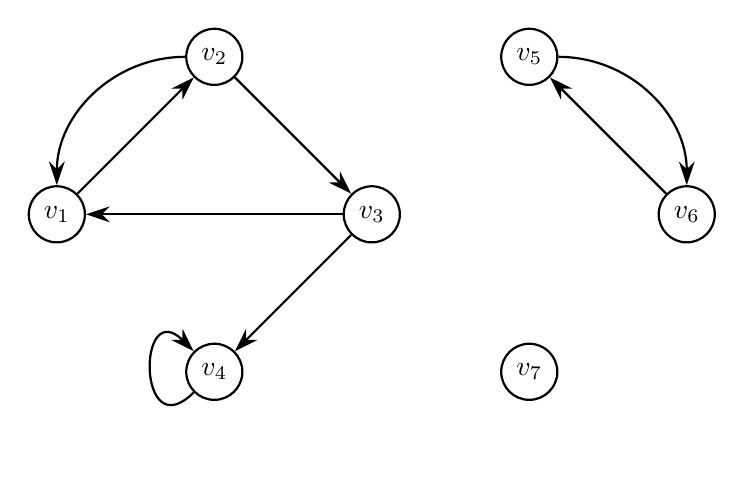
\begin{tikzpicture}
    % Define the nodes
    \node[mynode] (1) at (0, 0) {$v_1$};
    \node[mynode] (2) at (2, 2) {$v_2$};
    \node[mynode] (3) at (4, 0) {$v_3$};
    \node[mynode] (4) at (2, -2) {$v_4$};
    \node[mynode] (5) at (6, 2) {$v_5$};
    \node[mynode] (6) at (8, 0) {$v_6$};
    \node[mynode] (7) at (6, -2) {$v_7$};

    % Draw the edges
    \draw[myarrow] (1) -- (2);
    \draw[myarrow] (2) to[out=180, in=90] (1);
    \draw[myarrow] (4) to[out=225, in=135, looseness=5] (4); % This edge is a self-loop, corrected below
    \draw[myarrow] (2) -- (3);
    \draw[myarrow] (3) -- (4);
    \draw[myarrow] (3) -- (1);
    \draw[myarrow] (5) to[out=0, in=90] (6);
    \draw[myarrow] (6) -- (5);
\end{tikzpicture}
    \vspace{-10pt}
    \caption{Esempio di grafo orientato}
    \label{fig:directed-graph-example}
\end{figure}

Le cardintalit\`a degli insiemi di nodi e archi di un grafo orientato sono rispettivamente $|V| = n$ e $|E| = m$,
e vengono dette rispettivamente \textbf{ordine} e \textbf{dimensione} del grafo.

Essendo definiti su un insieme di elementi e di archi, possono essere definite relazioni di inclusione tra grafi.
Un grafo $G' = (V', E')$ \`e un sottografo di $G = (V, E)$, e lo si indica con $G' \subseteq G$ se $V' \subseteq V$
e $E' \subseteq E$. \newline
Inoltre, dato un certo insieme $V' \subseteq V$, si definisce il sottografo di $G$ \textbf{indotto} da $V'$, e lo si
indica con la notazione $G[V']$, il grafo avente come insieme di nodi $V'$ e come insieme di archi l'insieme di tutti
gli archi in $G$ che rappresentino relazioni tra tali nodi, ovvero il grafo $G' = (V', E')$ dove
$E' = \{ (u, v) \in E : u, v \in V'\}$. \newline

Essendo il contenuto informativo rilevante di un grafo orientato contenuto nei suoi archi, e quindi nelle relazioni
tra nodi, il concetto di eguaglianza tra grafi orientati non \`e banale.
Una relazione tra grafi orientati, utile per valutare la loro equivalenza in termini di informazione espressa,
\`e l'isomorfismo (dal greco \textit{iso} = uguale e \textit{morph\`e} = forma).
Così come per tutte le strutture matematiche, intuitivamente, due grafi si dicono \textbf{isomorfi} quando per ogni
parte della struttura di uno esiste una corrispondente parte della struttura dell'altro, e viceversa.
Formalmente, due grafi orientati $G = (V, E)$ e $H = (W, F)$ si dicono isomorfi, e lo si indica con $G \cong H$ se
esiste una biiezione $f: V \rightarrow W$ tale per cui $(u, v) \in E$ se e solo se $(f(u), f(v)) \in F$ per ogni
$u, v \in V$. \newline

\nlparagraph{Archi e nodi}\label{par:archi-e-nodi-di-un-grafo-orientato}

A seguire alcune definizioni relative ai nodi e agli archi di un grafo orientato: \newline

Sia $(u, v) \in E$ un arco di un grafo orientato $G = (V, E)$, allora:
\begin{itemize}
    \item l'arco $(u, v)$ \textbf{esce} dal nodo $u$ ed {entra} nel nodo $v$.
        Ad esempio, gli archi uscenti dal nodo $v_2$ nel grafo della figura~\ref{fig:directed-graph-example}
        sono $(v_2, v_1)$ e $(v_2, v_3)$, mentre l'unico arco entrante nel nodo $v_5$ \`e $(v_6, v_5)$.
    \item l'arco $(u, v)$ si dice \textbf{incidente} in entrambi i vertici $u$ e $v$.
    \item il nodo $v$ \`e detto \textbf{adiacente} al nodo $u$, in quanto esiste un arco $(u, v) \in E$.
\end{itemize}

Sia $v \in V$ un nodo di un grafo orientato $G = (V, E)$, allora:
\begin{itemize}
    \item il \textbf{grado uscente} di un nodo $v$ \`e il numero di archi che escono da $v$.
    \item il \textbf{grado entrante} di un nodo $v$ \`e il numero di archi che entrano in $v$.
    \item il \textbf{grado} di un nodo $v$ \`e la somma del grado uscente e del grado entrante di $v$.
\end{itemize}

\subsection{Cammini e Connessione tra nodi}\label{subsec:cammini}

\nlparagraph{Cammini}

I cammini sono concetti fondamentali della teoria dei grafi e sono alla base di molti algoritmi e problemi noti. \newline

Sia $G = (V, E)$ un grafo orientato, siano $u, v \in V$ due nodi di $G$, allora un \textbf{cammino} da $u$ a $v$ in $G$
\`e una sequenza ordinata di nodi $\langle v_0, v_1, \ldots, v_k \rangle$ tale che $(v_i, v_{i+1}) \in E$ per ogni
$i = 0, 1, \ldots, k-1$ con $v_1 = u$ e $v_k = v$.
La \textbf{lunghezza} k di un cammino \`e data dal numero di archi che lo compongono.
Ad esempio, $\langle v_1, v_2, v_3, v_4 \rangle$ \`e un cammino di lunghezza 3 nel grafo della
figura~\ref{fig:directed-graph-example}. \newline
Nel caso di grafi pesati, quindi aventi archi con un valore associato che ne indichi un costo, si definisce
\textbf{costo} di un cammino la somma dei pesi degli archi che lo compongono.
Inoltre, un \textbf{cammino minimo} tra una coppia di nodi $u$ e $v$ è un cammino di costo (o lunghezza, nel caso
di grafi non pesati) minore o uguale a quello di ogni altro cammino tra gli stessi nodi.

Se esiste un qualsiasi cammino $p$ da $u$ a $v$ in $G$, allora si dice che il nodo $v$ \`e \textbf{raggiungibile} da
$u$ attraverso $p$ in $G$, e questo pu\`o essere indicato con la notazione $u \overset{p}{\rightsquigarrow} v$. \newline

A seguire alcune definizioni relative ai cammini su un grafo orientato:

\begin{itemize}
    \item Un cammino si dice \textbf{semplice} se non contiene nodi ripetuti, ad eventuale eccezione del primo e
    dell'ultimo nodo.
    \item Un cammino si dice \textbf{elementare} se non contiene archi ripetuti. Si noti che un cammino semplice \`e
    sempre elementare.
    \item Un cammino $\langle v_0, v_1, \ldots, v_k \rangle$ di lunghezza $k \geq 1$ si dice \textbf{ciclo} se $v_1 = v_k$, ovvero se il
    suo nodo iniziale coincide con il suo nodo finale.
    Un \textbf{ciclo semplice} \`e un cammino in cui tutti i nodi sono distinti, ad eccezione del primo e dell'ultimo
    nodo, mentre un \textbf{ciclo elementare} (o \textbf{circuito}) \`e un ciclo in cui tutti gli archi sono distinti.
    Ad esempio, nel grafo in figura~\ref{fig:directed-graph-example}, il cammino $\langle v_1, v_2, v_3, v_1 \rangle$
    \`e un circuito semplice di lunghezza 3.
    Inoltre, un grafo diretto che non contiene cicli semplici \`e detto grafo diretto \textbf{aciciclico} (o
    \textbf{DAG}).
    \item Un cammino si dice \textbf{cammino hemiltoniano} in nel grafo $G$ se attraversa ogni nodo di $G$ esattamente
    una volta.
    \item Un cammino $\langle v_0, v_1, \ldots, v_k \rangle$ si dice \textbf{ciclo hemiltoniano} in nel grafo $G$ se
    esso \`e un ciclo e ogni nodo di $G$ appare una ed una sola volta tra i nodi $\langle v_0, v_1, \ldots,
    v_{k-1}\rangle$ e $v_k = v_0$.
    \item Un cammino si dice \textbf{cammino euleriano} nel grafo $G$ se attraversa ogni arco di $G$ esattamente una
    volta.
    \item Un cammino si dice \textbf{ciclo euleriano} nel grafo $G$ se esso \`e un ciclo e ogni arco di $G$ appare una
    ed una sola volta tra gli archi del ciclo.
\end{itemize}

\nlparagraph{Connessione tra nodi}

Una caratteristica importante dei grafi orientati, basata sul concetto di raggiungibilit\`a e adiacienza, e quindi
sui cammini, \`e la connessione dei suoi nodi.
\newline

Un grafo orientato $G = (V, E)$ si dice \textbf{fortemente connesso} se per ogni coppia di nodi $u, v \in V$ esiste un
cammino da $u$ a $v$. \newline
In un tale grafo, quindi, ogni nodo \`e mutualmente raggiungibile da ogni altro nodo.
Le \textbf{componenti fortemente connesse} di un grafo sono le classi di equivalenza dei nodi secondo la relazione
\"essere mutualmente raggiungibili\".
Ad esempio, nel grafo in figura~\ref{fig:directed-graph-example}, le componenti fortemente connesse sono
$\{\{v_1, v_2, v_3\}, \{v_4\}, \{v_5, v_6\}, \{v_7\}\}$.
Si noti che l'insieme di nodi $V$ di un grafo fortemente connesso \`e per definizione una unica componente connessa.
\newline

Un maggiore grado di connessione tra nodi \`e dato dalla presenza di singoli archi tra ogni coppia di nodi anzich\`e
di cammini. \newline
Un grafo orientato $G = (V, E)$ si dice \textbf{completo} se esiste un arco $(u, v) \in E$ per ogni coppia di nodi
distinti $u, v \in V$.
In un tale grafo, quindi, ogni coppia di nodi distinti \`e adiaciente.
Le \textbf{cricche} di un grafo sono le classi di equivalenza dei nodi secondo la relazione
\("\)essere mutualmente adiacienti\("\).
Ad esempio, nel grafo in figura~\ref{fig:directed-graph-example}, le cricche sono
$\{\{v_1, v_2\}, \{v_3\}, \{v_4\}, \{v_5, v_6\}, \{v_7\}\}$.
Si noti che l'insieme di nodi $V$ di un grafo completo \`e per definizione un'unica cricca.

\`E altresì possibile definire il concetto di \textbf{connettività} al livello globale di un grafo: informalmente,
un grafo ha una tanto più elevata connettività quanti più sono gli archi che devono essere rimossi per disconnettere
il grafo in più sottografi isolati.

\nlparagraph{Grafo trasposto}

Dato un grafo diretto $G = (V, E)$, il suo grafo trasposto $G^T = (V, E^T)$ \`e il grafo ottenuto invertendo
l'orientamento di tutti gli archi di $G$, ovvero $E^T = \{(u, v) \mid (v, u) \in E\}$.
 \'E interessante notare che $G^T$ ha le stesse componenti fortemente connesse di $G$: se un cammino da $u$ a $v$
esiste in $G$, allora esiste anche un cammino da $v$ a $u$ in $G^T$.
Essendo le componenti fortemente connesse basate sulla mutua raggiungibilit\`a dei nodi, esse non cambiano
quando si invertono gli archi.

Una procedura algoritmica per il calcolo di $G^T$ non farebbe altro che scorrere l'insieme di archi di $G$ e
invertirli, e sarebbe quindi di complessit\`a lineare.

\nlparagraph{Ordinamento topologico}

Dato un grafo diretto aciclico $G = (V, E)$, un ordinamento topologico di $G$ \`e una particolare sequenza
dei suoi nodi $\langle v_1, v_2, \ldots, v_n \rangle$ tale che per ogni arco $(v_i, v_j) \in E$, $i < j$.
Si noti, quindi, che un ordinamento topologico di un grafo diretto pu\`o esistere solo se il grafo non contiene
cicli.
Un ordinamento topologico fornisce una disposizione tale che i nodi raggiungibili da un certo nodo $v_i$ vengano
disposti dopo di esso, e che i nodi che $v_j$ pu\`o raggiungere vengano disposti dopo di esso.

Una procedura algoritmica per il calcolo di un ordinamento topologico di $G$ pu\`o essere effettuata tramite una
visita in profondit\`a del grafo, raccogliendo in una lista concatenata i nodi in ordine decrescente di tempo
di fine visita, man mano che vengono visitati.
Per via del normale costo di una visita in profondit\`a, la complessit\`a di tale procedura \`e lineare al
numero di nodi e di archi del grafo

\subsection{Visita in profondit\`a}
La visita in profondit\`a di un grafo (in inglese \textit{depth-first search} o \textit{DFS}) \`e un particolare
algoritmo di visita che, in quanto tale, permette di visitare tutti i nodi di un grafo partendo da un nodo iniziale,
e di scoprire tutti i nodi raggiungibili da esso.
Ci\`o viene fatto in modo ricorsivo: nel corso della visita di un nodo si considerano uno ad uno i nodi ad esso
adiacenti, e ai nodi non ancora marcati come visitati viene applicata immediatamente la stessa procedura di visita.

\begin{algorithm}[H]
    \caption{DFS($G$)}\label{alg:dfs}
    \begin{algorithmic}[1]
        \For {$v \in G.V$}
            \State $v.color \coloneqq$ WHITE
            \State $u.\pi \coloneqq$ NIL
        \EndFor
        \State $time \coloneqq 0$
        \For{$v \in G.V$}
            \If {$v.color ==$ WHITE}
                \State $DFS-VISIT(G, v)$
            \EndIf
        \EndFor
    \end{algorithmic}
\end{algorithm}
\begin{algorithm}[H]
    \caption{DFS-VISIT($G$, $u$)}\label{alg:dfs-visit}
    \begin{algorithmic}[1]
        \State $u.color \coloneqq$ GRAY
        \State $time \coloneqq time + 1$
        \State $u.d \coloneqq time$
        \For {$v \in G.Adj[u]$}
            \If {$v.color ==$ WHITE}
                \State $v.\pi \coloneqq u$
                \State $DFS-VISIT(G, v)$
            \EndIf
        \EndFor
        \State $u.color \coloneqq$ BLACK
        \State $time \coloneqq time + 1$
        \State $u.f \coloneqq time$
    \end{algorithmic}
\end{algorithm}


\begin{figure}
    \resizebox{!}{3.07cm}{
    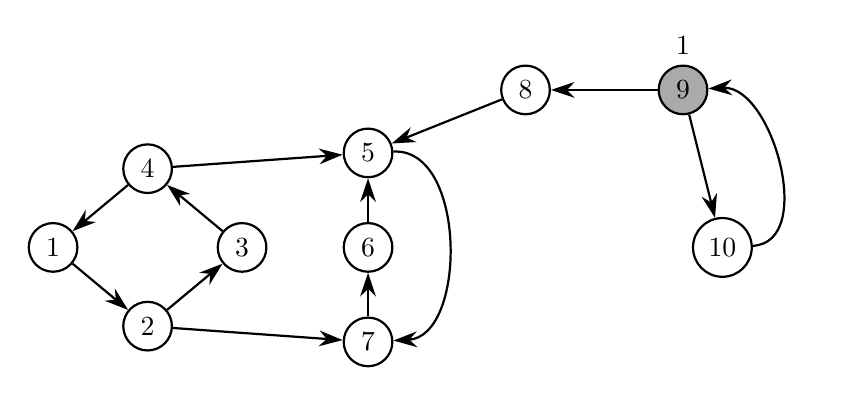
\begin{tikzpicture}
        %comp 1
        \node[mynode](n1) at (0,0){1};
        \node[mynode](n2) at (1.2,-1){2};
        \node[mynode](n3) at (1.2, 1){4};
        \node[mynode](n4) at (2.4, 0){3};
        \draw[myarrow](n1)--(n2);
        \draw[myarrow](n3)--(n1);
        \draw[myarrow](n4)--(n3);
        \draw[myarrow](n2)--(n4);
        %comp 2
        \node[mynode](n5) at (4,1.2){5};
        \node[mynode](n6) at (4,0){6};
        \node[mynode](n7) at (4, -1.2){7};
        \draw[myarrow](n6) -- (n5);
        \draw[myarrow](n5) to[out=3,in=3] (n7);
        \draw[myarrow](n7) -- (n6);

        %comp edges
        \draw[myarrow](n3) -- (n5);
        \draw[myarrow](n2) -- (n7);
        %comp 3
        \node[mynode](n8) at (6, 2){8};
        %comp 4
        \node[mynode, label=above:{$1$}, fill={rgb:black,1;white,2}](n9) at (8, 2){9};
        \node[mynode](na) at (8.5, 0){10};
        \draw[myarrow](n9) -- (n8);
        \draw[myarrow](na) to[out=3,in=3] (n9);
        \draw[myarrow](n9) -- (na);
        \draw[myarrow](n8) -- (n5);
    \end{tikzpicture} \quad \quad
    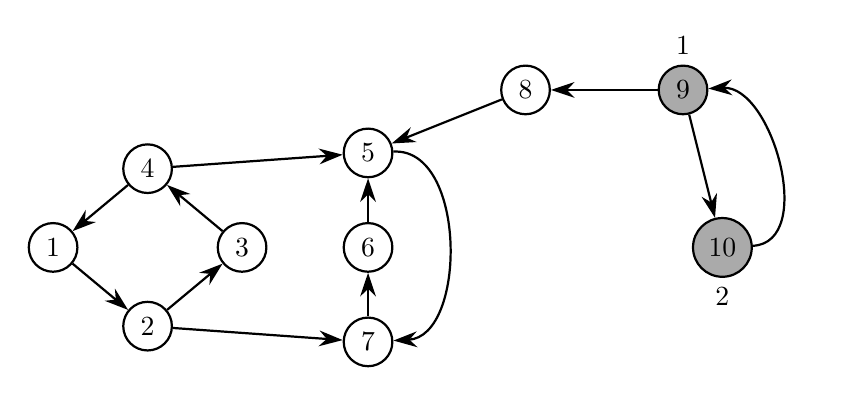
\begin{tikzpicture}
        %comp 1
        % \node[mynode, fill=black](n1) at (0,0){\textcolor{white}{1}};
        \node[mynode](n1) at (0,0){1};
        \node[mynode](n2) at (1.2,-1){2};
        \node[mynode](n3) at (1.2, 1){4};
        \node[mynode](n4) at (2.4, 0){3};
        \draw[myarrow](n1)--(n2);
        \draw[myarrow](n3)--(n1);
        \draw[myarrow](n4)--(n3);
        \draw[myarrow](n2)--(n4);
        %comp 2
        \node[mynode](n5) at (4,1.2){5};
        \node[mynode](n6) at (4,0){6};
        \node[mynode](n7) at (4, -1.2){7};
        \draw[myarrow](n6) -- (n5);
        \draw[myarrow](n5) to[out=3,in=3] (n7);
        \draw[myarrow](n7) -- (n6);

        %comp edges
        \draw[myarrow](n3) -- (n5);
        \draw[myarrow](n2) -- (n7);
        %comp 3
        \node[mynode](n8) at (6, 2){8};
        %comp 4
        \node[mynode, label=above:{$1$}, fill={rgb:black,1;white,2}](n9) at (8, 2){9};
        \node[mynode, label=below:{$2$}, fill={rgb:black,1;white,2}](na) at (8.5, 0){10};
        \draw[myarrow](n9) -- (n8);
        \draw[myarrow](na) to[out=3,in=3] (n9);
        \draw[myarrow](n9) -- (na);
        \draw[myarrow](n8) -- (n5);
    \end{tikzpicture}
}
\resizebox{!}{3.07cm}{
    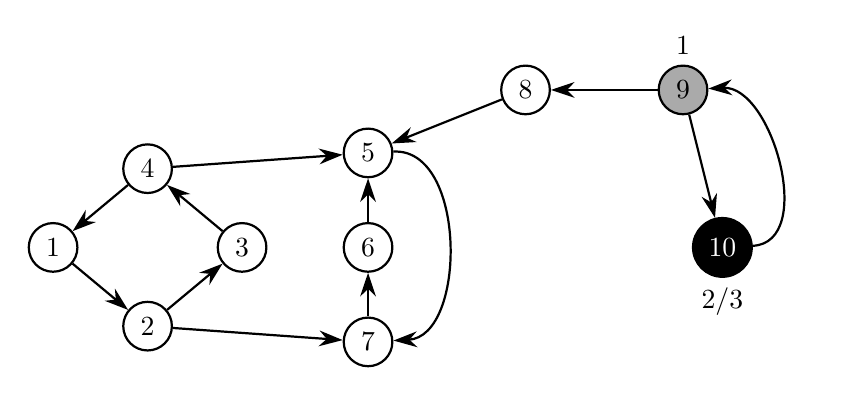
\begin{tikzpicture}
        %comp 1
        \node[mynode](n1) at (0,0){1};
        \node[mynode](n2) at (1.2,-1){2};
        \node[mynode](n3) at (1.2, 1){4};
        \node[mynode](n4) at (2.4, 0){3};
        \draw[myarrow](n1)--(n2);
        \draw[myarrow](n3)--(n1);
        \draw[myarrow](n4)--(n3);
        \draw[myarrow](n2)--(n4);
        %comp 2
        \node[mynode](n5) at (4,1.2){5};
        \node[mynode](n6) at (4,0){6};
        \node[mynode](n7) at (4, -1.2){7};
        \draw[myarrow](n6) -- (n5);
        \draw[myarrow](n5) to[out=3,in=3] (n7);
        \draw[myarrow](n7) -- (n6);

        %comp edges
        \draw[myarrow](n3) -- (n5);
        \draw[myarrow](n2) -- (n7);
        %comp 3
        \node[mynode](n8) at (6, 2){8};
        %comp 4
        \node[mynode, label=above:{$1$}, fill={rgb:black,1;white,2}](n9) at (8, 2){9};
        \node[mynode, label=below:{$2/3$}, fill=black](na) at (8.5, 0){\textcolor{white}{10}};
        \draw[myarrow](n9) -- (n8);
        \draw[myarrow](na) to[out=3,in=3] (n9);
        \draw[myarrow](n9) -- (na);
        \draw[myarrow](n8) -- (n5);
    \end{tikzpicture} \quad \quad
    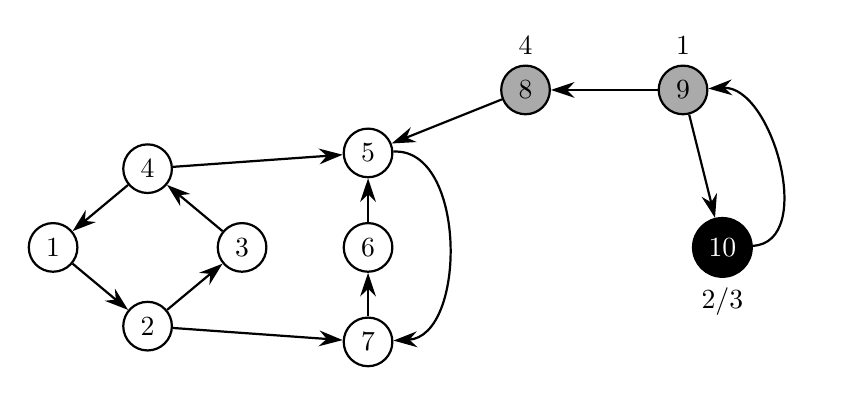
\begin{tikzpicture}
        %comp 1
        \node[mynode](n1) at (0,0){1};
        \node[mynode](n2) at (1.2,-1){2};
        \node[mynode](n3) at (1.2, 1){4};
        \node[mynode](n4) at (2.4, 0){3};
        \draw[myarrow](n1)--(n2);
        \draw[myarrow](n3)--(n1);
        \draw[myarrow](n4)--(n3);
        \draw[myarrow](n2)--(n4);
        %comp 2
        \node[mynode](n5) at (4,1.2){5};
        \node[mynode](n6) at (4,0){6};
        \node[mynode](n7) at (4, -1.2){7};
        \draw[myarrow](n6) -- (n5);
        \draw[myarrow](n5) to[out=3,in=3] (n7);
        \draw[myarrow](n7) -- (n6);

        %comp edges
        \draw[myarrow](n3) -- (n5);
        \draw[myarrow](n2) -- (n7);
        %comp 3
        \node[mynode, label=above:{$4$}, fill={rgb:black,1;white,2}](n8) at (6, 2){8};
        %comp 4
        \node[mynode, label=above:{$1$}, fill={rgb:black,1;white,2}](n9) at (8, 2){9};
        \node[mynode, label=below:{$2/3$}, fill=black](na) at (8.5, 0){\textcolor{white}{10}};
        \draw[myarrow](n9) -- (n8);
        \draw[myarrow](na) to[out=3,in=3] (n9);
        \draw[myarrow](n9) -- (na);
        \draw[myarrow](n8) -- (n5);
    \end{tikzpicture}
}
\resizebox{!}{3.416cm}{
    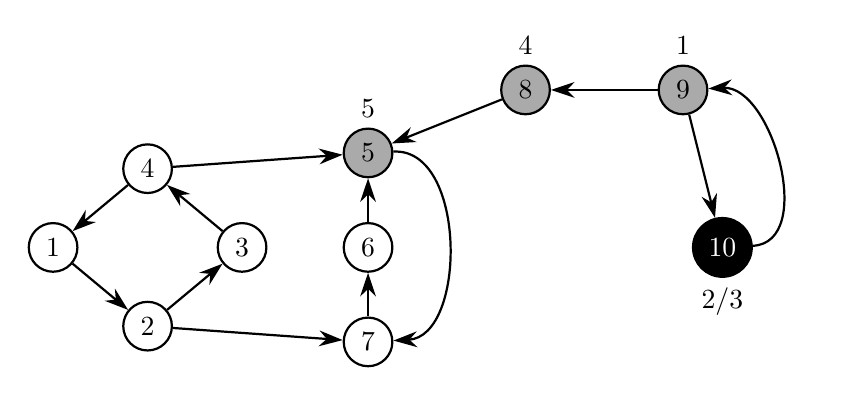
\begin{tikzpicture}
        %comp 1

        \node[mynode](n1) at (0,0){1};
        \node[mynode](n2) at (1.2,-1){2};
        \node[mynode](n3) at (1.2, 1){4};
        \node[mynode](n4) at (2.4, 0){3};
        \draw[myarrow](n1)--(n2);
        \draw[myarrow](n3)--(n1);
        \draw[myarrow](n4)--(n3);
        \draw[myarrow](n2)--(n4);
        %comp 2
        \node[mynode, label=above:{$5$}, fill={rgb:black,1;white,2}](n5) at (4,1.2){5};
        \node[mynode](n6) at (4,0){6};
        \node[mynode](n7) at (4, -1.2){7};
        \draw[myarrow](n6) -- (n5);
        \draw[myarrow](n5) to[out=3,in=3] (n7);
        \draw[myarrow](n7) -- (n6);

        %comp edges
        \draw[myarrow](n3) -- (n5);
        \draw[myarrow](n2) -- (n7);
        %comp 3
        \node[mynode, label=above:{$4$}, fill={rgb:black,1;white,2}](n8) at (6, 2){8};
        %comp 4
        \node[mynode, label=above:{$1$}, fill={rgb:black,1;white,2}](n9) at (8, 2){9};
        \node[mynode, label=below:{$2/3$}, fill=black](na) at (8.5, 0){\textcolor{white}{10}};
        \draw[myarrow](n9) -- (n8);
        \draw[myarrow](na) to[out=3,in=3] (n9);
        \draw[myarrow](n9) -- (na);
        \draw[myarrow](n8) -- (n5);
    \end{tikzpicture} \quad \quad
    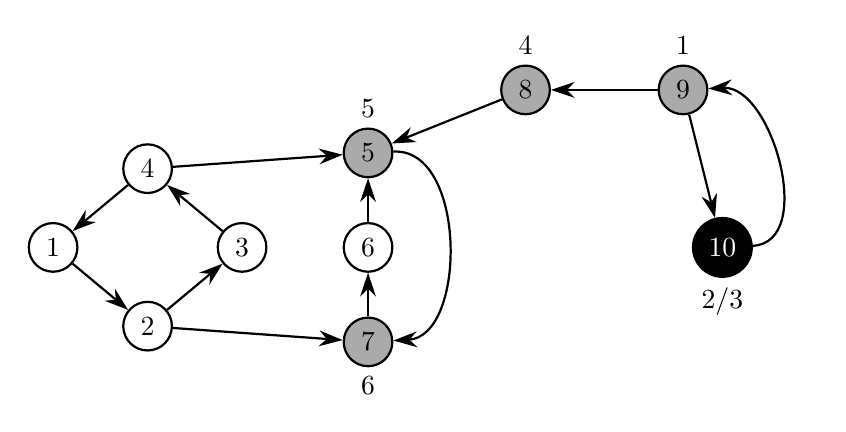
\begin{tikzpicture}
        %comp 1

        \node[mynode](n1) at (0,0){1};
        \node[mynode](n2) at (1.2,-1){2};
        \node[mynode](n3) at (1.2, 1){4};
        \node[mynode](n4) at (2.4, 0){3};
        \draw[myarrow](n1)--(n2);
        \draw[myarrow](n3)--(n1);
        \draw[myarrow](n4)--(n3);
        \draw[myarrow](n2)--(n4);
        %comp 2
        \node[mynode, label=above:{$5$}, fill={rgb:black,1;white,2}](n5) at (4,1.2){5};
        \node[mynode](n6) at (4,0){6};
        \node[mynode, label=below:{$6$}, fill={rgb:black,1;white,2}](n7) at (4, -1.2){7};
        \draw[myarrow](n6) -- (n5);
        \draw[myarrow](n5) to[out=3,in=3] (n7);
        \draw[myarrow](n7) -- (n6);

        %comp edges
        \draw[myarrow](n3) -- (n5);
        \draw[myarrow](n2) -- (n7);
        %comp 3
        \node[mynode, label=above:{$4$}, fill={rgb:black,1;white,2}](n8) at (6, 2){8};
        %comp 4
        \node[mynode, label=above:{$1$}, fill={rgb:black,1;white,2}](n9) at (8, 2){9};
        \node[mynode, label=below:{$2/3$}, fill=black](na) at (8.5, 0){\textcolor{white}{10}};
        \draw[myarrow](n9) -- (n8);
        \draw[myarrow](na) to[out=3,in=3] (n9);
        \draw[myarrow](n9) -- (na);
        \draw[myarrow](n8) -- (n5);
    \end{tikzpicture}
}
\resizebox{!}{3.416cm}{
    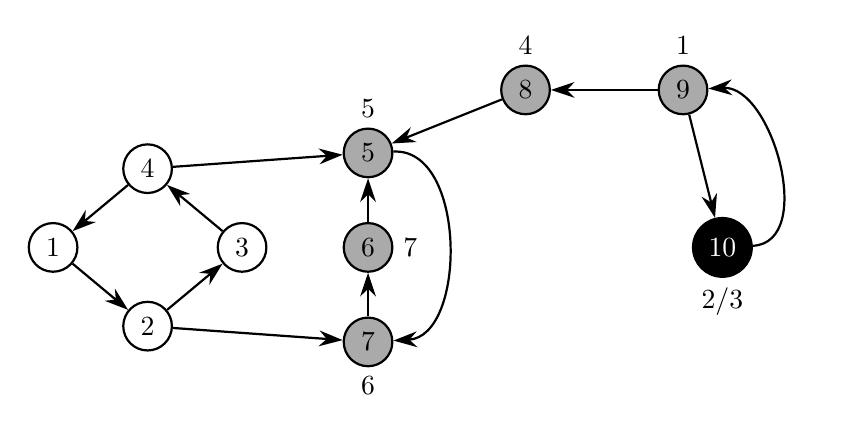
\begin{tikzpicture}
        %comp 1
        \node[mynode](n1) at (0,0){1};
        \node[mynode](n2) at (1.2,-1){2};
        \node[mynode](n3) at (1.2, 1){4};
        \node[mynode](n4) at (2.4, 0){3};
        \draw[myarrow](n1)--(n2);
        \draw[myarrow](n3)--(n1);
        \draw[myarrow](n4)--(n3);
        \draw[myarrow](n2)--(n4);
        %comp 2
        \node[mynode, label=above:{$5$}, fill={rgb:black,1;white,2}](n5) at (4,1.2){5};
        \node[mynode, label=right:{$7$}, fill={rgb:black,1;white,2}](n6) at (4,0){6};
        \node[mynode, label=below:{$6$}, fill={rgb:black,1;white,2}](n7) at (4, -1.2){7};
        \draw[myarrow](n6) -- (n5);
        \draw[myarrow](n5) to[out=3,in=3] (n7);
        \draw[myarrow](n7) -- (n6);

        %comp edges
        \draw[myarrow](n3) -- (n5);
        \draw[myarrow](n2) -- (n7);
        %comp 3
        \node[mynode, label=above:{$4$}, fill={rgb:black,1;white,2}](n8) at (6, 2){8};
        %comp 4
        \node[mynode, label=above:{$1$}, fill={rgb:black,1;white,2}](n9) at (8, 2){9};
        \node[mynode, label=below:{$2/3$}, fill=black](na) at (8.5, 0){\textcolor{white}{10}};
        \draw[myarrow](n9) -- (n8);
        \draw[myarrow](na) to[out=3,in=3] (n9);
        \draw[myarrow](n9) -- (na);
        \draw[myarrow](n8) -- (n5);
    \end{tikzpicture} \quad \quad
    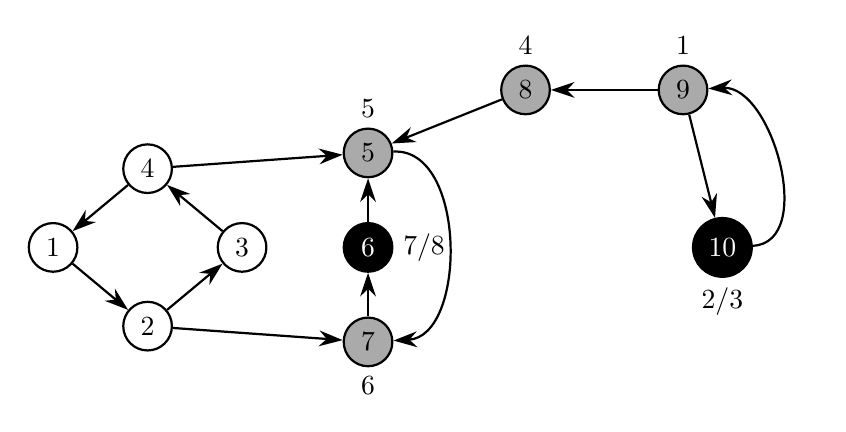
\begin{tikzpicture}
        %comp 1
        \node[mynode](n1) at (0,0){1};
        \node[mynode](n2) at (1.2,-1){2};
        \node[mynode](n3) at (1.2, 1){4};
        \node[mynode](n4) at (2.4, 0){3};
        \draw[myarrow](n1)--(n2);
        \draw[myarrow](n3)--(n1);
        \draw[myarrow](n4)--(n3);
        \draw[myarrow](n2)--(n4);
        %comp 2
        \node[mynode, label=above:{$5$}, fill={rgb:black,1;white,2}](n5) at (4,1.2){5};
        \node[mynode, label=right:{$7/8$}, fill=black](n6) at (4,0){\textcolor{white}{6}};
        \node[mynode, label=below:{$6$}, fill={rgb:black,1;white,2}](n7) at (4, -1.2){7};
        \draw[myarrow](n6) -- (n5);
        \draw[myarrow](n5) to[out=3,in=3] (n7);
        \draw[myarrow](n7) -- (n6);

        %comp edges
        \draw[myarrow](n3) -- (n5);
        \draw[myarrow](n2) -- (n7);
        %comp 3
        \node[mynode, label=above:{$4$}, fill={rgb:black,1;white,2}](n8) at (6, 2){8};
        %comp 4
        \node[mynode, label=above:{$1$}, fill={rgb:black,1;white,2}](n9) at (8, 2){9};
        \node[mynode, label=below:{$2/3$}, fill=black](na) at (8.5, 0){\textcolor{white}{10}};
        \draw[myarrow](n9) -- (n8);
        \draw[myarrow](na) to[out=3,in=3] (n9);
        \draw[myarrow](n9) -- (na);
        \draw[myarrow](n8) -- (n5);
    \end{tikzpicture}
}
\resizebox{!}{3.5cm}{
    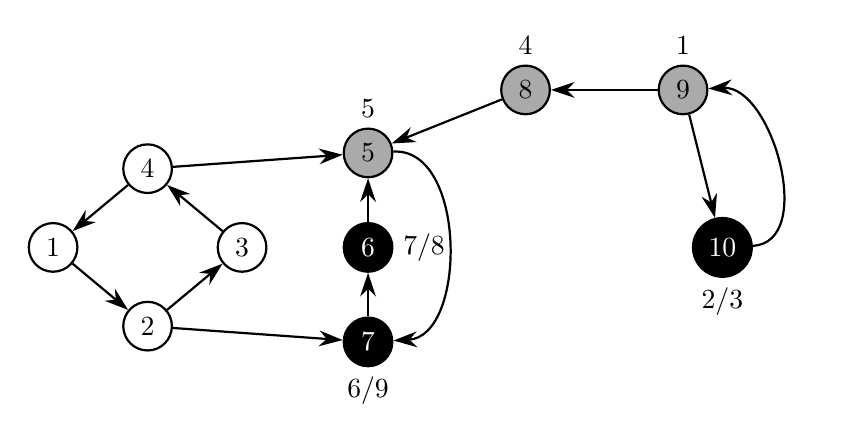
\begin{tikzpicture}
        %comp 1
        \node[mynode](n1) at (0,0){1};
        \node[mynode](n2) at (1.2,-1){2};
        \node[mynode](n3) at (1.2, 1){4};
        \node[mynode](n4) at (2.4, 0){3};
        \draw[myarrow](n1)--(n2);
        \draw[myarrow](n3)--(n1);
        \draw[myarrow](n4)--(n3);
        \draw[myarrow](n2)--(n4);
        %comp 2
        \node[mynode, label=above:{$5$}, fill={rgb:black,1;white,2}](n5) at (4,1.2){5};
        \node[mynode, label=right:{$7/8$}, fill=black](n6) at (4,0){\textcolor{white}{6}};
        \node[mynode, label=below:{$6/9$}, fill=black](n7) at (4, -1.2){\textcolor{white}{7}};
        \draw[myarrow](n6) -- (n5);
        \draw[myarrow](n5) to[out=3,in=3] (n7);
        \draw[myarrow](n7) -- (n6);

        %comp edges
        \draw[myarrow](n3) -- (n5);
        \draw[myarrow](n2) -- (n7);
        %comp 3
        \node[mynode, label=above:{$4$}, fill={rgb:black,1;white,2}](n8) at (6, 2){8};
        %comp 4
        \node[mynode, label=above:{$1$}, fill={rgb:black,1;white,2}](n9) at (8, 2){9};
        \node[mynode, label=below:{$2/3$}, fill=black](na) at (8.5, 0){\textcolor{white}{10}};
        \draw[myarrow](n9) -- (n8);
        \draw[myarrow](na) to[out=3,in=3] (n9);
        \draw[myarrow](n9) -- (na);
        \draw[myarrow](n8) -- (n5);
    \end{tikzpicture} \quad \quad
    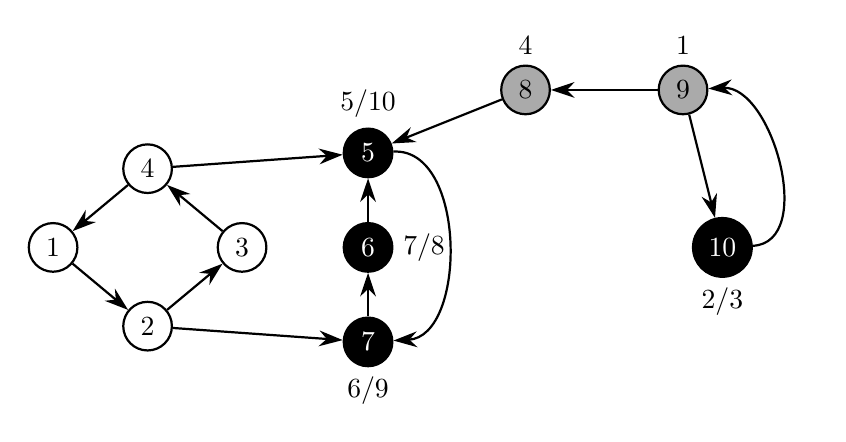
\begin{tikzpicture}
        % comp 1
        \node[mynode](n1) at (0,0){1};
        \node[mynode](n2) at (1.2,-1){2};
        \node[mynode](n3) at (1.2, 1){4};
        \node[mynode](n4) at (2.4, 0){3};
        \draw[myarrow](n1)--(n2);
        \draw[myarrow](n3)--(n1);
        \draw[myarrow](n4)--(n3);
        \draw[myarrow](n2)--(n4);
        %comp 2
        \node[mynode, label=above:{$5/10$}, fill=black](n5) at (4,1.2){\textcolor{white}{5}};
        \node[mynode, label=right:{$7/8$}, fill=black](n6) at (4,0){\textcolor{white}{6}};
        \node[mynode, label=below:{$6/9$}, fill=black](n7) at (4, -1.2){\textcolor{white}{7}};
        \draw[myarrow](n6) -- (n5);
        \draw[myarrow](n5) to[out=3,in=3] (n7);
        \draw[myarrow](n7) -- (n6);

        %comp edges
        \draw[myarrow](n3) -- (n5);
        \draw[myarrow](n2) -- (n7);
        %comp 3
        \node[mynode, label=above:{$4$}, fill={rgb:black,1;white,2}](n8) at (6, 2){8};
        %comp 4
        \node[mynode, label=above:{$1$}, fill={rgb:black,1;white,2}](n9) at (8, 2){9};
        \node[draw, thick, circle, label=below:{$2/3$}, fill=black](na) at (8.5, 0){\textcolor{white}{10}};
        \draw[myarrow](n9) -- (n8);
        \draw[myarrow](na) to[out=3,in=3] (n9);
        \draw[myarrow](n9) -- (na);
        \draw[myarrow](n8) -- (n5);
    \end{tikzpicture}
}
\resizebox{!}{3.59cm}{
    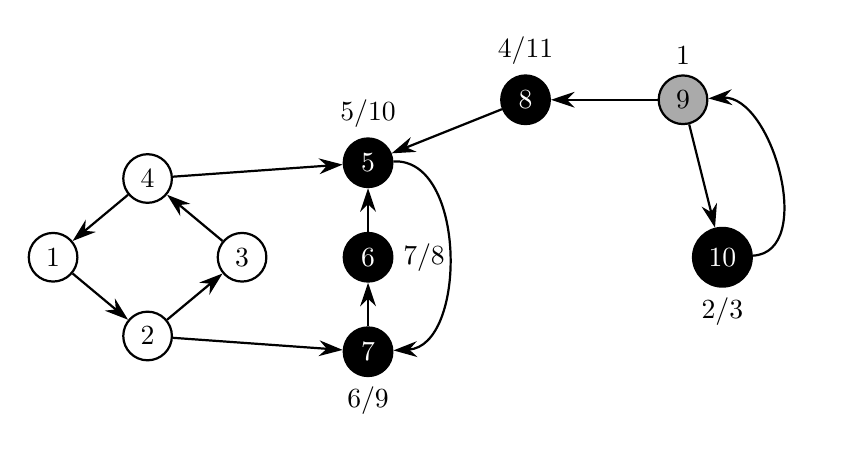
\begin{tikzpicture}
        %comp 1
        % \node[mynode, fill=black](n1) at (0,0){\textcolor{white}{1}};
        \node[mynode](n1) at (0,0){1};
        \node[mynode](n2) at (1.2,-1){2};
        \node[mynode](n3) at (1.2, 1){4};
        \node[mynode](n4) at (2.4, 0){3};
        \draw[myarrow](n1)--(n2);
        \draw[myarrow](n3)--(n1);
        \draw[myarrow](n4)--(n3);
        \draw[myarrow](n2)--(n4);
        %comp 2
        \node[mynode, label=above:{$5/10$}, fill=black](n5) at (4,1.2){\textcolor{white}{5}};
        \node[mynode, label=right:{$7/8$}, fill=black](n6) at (4,0){\textcolor{white}{6}};
        \node[mynode, label=below:{$6/9$}, fill=black](n7) at (4, -1.2){\textcolor{white}{7}};
        \draw[myarrow](n6) -- (n5);
        \draw[myarrow](n5) to[out=3,in=3] (n7);
        \draw[myarrow](n7) -- (n6);

        %comp edges
        \draw[myarrow](n3) -- (n5);
        \draw[myarrow](n2) -- (n7);
        %comp 3
        \node[mynode, label=above:{$4/11$}, fill=black](n8) at (6, 2){\textcolor{white}{8}};
        %comp 4
        \node[mynode, label=above:{$1$}, fill={rgb:black,1;white,2}](n9) at (8, 2){9};
        \node[mynode, label=below:{$2/3$}, fill=black](na) at (8.5, 0){\textcolor{white}{10}};
        \draw[myarrow](n9) -- (n8);
        \draw[myarrow](na) to[out=3,in=3] (n9);
        \draw[myarrow](n9) -- (na);
        \draw[myarrow](n8) -- (n5);
    \end{tikzpicture} \quad \quad
    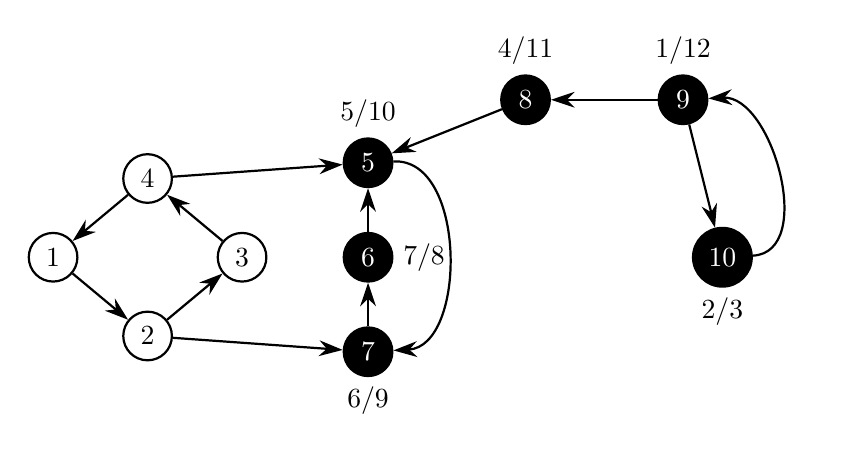
\begin{tikzpicture}
        %comp 1
        % \node[mynode, fill=black](n1) at (0,0){\textcolor{white}{1}};
        \node[mynode](n1) at (0,0){1};
        \node[mynode](n2) at (1.2,-1){2};
        \node[mynode](n3) at (1.2, 1){4};
        \node[mynode](n4) at (2.4, 0){3};
        \draw[myarrow](n1)--(n2);
        \draw[myarrow](n3)--(n1);
        \draw[myarrow](n4)--(n3);
        \draw[myarrow](n2)--(n4);
        %comp 2
        \node[mynode, label=above:{$5/10$}, fill=black](n5) at (4,1.2){\textcolor{white}{5}};
        \node[mynode, label=right:{$7/8$}, fill=black](n6) at (4,0){\textcolor{white}{6}};
        \node[mynode, label=below:{$6/9$}, fill=black](n7) at (4, -1.2){\textcolor{white}{7}};
        \draw[myarrow](n6) -- (n5);
        \draw[myarrow](n5) to[out=3,in=3] (n7);
        \draw[myarrow](n7) -- (n6);

        %comp edges
        \draw[myarrow](n3) -- (n5);
        \draw[myarrow](n2) -- (n7);
        %comp 3
        \node[mynode, label=above:{$4/11$}, fill=black](n8) at (6, 2){\textcolor{white}{8}};
        %comp 4
        \node[mynode, label=above:{$1/12$}, fill=black](n9) at (8, 2){\textcolor{white}{9}};
        \node[mynode, label=below:{$2/3$}, fill=black](na) at (8.5, 0){\textcolor{white}{10}};
        \draw[myarrow](n9) -- (n8);
        \draw[myarrow](na) to[out=3,in=3] (n9);
        \draw[myarrow](n9) -- (na);
        \draw[myarrow](n8) -- (n5);
    \end{tikzpicture}
}

    \caption{Esempio di esecuzione di una visita in profondit\`a su un grafo diretto}
    \label{fig:dfs-example}
\end{figure}

Nel corso dell'algoritmo i nodi vengono colorati in tre colori: bianco, grigio e nero, ad indicare rispettivamente
che il nodo non \`e stato visitato, che \`e in fase di visita e che \`e stato visitato.
Questo permette di non incorrere in cicli di visita infiniti nel caso non si stia visitando un grafo aciclico.
Nel corso dell'algoritmo vengono anche assegnati ai nodi due valori interi: il tempo di scoperta $d$ e il tempo di
fine visita $f$, che permettono di determinare, rispettivamente, il momento in cui i nodi vengono scoperti e colorati
di grigio e il tempo in cui la visita di un nodo termina, colorandosi di nero.
Un attributo aggiuntivo, il predecessore $\pi$, permette di memorizzare il nodo da cui si \`e scoperto il nodo
corrente e, con esso, di ricostruire il cammino di visita sotto forma di albero, detto albero di visita in profondit\`a.
\newline

In figura~\ref{fig:dfs-example} \`e rappresentato un esempio di esecuzione della procedura DFS-VISIT su un grafo
diretto, eseguita a partire dal nodo con etichetta $9$, in cui lo stato del grafo \`e rappresentato ad ogni
incremento della variabile $time$. \newline

La procedura si mantiene in tempo lineare rispetto al numero di nodi e di archi del grafo, in quanto
ogni nodo viene visitato una sola volta e ogni arco viene esaminato al massimo una volta.
\section{Algoritmi di enumerazione}\label{sec:algoritmi-di-enumerazione}

In informatica, un \textit{algoritmo di enumerazione} \`e un algoritmo che elenca tutte le possibili risposte ad un
problema computazionale in modo sistematico e completo. Tali algoritmi sono quindi progettati per ricevere un
determinato input, generare una lista esaustiva di tutte le possibili soluzioni senza duplicati e, solo allora,
terminare.
Quando si parla di algoritmi di enumerazione applicati al dominio dei grafi, allora spesso si intende il processo di
identificazione di sottoinsiemi di nodi o archi che soddisfano determinate caratteristiche.
In questa sezione si tratteranno e analizzeranno alcuni utili algoritmi di enumerazione presenti in letteratura per
il riconoscimento di pattern strutturali all'interno di grafi.
In particolare, si discuteranno algoritmi per l'enumerazione di componenti fortemente connesse, di cricche e di
circuiti semplici.
Questi algoritmi costituiranno il \"motore\" degli algoritmi presentati nei capitoli successivi, e saranno di
importanza fondamentale alla definizione degli algoritmi di contrazione usati per la costruzione di grafi multi-livello.

\subsection{Enumerazione di componenti fortemente connesse}\label{subsec:enumerazione-di-componenti-fortemente-connesse}

Come precedentemente citato, una componente fortemente connessa di un grafo diretto \`e un sottoinsieme massimale
di nodi che siano mutualmente raggiungibili, ovvero tali che per ogni coppia di nodi $u$ e $v$ della componente esiste
un cammino da $u$ a $v$ e viceversa.
In questa sezione si discuter\`a un classico algoritmo di enumerazione delle componenti fortemente connesse, chiamato
da alcuni testi come l'algoritmo di Kosaraju~\cite{SHARIR198167}.

\nlparagraph{Algoritmo di Kosaraju}

L'algoritmo di Kosaraju (anche noto come algoritmo di Kosaraju-Sharir) è un algoritmo per l'enumerazione
delle componenti fortemente connesse di un grafo diretto dalla complessità lineare scoperto nel 1978 da S. Rao
Kosaraju, ma pubblicato solamente nel 1981 da Micha Sharir, che lo scoprì indipendentemente.
Esso sfrutta il principio per cui le componenti fortemente connesse di un grafo diretto sono le stesse del suo grafo
trasposto, ovvero il grafo ottenuto invertendo l'orientamento di tutti gli archi. \newline

\begin{algorithm}[H] \floatname{algorithm}{Algoritmo}
    \caption{KOSARAJU-ALGORITHM($G$)}\label{alg:cap2}
    \begin{algorithmic}[1]
        \State Esegui $DFS(G)$ per calcolare il tempo di fine visita $u.f$ per ogni nodo $u$ in $G$
        \State Calcola $G^T$
        \State Esegui $DFS(G^T)$, considerando $G.V$ in ordine decrescente di tempo di fine visita
        \State Fornisci in output ogni albero di visita in profondit\`a come componente fortemente connessa di $G$
    \end{algorithmic}
\end{algorithm}

Come descritto dallo pseudocodice, l'algoritmo di Kosaraju esegue due visite in profondit\`a, una sul grafo
originale $G$ e una sul grafo trasposto $G^T$, in cui la seconda visita viene effettuata secondo l'ordinamento
ottenuto dalla prima.
Le motivazioni per cui la procedura di visita a riga 3 permette di visitare una componente fortemente
connessa alla volta per ogni iterazione del ciclo for principale possono essere riassunte dai seguenti punti:
\begin{itemize}
    \item La condensazione di $G$ \`e un grafo aciclico, e quindi ammette un ordinamento topologico.
        Questo vuol dire che se esiste un cammino $u \rightsquigarrow v$ in $G$, con $u$ e $v$ nodi di componenti
        fortemente connesse distinte, allora di certo non pu\`o esistere un cammino $v \rightsquigarrow u$ in $G$,
        altrimenti i nodi in entrambe le componenti connesse sarebbero tutti mutualmente raggiungibili tra loro, e
        costituirebbero una unica componente fortemente connessa.
    \item Se $C$ e $C'$ sono componenti fortemente connesse di $G$ distinte ed esiste in $G$ un cammino
        $u \rightsquigarrow v$ con $u \in C$ e $v \in C'$, allora il tempo di fine visita massimo tra i nodi di $C$
        sar\`a maggiore del tempo di fine visita massimo tra i nodi di $C'$.
        Infatti, supponendo che venga visitato prima $u$, tutti i nodi raggiungibili da $u$, incluso $v$ e tutti i nodi
        in $C'$, saranno visitati prima che la visita di $u$ termini.
        Al contempo, supponendo che venga visitato prima $v$, allora nessun nodo di $C$ verr\`a visitato prima che
        la visita di $v$ termini, in quanto, come detto nel primo punto, l'esistenza di un cammino
        $u \rightsquigarrow v$ esculde l'esistenza di un cammino $v \rightsquigarrow u$.
    \item Considerare i nodi in ordine decrescente di tempo di fine visita permette di visitare prima le componenti
        fortemente connesse meno \"profonde\", ovvero quelle che non contengono nodi raggiungibili da altre
        componenti fortemente connesse.
        In altre parole, le componenti meno profonde sono le prime ad apparire nell'ordinamento topologico della
        condensazione.
    \item Invertendo il senso degli archi e visitando prima le componenti fortemente connesse meno profonde in $G$, si
        garantisce che non si possano raggiungere nodi di altre componenti, ma solo nodi della stessa componente.
        Invertendo il senso degli archi, infatti, si inverte l'ordinamento topologico della condensazione, visitando
        prima le compoenenti che si trovano in fondo al nuovo ordinamento.
\end{itemize}

\begin{figure}
    \resizebox{!}{4cm}{
        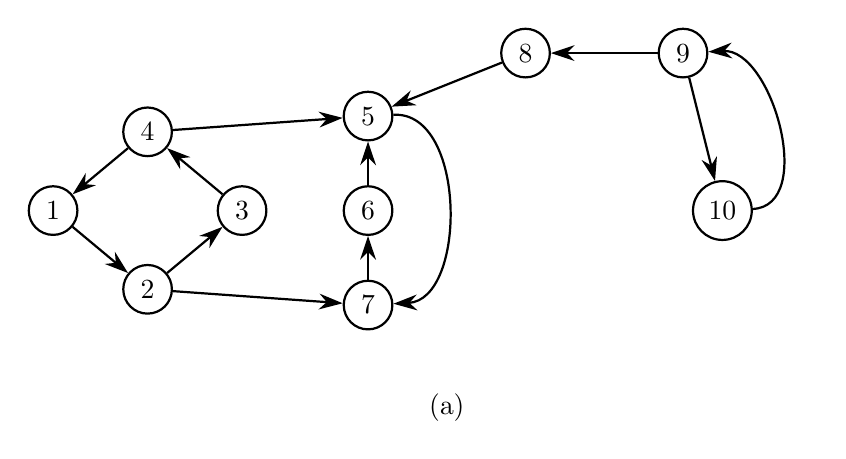
\begin{tikzpicture}
    %comp 1
    \node[mynode](n1) at (0,0){1};
    \node[mynode](n2) at (1.2,-1){2};
    \node[mynode](n3) at (1.2, 1){4};
    \node[mynode](n4) at (2.4, 0){3};
    \draw[myarrow](n1)--(n2);
    \draw[myarrow](n3)--(n1);
    \draw[myarrow](n4)--(n3);
    \draw[myarrow](n2)--(n4);
    %comp 2
    \node[mynode](n5) at (4,1.2){5};
    \node[mynode](n6) at (4,0){6};
    \node[mynode](n7) at (4, -1.2){7};
    \draw[myarrow](n6) -- (n5);
    \draw[myarrow](n5) to[out=3,in=3] (n7);
    \draw[myarrow](n7) -- (n6);

    %comp edges
    \draw[myarrow](n3) -- (n5);
    \draw[myarrow](n2) -- (n7);
    %comp 3
    \node[mynode](n8) at (6, 2){8};
    %comp 4
    \node[mynode](n9) at (8, 2){9};
    \node[mynode](na) at (8.5, 0){10};
    \draw[myarrow](n9) -- (n8);
    \draw[myarrow](na) to[out=3,in=3] (n9);
    \draw[myarrow](n9) -- (na);
    \draw[myarrow](n8) -- (n5);

    \node[below=10mm] at (5, -1.2) {(a)};
\end{tikzpicture} \quad \quad \quad
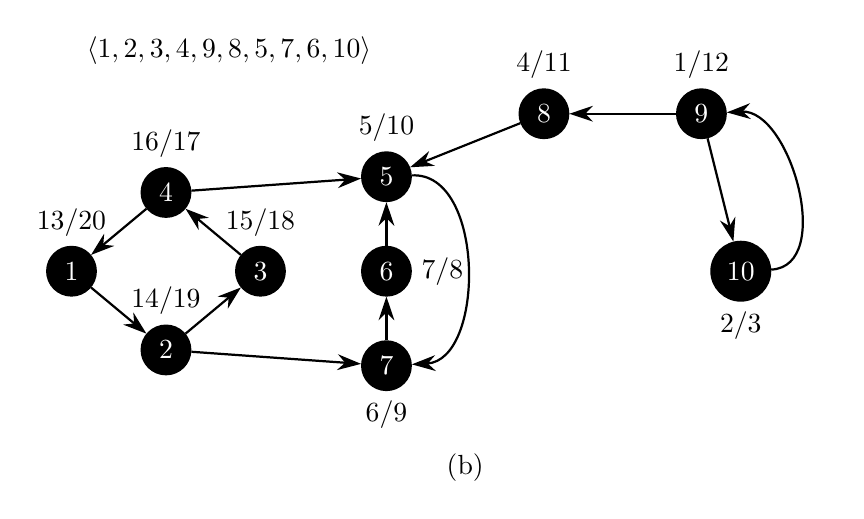
\begin{tikzpicture}
    %comp 1
    \node[mynode, label=above:{$13/20$}, fill=black](n1) at (0,0){\textcolor{white}{1}};
    \node[mynode, label=above:{$14/19$}, fill=black](n2) at (1.2,-1){\textcolor{white}{2}};
    \node[mynode, label=above:{$16/17$}, fill=black](n3) at (1.2, 1){\textcolor{white}{4}};
    \node[mynode, label=above:{$15/18$}, fill=black](n4) at (2.4, 0){\textcolor{white}{3}};
    \draw[myarrow](n1)--(n2);
    \draw[myarrow](n3)--(n1);
    \draw[myarrow](n4)--(n3);
    \draw[myarrow](n2)--(n4);
    %comp 2
    \node[mynode, label=above:{$5/10$}, fill=black](n5) at (4,1.2){\textcolor{white}{5}};
    \node[mynode, label=right:{$7/8$}, fill=black](n6) at (4,0){\textcolor{white}{6}};
    \node[mynode, label=below:{$6/9$}, fill=black](n7) at (4, -1.2){\textcolor{white}{7}};
    \draw[myarrow](n6) -- (n5);
    \draw[myarrow](n5) to[out=3,in=3] (n7);
    \draw[myarrow](n7) -- (n6);

    %comp edges
    \draw[myarrow](n3) -- (n5);
    \draw[myarrow](n2) -- (n7);
    %comp 3
    \node[mynode, label=above:{$4/11$}, fill=black](n8) at (6, 2){\textcolor{white}{8}};
    %comp 4
    \node[mynode, label=above:{$1/12$}, fill=black](n9) at (8, 2){\textcolor{white}{9}};
    \node[mynode, label=below:{$2/3$}, fill=black](na) at (8.5, 0){\textcolor{white}{10}};
    \draw[myarrow](n9) -- (n8);
    \draw[myarrow](na) to[out=3,in=3] (n9);
    \draw[myarrow](n9) -- (na);
    \draw[myarrow](n8) -- (n5);

    % label for the second graph
    \node[align=center, xshift=2cm, yshift=2.8cm] (label2) {$\langle 1, 2, 3, 4, 9, 8, 5, 7, 6, 10 \rangle$};
    \node[below=10mm] at (5, -1.2) {(b)};
\end{tikzpicture}}
    \resizebox{!}{4cm}{
        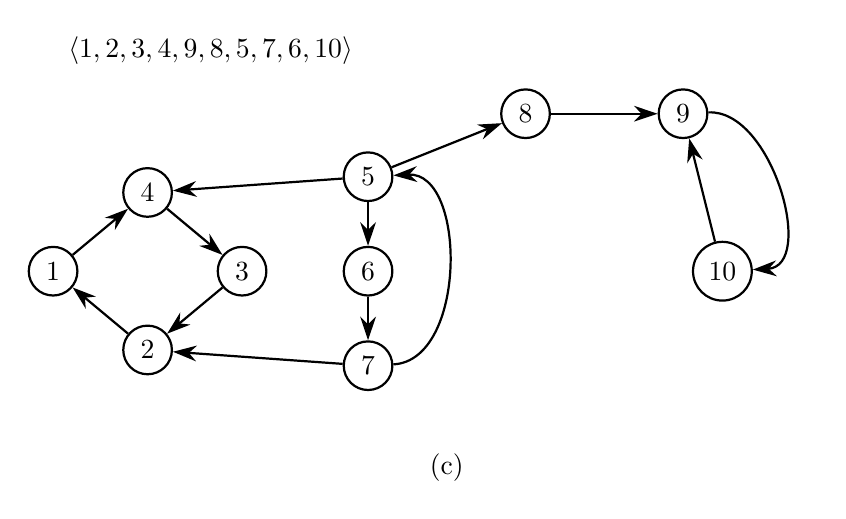
\begin{tikzpicture}
    %comp 1
    \node[mynode](n1) at (0,0){1};
    \node[mynode](n2) at (1.2,-1){2};
    \node[mynode](n4) at (1.2, 1){4};
    \node[mynode](n3) at (2.4, 0){3};
    \draw[myarrow](n2)--(n1);
    \draw[myarrow](n1)--(n4);
    \draw[myarrow](n4)--(n3);
    \draw[myarrow](n3)--(n2);
    %comp 2
    \node[mynode](n5) at (4,1.2){5};
    \node[mynode](n6) at (4,0){6};
    \node[mynode](n7) at (4, -1.2){7};
    \draw[myarrow](n5) -- (n6);
    \draw[myarrow](n7) to[out=3,in=3] (n5);
    \draw[myarrow](n6) -- (n7);

    %comp edges
    \draw[myarrow](n5) -- (n4);
    \draw[myarrow](n7) -- (n2);
    %comp 3
    \node[mynode](n8) at (6, 2){8};
    %comp 4
    \node[mynode](n9) at (8, 2){9};
    \node[mynode](na) at (8.5, 0){10};
    \draw[myarrow](n8) -- (n9);
    \draw[myarrow](n9) to[out=3,in=3] (na);
    \draw[myarrow](na) -- (n9);
    \draw[myarrow](n5) -- (n8);

    \node[align=left, xshift=2cm, yshift=2.8cm] (label2) {$\langle 1, 2, 3, 4, 9, 8, 5, 7, 6, 10 \rangle$};
    \node[below=10mm] at (5, -1.2) {(c)};
\end{tikzpicture} \quad \quad \quad
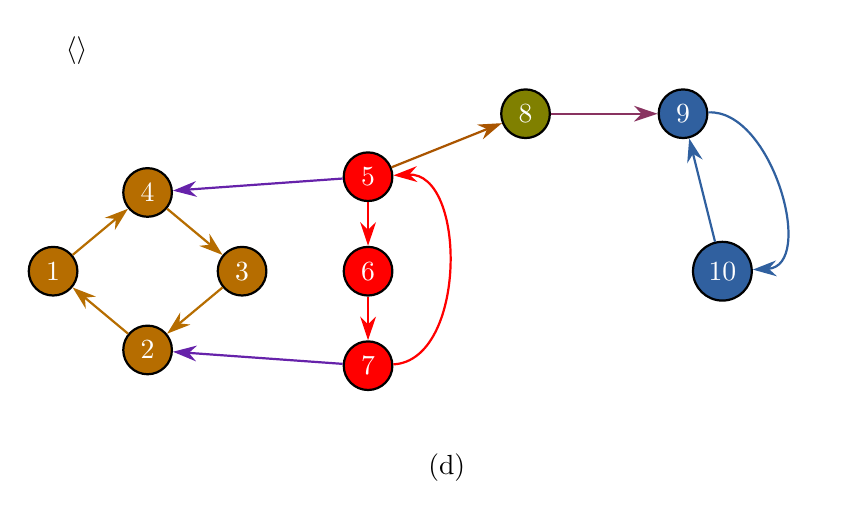
\begin{tikzpicture}
    %comp 1
    \node[mynode, fill={rgb:red,4;green,2;yellow,1}](n1) at (0,0){\textcolor{white}{1}};
    \node[mynode, fill={rgb:red,4;green,2;yellow,1}](n2) at (1.2,-1){\textcolor{white}{2}};
    \node[mynode, fill={rgb:red,4;green,2;yellow,1}](n4) at (1.2, 1){\textcolor{white}{4}};
    \node[mynode, fill={rgb:red,4;green,2;yellow,1}](n3) at (2.4, 0){\textcolor{white}{3}};
    \draw[myarrow, color={rgb:red,4;green,2;yellow,1}](n2)--(n1);
    \draw[myarrow, color={rgb:red,4;green,2;yellow,1}](n1)--(n4);
    \draw[myarrow, color={rgb:red,4;green,2;yellow,1}](n4)--(n3);
    \draw[myarrow, color={rgb:red,4;green,2;yellow,1}](n3)--(n2);
    %comp 2
    \node[mynode, fill=red](n5) at (4,1.2){\textcolor{white}{5}};
    \node[mynode, fill=red](n6) at (4,0){\textcolor{white}{6}};
    \node[mynode, fill=red](n7) at (4, -1.2){\textcolor{white}{7}};
    \draw[myarrow, red](n5) -- (n6);
    \draw[myarrow, red](n7) to[out=3,in=3] (n5);
    \draw[myarrow, red](n6) -- (n7);
    %comp edges
    \draw[myarrow, color={rgb:red,1;blue,2}](n5) -- (n4);
    \draw[myarrow, color={rgb:red,1;blue,2}](n7) -- (n2);
    %comp 3
    \node[mynode, fill=green!50!red](n8) at (6, 2){\textcolor{white}{8}};
    %comp 4
    \node[mynode, fill={rgb:red,1;green,2;blue,5}](n9) at (8, 2){\textcolor{white}{9}};
    \node[mynode, fill={rgb:red,1;green,2;blue,5}](na) at (8.5, 0){\textcolor{white}{10}};
    \draw[myarrow, color={rgb:red,4;green,1;blue,3}](n8) -- (n9);
    \draw[myarrow, color={rgb:red,1;green,2;blue,5}](n9) to[out=3,in=3] (na);
    \draw[myarrow, color={rgb:red,1;green,2;blue,5}](na) -- (n9);
    \draw[myarrow, color={rgb:red,2;green,1}](n5) -- (n8);

    \node[align=left, xshift=0.3cm, yshift=2.8cm] (label2) {$\langle \rangle$};

    \node[below=10mm] at (5, -1.2) {(d)};
\end{tikzpicture}}
    \caption{Esempio di esecuzione dell'algoritmo di Kosaraju su un grafo diretto}
    \label{fig:kozaraju_example}
\end{figure}

In figura~\ref{fig:kozaraju_example} sono rappresentate le fasi rilevanti dell'algoritmo di Kozaraju
applicato al grafo in (a).
In (b) \`e rappresentato lo stato del grafo al termine della procedura DFS, assieme alla lista dei nodi ordinata
per tempi di fine visita.
In (c) il grafo trasposto ottenuto invertendo gli archi del grafo in (a).
In (d) lo stato del grafo trasposto in (c) al termine della seconda procedura di visita in
profondit\`a, dove colori dello stesso colore rappresentano nodi appartenenti alla stessa componente fortemente
connessa fornita in output.

\nlparagraph{Complessit\`a}

L'algoritmo di Kosaraju ha una complessit\`a temporale di $\Theta(V + E)$, in quanto:
\begin{itemize}
    \item A riga 1 viene eseguita una ricerca in profondit\`a tradizionale, quindi con costo $\Theta(|V| + |E|)$.
    \item A riga 2 viene costruito il grafo trasposto $G^T$ e come gi\`a detto, la sua costruzione pu\`o avvenire in
    un tempo $\Theta(|V| + |E|)$, iterando prima sull'insieme dei nodi di $G$ e poi sui suoi archi, invertendone
    l'orientamento.
    \item L'ordinamento dei nodi di $G^T$ pu\`o essere realizzato nel corso della visita a riga 1 attraverso la
    costruizione di una lista concatenata, per cui i singoli nodi possono essere aggiunti in testa alla lista nel
    momento in cui vengono colorati di nero, in tempo costante, per un totale di $\Theta(|V|)$, e non ci sono costi
    aggiuntivi per la costruzione dell'ordinamento.
    \item A riga 3 viene eseguita la procedura DFS che corrisponde ad una visita in profondit\`a di $G^T$, quindi
    sempre di complessit\`a $\Theta(|V| + |E|)$.
\end{itemize}

\subsection{Enumerazione di cricche}\label{sec:enumerazione-di-cricche}

Come gi\`a discusso, una cricca di un grafo \`e un sottoinsieme di nodi che sono tutti mutuamente
adiacenti, ovvero un sottoinsieme di nodi che formano un sottografo completo.
Nella teoria dei grafi, il concetto di cricca \`e normalmente riferito al contesto di un grafo non orientato,
in cui \`e sufficiente un singolo arco non orientato $\{u, v\}$ per rendere i due nodi $u$ e $v$ tra loro
mutualmente adiacienti.
Tuttavia il concetto di cricca pu\`o essere esteso anche al contesto di grafi orientati: in particolare \'e sempre
possibile considerare la versione non orientata alla base di un grafo orientato secondo due possibili modalit\`a:
\begin{itemize}
    \item Rimuovendo l'orientamento degli archi: in questo caso, \`e sufficiente un singolo arco orientato $(u, v)$
        per avere un arco non orientato ${u, v}$ nella versione non orientata, rendendo quindi i nodi $u$ e $v$ tra loro
        mutuamente adiacienti anche se ci\`o non fosse vero nella versione orientata originale.
    \item Considerando come archi non diretti le relazioni simmetriche di adiacienza tra i nodi del grafo orientato
        originale: in questo caso, la versione non orientata conterr\`a un arco non diretto ${u, v}$ se e solo se
        nel grafo orientato originale esistono entrambi gli archi $(u, v)$ e $(v, u)$.
\end{itemize}

\begin{figure}[H]
    \centering
    \begin{tikzpicture}
    % Define the nodes
    \node[mynode] (1) at (0, 0) {$v_1$};
    \node[mynode] (2) at (1.5, 1.5) {$v_2$};
    \node[mynode] (3) at (3, 0) {$v_3$};
    \node[mynode] (4) at (1.5, -1.5) {$v_4$};

    \node[] (a) [below of=4, node distance=1cm] {(a)};

    % Draw the edges
    \draw[myarrow] (1) -- (2);
    \draw[myarrow] (2) to[out=180, in=90] (1);
    \draw[myarrow] (4) to[out=225, in=135, looseness=5] (4); % This edge is a self-loop, corrected below
    \draw[myarrow] (2) -- (3);
    \draw[myarrow] (3) -- (4);
    \draw[myarrow] (3) -- (1);

    \begin{scope}[shift={(5,0)}]
        % Define the nodes
    \node[mynode] (1) at (0, 0) {$v_1$};
    \node[mynode] (2) at (1.5, 1.5) {$v_2$};
    \node[mynode] (3) at (3, 0) {$v_3$};
    \node[mynode] (4) at (1.5, -1.5) {$v_4$};

    % Draw the edges
    \draw[edge, thick] (1) -- (2);
    \draw[edge, thick] (2) -- (3);
    \draw[edge, thick] (3) -- (4);
    \draw[edge, thick] (3) -- (1);

    \node[] (b) [below of=4, node distance=1cm] {(b)};

    \end{scope}

    \begin{scope}[shift={(10,0)}]
        % Define the nodes
    \node[mynode] (1) at (0, 0) {$v_1$};
    \node[mynode] (2) at (1.5, 1.5) {$v_2$};
    \node[mynode] (3) at (3, 0) {$v_3$};
    \node[mynode] (4) at (1.5, -1.5) {$v_4$};

    % Draw the edges
    \draw[edge, thick] (1) -- (2);

    \node[] (c) [below of=4, node distance=1cm] {(c)};

    \end{scope}
\end{tikzpicture}
    \caption{Esempio di grafo orientato e delle sue due possibili versioni non orientate}
    \label{fig:undirected_version_example}
\end{figure}

La definizione di cricca in un grafo diretto pu\`o quindi essere declinata in due modi a seconda di quanto si vuole
rendere lasco il concetto di adiacienza tra i nodi.
In figura~\ref{fig:undirected_version_example} sono rappresentati in (a) un grafo diretto, in (b) la sua versione non
diretta ottenuta rimuovendo l'orientamento degli archi e in (c) quella ottenuta considerando come archi non diretti le
relazioni simmetriche di adiacienza tra i nodi. \`E utile notare che la versione non orientata (b) \`e mantenuta come
grafo semplice, ovvero un grafo non orientato che non contiene archi multipli o cappi.
Appare evidente di come la versione non orientata (c) sia pi\`u restrittiva rispetto alla versione (b): mentre
in (b) le cricche di dimensione superiore a uno sono $\{v_1, v_2, v_3\}$ e $\{v_3, v_4\}$, in (c) l'unica
cricca di dimensione superiore a uno \`e $\{v_1, v_2\}$. \newline

D'ora in avanti, quando si far\`a riferimento al concetto di cricca nel contesto di grafo diretto, si far\`a
uso dell'espressione \textit{cricca non reciproca} per indicare le cricche presenti nella versione non diretta
ottenuta rimuovendo semplicemente l'orientamento degli archi, come in (b), e \textit{cricca reciproca} per indicare
le cricche presenti nella versione non diretta ottenuta considerando le relazioni simmetriche di adiacienza tra i nodi,
come in (c).


\nlparagraph{Algoritmo di Bron-Kerbosch}

L'algoritmo di Bron-Kerbosch, descritto per la prima volta in nel 1973~\cite{10.1145/362342.362367} da
Coen Bron e Joep Kerbosch, \`e un noto algoritmo per l'enumerazione delle cricche massimali in grafi non diretti.
Con cricche massimali si intendono cricche che non possono essere estese aggiungendo ulteriori nodi senza
violare la propriet\`a di cricca, ovvero cricche che non sono sottoinsieme proprio di altre cricche presenti nel grafo.
Nella sua versione con pivoting (talvolta chiamata ``Tomita''), si tratta dell'algoritmo esatto considerato essere
pi\`u efficiente nelle applicazioni pratiche rispetto ad altri algoritmi per l'enumerazione di cricche, oltre che
essere stato dimostrato ottimale rispetto al numero massimo di cricche presenti in un grafo~\cite{TOMITA200628}.
\newline

L'algoritmo si basa su un approccio ricorsivo di backtracking, in cui a partire da un insieme vuoto di nodi, si
cerca di costruire una cricca massimale aggiungendo nodi uno alla volta, valutando solo i nodi che
possono essere aggiunti alla cricca senza violare la propriet\`a di cricca.
A partire dalla cricca corrente, ovvero la cricca attualmente in costruzione, ad ogni chiamata ricorsiva si valuta
la scelta di aggiungere un nodo valido tra quelli disponibili, scendendo in profondit\`a nell'albero della ricorsione.
Al termine della chiamata riscorsiva, il nodo viene inserito in un insieme dei nodi
gi\`a considerati, corrispondente alla scelta di escludere tale nodo dalla costruzione della cricca corrente in tutte
le chiamate successive. \newline

\begin{algorithm}[H] \floatname{algorithm}{Algoritmo}
    \caption{BRON-KERBOSH($R$, $P$, $X$)}\label{alg:bk1}
    \begin{algorithmic}[1]
        \If {$P \cup X$ $=$ $\emptyset$}
            \State Fornisci in output $R$ come una cricca massimale
        \Else

            \For{$v\in P$}
                \State BRON-KERBOSH($R \cup \{v\},$ $P \cap N(v)$, $X \cap N(v)$)
                \State $P:= P \setminus \{v\}$
                \State $X:= X \cup \{v\}$
            \EndFor
        \EndIf
    \end{algorithmic}
\end{algorithm}

Nello pseudocodice, la notazione $N(v)$ indica l'insieme dei vicini del nodo $v$, ovvero l'insieme dei nodi adiacenti
a $v$ tramite un arco non orientato.
Nel corso della sua esecuzione, quindi, l'algoritmo manipola tre insiemi di nodi disgiunti che vengono passati
alle procedure ricorsive, che sono:
\begin{itemize}
    \item $R$: cricca correntemente in costruzione
    \item $P$: insieme di nodi adiacienti ad ogni nodo in $R$, ovvero i nodi candidati a far parte della cricca corrente
    non ancora considerati nella costruzione di una cricca massimale che includa $R$.
    \item $X$: insieme di nodi adiacienti ad ogni nodo in $R$, gi\`a considerati nella costruzione di una cricca
    massimale che includa $R$.
\end{itemize}

\begin{figure}[H]
    \centering
    \resizebox{!}{10cm}{
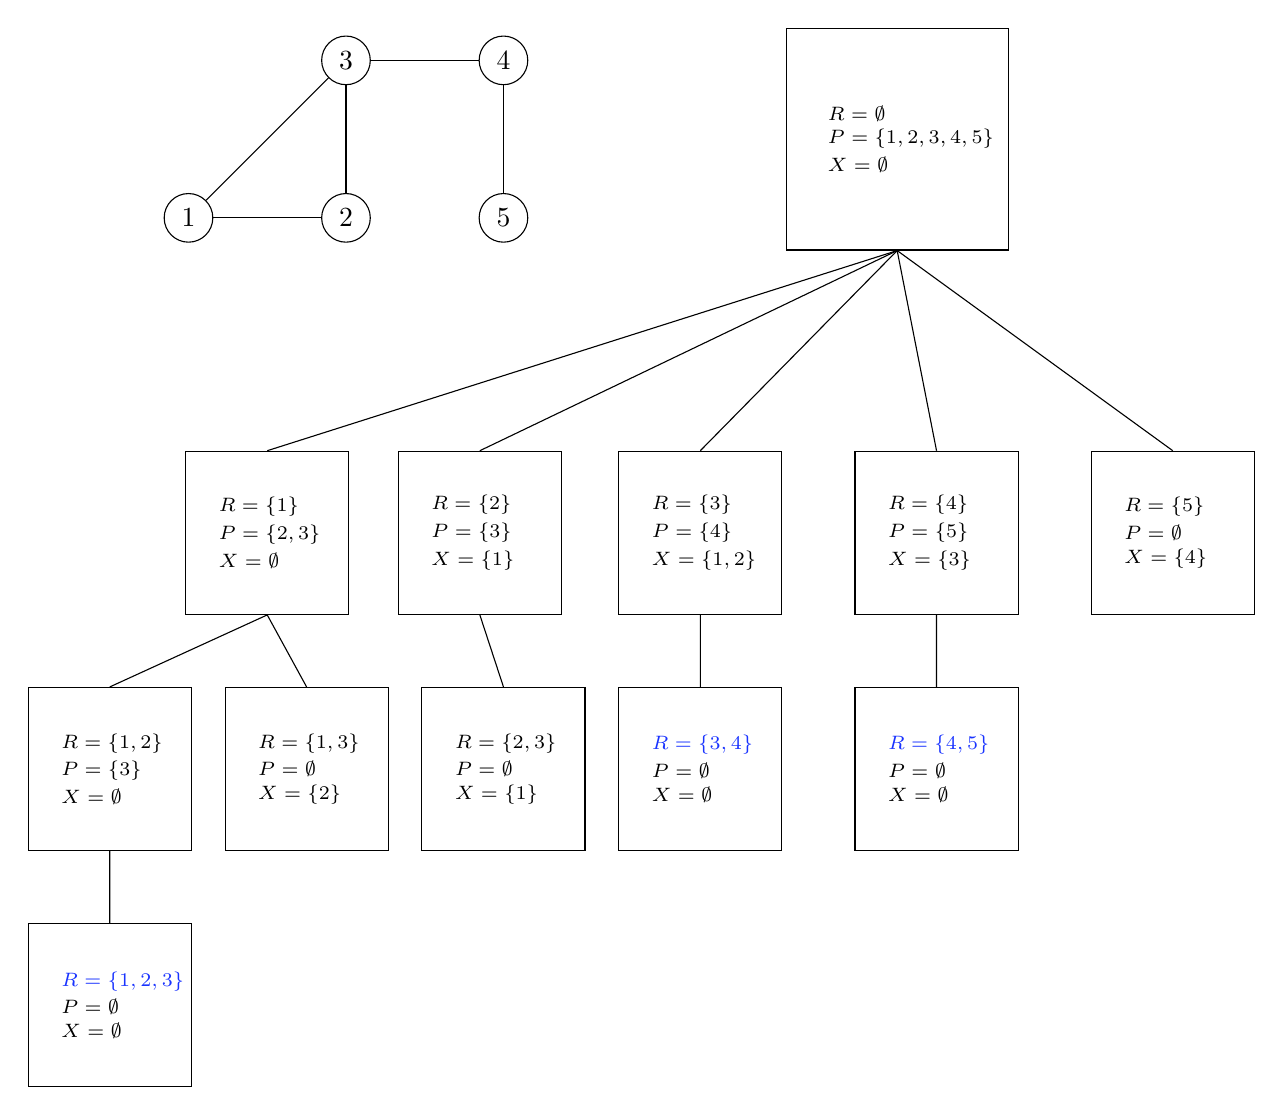
\begin{tikzpicture}[square/.style={regular polygon,regular polygon sides=4}]
	    %H0
	    \node (A) at (-1,2) [font=\scriptsize, text width=5em,square,draw]
	    	{\shortstack[l]{$ R=\emptyset$\\$P=\{1,2,3,4,5\}$\\$X=\emptyset$}};

	    %H1
	    \node (B) at (-9, -3) [font=\scriptsize, text width=3.5em,square,draw]
	    	{\shortstack[l]{$ R=\{1\}$\\$P=\{2,3\}$\\$X=\emptyset$}};

	    \node (C) at (-6.3, -3) [font=\scriptsize, text width=3.5em,square,draw]
	    	{\shortstack[l]{$ R=\{2\}$\\$P=\{3\}$\\$X=\{1\}$}};

	    \node (D) at (-3.5, -3) [font=\scriptsize, text width=3.5em,square,draw]
	    	{\shortstack[l]{$ R=\{3\}$\\$P=\{4\}$\\$X=\{1,2\}$}};

	    \node (E) at (-0.5, -3) [font=\scriptsize, text width=3.5em,square,draw]
		{\shortstack[l]{$ R=\{4\}$\\$P=\{5\}$\\$X=\{3\}$}};

	    \node (F) at (2.5, -3) [font=\scriptsize, text width=3.5em,square,draw]
		{\shortstack[l]{$R=\{5\}$\\$P=\emptyset$\\$X=\{4\}$}};
	    % H2
	    \node (G) at (-11 , -6) [font=\scriptsize, text width=3.5em,square,draw]
	    	{\shortstack[l]{$ R=\{1,2\}$\\$P=\{3\}$\\$X=\emptyset$}};

	    \node (H) at (-8.5 , -6) [font=\scriptsize, text width=3.5em,square,draw]
	    	{\shortstack[l]{$ R=\{1,3\}$\\$P=\emptyset$\\$X=\{2\}$}};

	    \node (I) at (-6 , -6) [font=\scriptsize, text width=3.5em,square,draw]
	    	{\shortstack[l]{$ R=\{2,3\}$\\$P=\emptyset$\\$X=\{1\}$}};

	    \node (J) at (-3.5 , -6) [font=\scriptsize, text width=3.5em,square,draw]
	    	{\shortstack[l]{$ \color{blue}R=\{3,4\}$\\$P=\emptyset$\\$X=\emptyset$}};

	    \node (K) at (-0.5 , -6) [font=\scriptsize, text width=3.5em,square,draw]
	    	{\shortstack[l]{$ \color{blue}R=\{4,5\}$\\$P=\emptyset$\\$X=\emptyset$}};
	    %H3
	    \node (L) at (-11 , -9) [font=\scriptsize, text width=3.5em,square,draw]
	    	{\shortstack[l]{$ \color{blue}R=\{1,2,3\}$\\$P=\emptyset$\\$X=\emptyset$}};
	    %H3

	    % E0-1
	    \draw (A) to[out=270, in=90, looseness=0] (B);
	    \draw (A) to[out=270, in=90, looseness=0] (C);
	    \draw (A) to[out=270, in=90, looseness=0] (D);
	    \draw (A) to[out=270, in=90, looseness=0] (E);
	    \draw (A) to[out=270, in=90, looseness=0] (F);
	    % E1-2
	    \draw (B) to[out=270, in=90, looseness=0] (G);
	    \draw (B) to[out=270, in=90, looseness=0] (H);
	    \draw (C) to[out=270, in=90, looseness=0] (I);
	    \draw (D) to[out=270, in=90, looseness=0] (J);
	    \draw (E) to[out=270, in=90, looseness=0] (K);

	    % E2-3

	    \draw (G) -- (L);

	\begin{scope}[shift={(-10, 1)}]
		\node[circle, draw] (A) {1};
		\node[circle, draw] (B) [right of=A, node distance=2cm] {2};
		\node[circle, draw] (C) [above of=B, node distance=2cm] {3};
		\node[circle, draw] (D) [right  of=C, node distance=2cm] {4};
		\node[circle, draw] (E) [below of=D, node distance=2cm] {5};

		\draw(A) -- (B);
		\draw(B) -- (C);
		\draw(A) -- (C);
		\draw(C) -- (D);
		\draw(D) -- (E);
	\end{scope}
\end{tikzpicture}
}
    \caption{Esempio di albero di ricorsione dell'algoritmo di Bron-Kerbosch}
    \label{fig:bron_kerbosh_tree_example}
\end{figure}

Inizialmente gli insiemi $R$ e $X$ sono vuoti, mentre $P$ contiene tutti i nodi del grafo.
Le chiamate ricorsive valutano l'aggiunta di nodi da $P$ in $R$, e gli insiemi $P$ e $X$ vengono aggiornati
mantenendo solo nodi che sono adiacenti a tutti i nodi in $R$, e che quindi, presi singolarmente, potrebbero
essere aggiunti alla cricca corrente senza violarne la propriet\`a di cricca.
Quando $P$ \'e vuoto, le chiamate ricorsive nel ramo corrente della ricorsione terminano e, a quel punto,
$R$ rappresenter\'a una cricca.
Tuttavia l'algoritmo riconosce se tale cricca sia massimale o meno valutando se al contempo l'insieme $X$ sia,
rispettivamente, vuoto o non vuoto.
Si noti infatti che un insime $X$ non vuoto indicherebbe che la cricca corrente potrebbe essere estesa aggiungendo
nodi in $X$, concludendo non solo che la cricca in $R$ non \'e massimale, ma anche che la cricca massimale che
la contiene assieme ai nodi in $X$ \'e gi\`a stata trovata. \newline

\nlparagraph{Algoritmo Tomita}
Bron e Kerbosch proposero nel loro articolo orginale una versione migliorata del loro algoritmo, la quale
prevede l'utilizzo di una strategia di pivoting, che permette di ridurre le chiamate ricorsive della procedura
trovando comunque tutte le cricche massimali.

\begin{algorithm} \floatname{algorithm}{Algoritmo}
    \caption{BRON-KERBOSH-PIVOT($R$, $P$, $X$, $T$)}\label{alg:bk2}
    \begin{algorithmic}[1]
        \If {$P \cup X$ $=$ $\emptyset$}
            \State Fornisci in output $R$ come una cricca massimale
        \Else
            \State Scegli un nodo pivot $u\in P\cup X$ t. c. $|P \cap N(u)|$ = $max_{v \in P \cup X}|P \cap N(v)|$
            \For{$v\in P \setminus N(u)$}
                \State BRON-KERBOSH-PIVOT($R \cup \{v\},$ $P \cap N(v)$, $X \cap N(v)$)
                \State $P:=P \setminus \{v\}$
                \State $X:=X \cup \{v\}$
            \EndFor
        \EndIf
    \end{algorithmic}
\end{algorithm}

In particolare, ad ogni procedura ricorsiva BRON-KERBOSCH-PIVOT si sceglie un nodo pivot $u \in P$.
Le chiamate ricorsive effettuate sull'insieme $P$ saranno quindi ristrette ai nodi in $P$ che non sono vicini di $u$,
quindi $u$ stesso e tutti i suoi non-vicini in $P$.
Sebbene qualunque nodo in $P$ possa essere scelto come pivot, come dimostrato da Tomita~\cite{TOMITA200628},
la scelta migliore del pivot ricade sul nodo che abbia il maggior numero di vicini in $P$, scelta che di fatto
permette di escludere il maggior numero di elementi da $P$ e, quindi, di evitare il maggior numero di chiamate ricorsive.
Per questo motivo, questa versione dell'algoritmo di Bron-Kerbosch viene spesso chiamata \textit{Tomita}. \newline

La tecnica del pivoting nasce dalla considerazione per cui la procedura ricorsiva applicata aggiungendo un arbitrario
nodo $u$ a $R$ permette comunque a tutti i suoi vicini di poter essere aggiunti a $R$ tramite le sotto-chiamate
ricorsive immediatamene successive.
In altre parole, i vicini di $u$ in $P$ faranno parte di ogni cricca massimale che
contenga $R$ che ammette anche $u$, in quanto ogni nodo in $P$ preso singolarmente \'e adiacente ad ogni nodo in $R$.
\newline

\begin{figure}[H]
    \centering
    \newcommand{\nodestar}[6]{
    \node[draw, circle] (#1a) at (#2, #3) [opacity=0] {}; \draw (#1) -- (#1a);
    \node[draw, circle] (#1b) at (#2, #4) [opacity=0] {}; \draw (#1) -- (#1b);
    \node[draw, circle] (#1c) at (#2, #5) [opacity=0] {}; \draw (#1) -- (#1c);
    \node[draw, circle] (#1d) at (#2, #6) [opacity=0] {}; \draw (#1) -- (#1d);
}

\begin{tikzpicture}
    \node (R) at (1.5, 2) {$R$}
    \node[draw, circle] (1) at (0, 1) {$v_1$};
    \node[draw, circle] (2) at (0.5, -1.5) {$v_2$};
    \node[draw, circle] (3) at (2.5, -1) {$v_3$};
    \node[draw, circle] (4) at (3, 1.5) {$v_4$};
    \draw (1) -- (2);
    \draw (1) -- (3);
    \draw (1) -- (4);
    \draw (2) -- (3);
    \draw (2) -- (4);
    \draw (3) -- (4);

    \node (P) at (6, 2) {$P$}
    \node[draw, circle, blue] (u) at (5, 1.5) {$u$}; \nodestar{u}{4}{1.6}{1.4}{1.2}{1}
    \node[draw, circle, red] (5) at (4.5, 0) {$v_5$}; \nodestar{5}{3.5}{0.4}{0.2}{0}{-0.2}
    \node[draw, circle, red] (6) at (5.5, 0.2) {$v_6$}; \nodestar{6}{4.5}{0.3}{0.1}{-0.1}{-0.3}
    \node[draw, circle, red] (7) at (6.5, 0.7) {$v_7$}; \nodestar{7}{5.5}{0.8}{0.6}{0.4}{0.2}
    \node[draw, circle, red] (8) at (7.5, 1.1) {$v_8$}; \nodestar{8}{6.5}{1.2}{1}{0.8}{0.6}
    \node[draw, circle, blue] (9) at (4.5, -1) {$v_9$}; \nodestar{9}{3.5}{-0.6}{-0.8}{-1}{-1.2}
    \node[draw, circle, blue] (10) at (5.5, -1) {$v_{10}$}; \nodestar{10}{4.5}{-0.6}{-0.8}{-1}{-1.2}
    \node[draw, circle, blue] (11) at (6.5, -1) {$v_{11}$}; \nodestar{11}{5.5}{-0.6}{-0.8}{-1}{-1.2}
    \node[draw, circle, blue] (12) at (7.5, -1) {$v_{12}$}; \nodestar{12}{6.5}{-0.6}{-0.8}{-1}{-1.2}

    \draw (u) -- (5);
    \draw (u) -- (6);
    \draw (u) -- (7);
    \draw (u) -- (8);

    \node (X) at (9.5, 2) {$X$}
    \node[draw, circle] (13) at (9.5, 1.2) {$v_{13}$}; \nodestar{13}{8.5}{1.4}{1.2}{1}{0.8}
    \node[draw, circle] (14) at (9.5, 0.2) {$v_{14}$}; \nodestar{14}{8.5}{0.4}{0.2}{0}{-0.2}
    \node[draw, circle] (15) at (9.5, -0.8) {$v_{15}$}; \nodestar{15}{8.5}{-0.3}{-0.5}{-0.7}{-0.9}
\end{tikzpicture}
    \caption{Rappresentazione dei tre insiemi $R$, $P$ e $X$ nel corso dell'algoritmo di Bron-Kerbosch con pivoting}
    \label{fig:bron_kerbosh_pivot_example}
\end{figure}

La figura~\ref{fig:bron_kerbosh_pivot_example} tenta di dare un'idea migliore degli insiemi R, P ed X nel corso
dell'esecuzione dell'algoritmo con strategia di pivoting.
Il nodo $u$ \'e scelto come pivot, e le chiamate ricorsive al livello corrente della ricorsione sono limitate ai nodi
in blu.
I segmenti uscenti da ogni nodo in P ed X rappresentano gli archi che li rendono adiacienti ad ogni nodo in R.

\begin{figure}[H]
    \centering
    \resizebox{!}{10cm}{
\begin{tikzpicture}[square/.style={regular polygon,regular polygon sides=4}]
	    %H0
	    \node (A) at (-9.15,1.4) [font=\scriptsize, text width=4em,square,draw]
	    	{\shortstack[l]{$Pivot=3$\\$ R=\emptyset$\\$P=\{1,2,3,4\}$\\$X=\emptyset$}};
	    %H1
	    \node (B) at (-11.5,-2.8) [font=\scriptsize, text width=4em,square,draw]
	    	{\shortstack[l]{$Pivot=1$\\$ R=\{3\}$\\$P=\{1,2,4\}$\\$X=\emptyset$}};

	    \node (C) at (-6.5,-2.8) [font=\scriptsize, text width=4em,square,draw]
	    	{\shortstack[l]{$Pivot=4$\\$ R=$\{5\}\\$P=\{4\}$\\$X=\emptyset$}};
            %H2
	    \node (D) at (-13,-6) [font=\scriptsize, text width=4em,square,draw]
	    	{\shortstack[l]{$Pivot=2$\\$ R=$\{3,1\}\\$P=\{2\}$\\$X=\emptyset$}};
	    \node (E) at (-10,-6) [font=\scriptsize, text width=4em,square,draw]
	    	{\shortstack[l]{$\color{blue}R=$\color{blue}\{3,4\}\\$P=\emptyset$\\$X=\emptyset$}};

	    \node (F) at (-6.5,-6) [font=\scriptsize, text width=4em,square,draw]
	    	{\shortstack[l]{$\color{blue}R=$\color{blue}\{5,4\}\\$P=\emptyset$\\$X=\emptyset$}};
	    %H4
	    \node (G) at (-13, -9) [font=\scriptsize, text width=4em,square,draw]
	    	{\shortstack[l]{$\color{blue}R=$\color{blue}\{3,1,2\}\\$P=\emptyset$\\$X=\emptyset$}};



	    %E0-1
	    \draw (A) to[out=270, in=90, looseness=0] (B);
	    \draw (A) to[out=270, in=90, looseness=0] (C);

	    %E1-2
	    \draw (B) to[out=270, in=90, looseness=0] (D);
	    \draw (B) to[out=270, in=90, looseness=0] (E);
	    \draw (C) to[out=270, in=90, looseness=0] (F);

	    %E2-3
	    \draw (D) to[out=270, in=90, looseness=0] (G);

	\begin{scope}[shift={(-16.5, 0.3)}]
		\node[circle, draw] (A) {1};
		\node[circle, draw] (B) [right of=A, node distance=2cm] {2};
		\node[circle, draw] (C) [above of=B, node distance=2cm] {3};
		\node[circle, draw] (D) [right  of=C, node distance=2cm] {4};
		\node[circle, draw] (E) [below of=D, node distance=2cm] {5};

		\draw(A) -- (B);
		\draw(B) -- (C);
		\draw(A) -- (C);
		\draw(C) -- (D);
		\draw(D) -- (E);
	\end{scope}
\end{tikzpicture}
}
    \caption{Esempio di albero di ricorsione dell'algoritmo di Bron-Kerbosch con pivoting}
    \label{fig:bron_kerbosh_pivot_tree_example}
\end{figure}

La figura ~\ref{fig:bron_kerbosh_pivot_tree_example} mostra l'albero di ricorsione derivante dall'applicazione
dell'algoritmo di Bron-Kerbosch con pivoting sullo stesso grafo orientato presente in figura
~\ref{fig:bron_kerbosh_tree_example}, rendendo evidente come la strategia di pivoting permetta di ridurre il numero
di chiamate ricorsive rispetto alla versione senza pivoting.

\nlparagraph{Complessit\'a}

Come dimostrato da Tomita ~\cite{TOMITA200628}, adottando una strategia di pivoting affinch\'e si scelga il nodo pivot
$w$ con il maggior numero di vicini in $P$, l'algoritmo di Bron-Kerbosch ha una complessit\'a temporale pari a
$O(3^{n/3})$, che \'e una complessit\'a ottimale, in quanto il numero massimo di cricche massimali che si possono
trovare in un grafo con $n$ nodi \'e dimostrato essere $3^{n/3}$.

\subsection{Enumerazione di circuiti semplici}\label{sec:enumerazione-di-cicli}

Come gi\`a spiegato nel capitolo introduttivo, un circuito semplice di un grafo diretto \'e un circuito
che non contiene nodi ripetuti, ad eccezione del nodo di partenza e di arrivo.
Dal momento in cui, per definizione, un circuito non pu\`o contenere archi ripetuti, parlare anche solo di cicli
semplici garantirebbe che esso non contenga neanche archi ripetuti.
Si potrebbe notare che, mentre componenti fortemente connesse e cricche sono concetti che possono essere
ricondotti ad un insieme non ordinato, i circuiti semplici comprendono in s\'e una sequenza di nodi in un determinato
ordine.
Per questo motivo diventa rilevante distinguere tra cicli e permutazioni cicliche, in quanto ogni ciclo
pu\`o essere rappresentato da un insieme di permutazioni cicliche.
Ad esempio, il ciclo $c_1 = \langle v_1, v_2, v_3, v_1 \rangle$ pu\`o essere rappresentato anche attraverso le
permutazioni cicliche $\langle v_2, v_3, v_1, v_2 \rangle$ e $\langle v_3, v_1, v_2, v_3 \rangle$, in quanto entrambe
rappresentano lo stesso anello di nodi percorsi nello stesso senso. \newline
\`E interessante notare che il ciclo $c_2 = \langle v_1, v_3, v_2, v_1 \rangle$, nonostante sia un ciclo semplice
composto degli stessi nodi di $c_1$, non pu\`o essere rappresentato da nessuna permutazione ciclica di $c_1$.
Per questo motivo due cicli si dicono distinti se non sono l'uno una permutazione ciclica dell'altro. \newline

In questa sezione tratteremo, quindi, un algoritmo per l'enumerazione di circuiti semplici in un grafo diretto, che
risolve il problema di individuare tutti i cicli semplici distinti presenti in un grafo diretto.


\nlparagraph{Algoritmo di ricerca dei circuiti semplici di Johnson}
L'algoritmo per la ricerca dei circuiti semplici di Donald B. Johnson, proposto nel 1975~\cite{doi:10.1137/0204007},
provvede ad enumerare tutti i cicli in un grafo orientato eseguendo delle visite in profondit\`a. \newline

A partire da un ordinamento arbitrario dei nodi, l'algoritmo esegue la procedura di visita ricorsiva CIRCUIT partendo
da ciascuno di essi, individuando di volta in volta tutti e soli i circuiti semplici contenenti il nodo di partenza $s$.
Nel corso di ogni visita viene mantenuto uno stack $S$, su cui si effettua una operazione di $PUSH(S, v)$ non
appena $v$ viene visitato invocando la procedura CIRCUIT su $v$, e una operazione di $POP(S)$ non appena la visita
sul nodo termina.
Lo stack, quindi, rappresenta in ogni momento il prefisso di un potenziale circuito semplice che inizia e finisce in $s$.
Quando la visita a partire da un certo nodo $s$ si conclude, si considera il nuovo grafo ottenuto come grafo indotto
dal grafo precedente sui nodi rimanenti, ovvero il grafo della precedente iterazione privato del nodo $s$ e di tutti
gli archi incidenti su di esso.
Questo permette di evitare l'individuazione di tutti i circuiti equivalenti che sono permutazioni cicliche degli stessi
nodi. \newline

Tuttavia, quelle elencate non sono le sole caratteristiche che hanno determinato il successo dell'algoritmo.
Sebbene condivida con loro aspetti comuni, l'algoritmo risulta essere pi\`u efficente di altri algoritmi
proposti per lo stesso problema, come quello di Tiernan~\cite{10.1145/362814.362819} e
Weinblatt~\cite{10.1145/321679.321684}, in quanto utilizza un criterio di blocco
dei nodi che permette di evitare visite successive in aree del grafo che non conducono al nodo origine $s$.
Ogni nodo \`e bloccato nel corso di una visita, e viene sbloccato all'uscita solamente se esso conduce ad almeno
un cammino verso il nodo origine $s$ (che non si interseca con lo stack dei nodi correntemente visitati, mantenendo
la semplicit\`a del ciclo).
Ogni nodo $v$ custodisce una lista $v.B$ di nodi che, informalmente, pu\`o considerarsi come l'insieme di nodi
che sono stati bloccati a causa del blocco del nodo $v$ nel corso di una visita.
Per cui, quando un nodo viene sbloccato, la procedura UNBLOCK($v$) provvede a sbloccare non solo il nodo stesso $v$,
ma ricorsivamente anche tutti i nodi eventualmente presenti in $v.B$.

\begin{algorithm}[H]
    \caption{JHONSON-ALGORITHM($G$)}\label{alg:jhonson-algorithm}
    \begin{algorithmic}[1]
        \State Sia $S$ una pila di nodi vuota
        \State $s \coloneqq v_1$
        \While {$i < n$}
            \State $K \coloneqq$ componente fortemente connessa contenente il vertice $v_i$
            nel sottografo indotto $G[\{v_i, v_{i+1}, \ldots, v_n\}]$
            \If {$K.E \neq \emptyset$}
                \State $s \coloneqq $ $v_i$
                \For {$u \in K.V$}
                    \State $u.blocked \coloneqq false$
                    \State $u.B \coloneqq \emptyset$
                \EndFor
                \State CIRCUIT($s, s, K, S$)
                \State $i \coloneqq i + 1$
            \Else
                \State $i \coloneqq n$
            \EndIf
        \EndWhile
    \end{algorithmic}
\end{algorithm}

\newpage

I parametri passati alla procedura ricorsiva CIRCUIT includono
\begin{itemize}
    \item il nodo da visitare $v$
    \item il nodo origine del circuito $s$
    \item il grafo indotto attuale $K$ su cui avviene la ricerca
    \item lo stack dei nodi attualmente in corso di visita $S$
\end{itemize}

\begin{algorithm}[h!] \floatname{algorithm}{Algoritmo}
    \caption{CIRCUIT($v, s, K, S$)}\label{alg:circuit}
    \begin{algorithmic}[1]
        \State $f \coloneqq false$
        \State $PUSH(S, v)$
        \State $v.blocked \coloneqq true$
        \For {$w \in K.adj[s]$}
            \If {$w == s$}
                \State Fornisci in output $S$ seguito da $s$ come un circuito semplice
                \State $f \coloneqq true$
            \ElsIf {$\lnot w.blocked$}
            \If {CIRCUIT($w$)} \State $f \coloneqq true$ \EndIf
            \EndIf
        \EndFor
        \If {$f$} UNBLOCK($v$)
        \Else
            \For {$w \in K.adj[v]$}
                \State $w.B \coloneqq w.B \cup \{v\}$
            \EndFor
        \EndIf
        \State $POP(S)$ \Comment{Rimuove $v$ dallo stack}
        \State \textbf{return} $f$
    \end{algorithmic}
\end{algorithm}

%Al posto dell'output di un circuito:
%\State Let $C$ be a new simple circuit
%\For {$u \in S$}
%    \State $T[u] \coloneqq T[u] \cup \{C\}$
%\EndFor
\begin{algorithm}[H]
    \caption{UNBLOCK($v$)}\label{alg:unblock}
    \begin{algorithmic}[1]
        \State $v.blocked \coloneqq false$
        \For {$w \in v.B$}
            \State $v.B \coloneqq v.B \setminus \{w\}$
            \If {$w.blocked$} UNBLOCK($w$) \EndIf
        \EndFor
    \end{algorithmic}
\end{algorithm}

In Figura \label{fig:circuit-example} \`e fornita una rappresentazione delle fasi rilevanti dell'applicazione della
procedura CIRCUIT al nodo 1. I nodi in grigio rappresentano nodi bloccati.
La figura (a) mostra l'inzio della procedura, in cui il nodo 1 viene aggiunto allo tack $S$.
La figura (b) rappresenta il momento dell'individuazione del circuito $\langle 1, 3, 4, 1 \rangle$, derivante dalla valutazione
dell'arco $(4, 1)$.
La figura (c) rappresenta gli effetti della procedura CIRCUIT(5), derivante dalla valutazione dell'arco $(4, 5)$.
La figura (d) rappresenta gli effetti della procedura CIRCUIT(7), derivante dalla valutazione dell'arco $(4, 7)$.
In entrambe le figure (c) e (d) i nodi visitati vengono aggiunti e rimossi dallo stack, ma rimangono bloccati,
in quanto non conducono ad un circuito elementare, e per questo vengono aggiornate le liste $B$ dei relativi
nodi adiacenti.
Le figure (e) e (f) raffigurano le procedure ricorsive di UNBLOCK derivanti dallo sblocco del nodo 4.

\begin{figure}[!h] \centering
    \resizebox{!}{6cm}{
        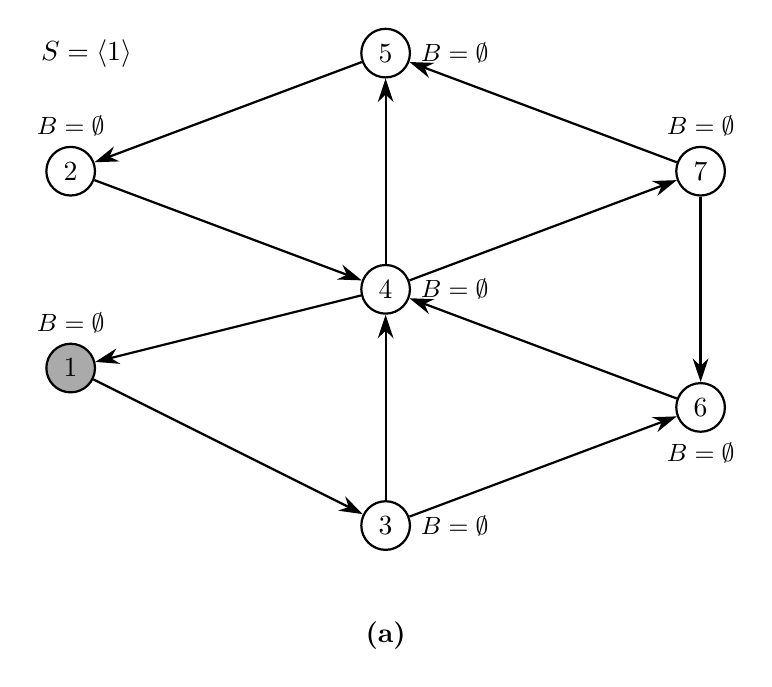
\begin{tikzpicture}
            \node[mynode, fill={rgb:black,1;white,2}, label={[align=center]above:{\small $B = \emptyset$}}](n1) at (0,-1){1};
            \node[mynode, fill=white, label={[align=center]above:{\small $B = \emptyset$}}](n2) at (0,1.5){2};
            \node[mynode, fill=white, label={[align=left]right:{\small $B = \emptyset$}}](n3) at (4,-3){3};
            \node[mynode, fill=white, label={[align=left]right:{\small $B = \emptyset$}}](n4) at (4,0){4};
            \node[mynode, fill=white, label={[align=left]right:{\small $B = \emptyset$}}](n5) at (4,3){5};
            \node[mynode, fill=white, label={[align=center]below:{\small $B = \emptyset$}}](n6) at (8,-1.5){6};
            \node[mynode, fill=white, label={[align=center]above:{\small $B = \emptyset$}}](n7) at (8,1.5){7};

            \draw[myarrow](n1) -- (n3);
            \draw[myarrow](n2) -- (n4);
            \draw[myarrow](n3) -- (n4);
            \draw[myarrow](n3) -- (n6);
            \draw[myarrow](n4) -- (n1);
            \draw[myarrow](n4) -- (n5);
            \draw[myarrow](n4) -- (n7);
            \draw[myarrow](n5) -- (n2);
            \draw[myarrow](n6) -- (n4);
            \draw[myarrow](n7) -- (n5);
            \draw[myarrow](n7) -- (n6);

            \node[align=left, xshift=0.2cm, yshift=3cm] (label2) {$S = \langle 1 \rangle$};
            \node[below=10mm] at (4, -3.1) {\textbf{(a)}};
        \end{tikzpicture}
        \quad \quad \quad
        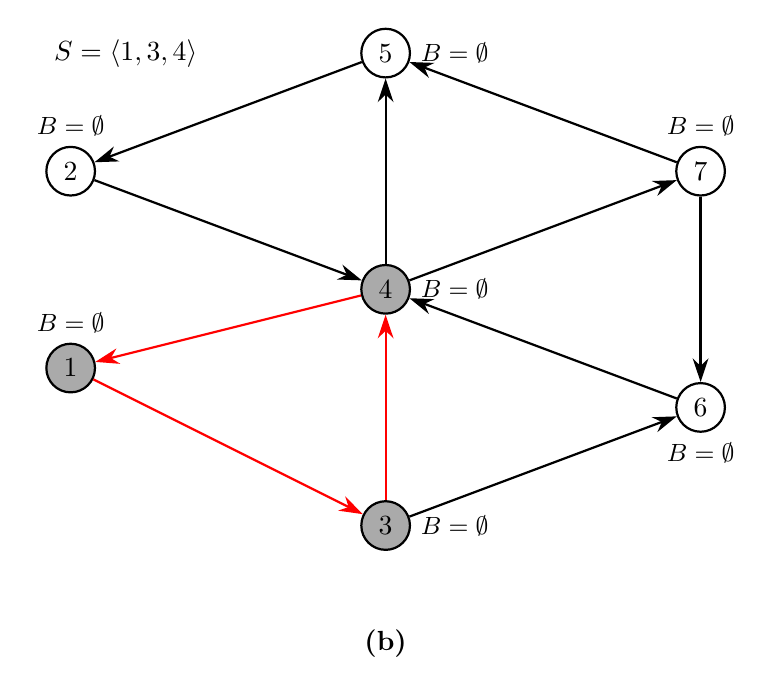
\begin{tikzpicture}

            \node[mynode, fill={rgb:black,1;white,2}, label={[align=center]above:{\small $B = \emptyset$}}](n1) at (0,-1){1};
            \node[mynode, fill=white, label={[align=center]above:{\small $B = \emptyset$}}](n2) at (0,1.5){2};
            \node[mynode, fill={rgb:black,1;white,2}, label={[align=left]right:{\small $B = \emptyset$}}](n3) at (4,-3){3};
            \node[mynode, fill={rgb:black,1;white,2}, label={[align=left]right:{\small $B = \emptyset$}}](n4) at (4,0){4};
            \node[mynode, fill=white, label={[align=left]right:{\small $B = \emptyset$}}](n5) at (4,3){5};
            \node[mynode, fill=white, label={[align=center]below:{\small $B = \emptyset$}}](n6) at (8,-1.5){6};
            \node[mynode, fill=white, label={[align=center]above:{\small $B = \emptyset$}}](n7) at (8,1.5){7};

            \draw[myarrow, color=red](n1) -- (n3);
            \draw[myarrow](n2) -- (n4);
            \draw[myarrow, color=red](n3) -- (n4);
            \draw[myarrow](n3) -- (n6);
            \draw[myarrow, color=red](n4) -- (n1);
            \draw[myarrow](n4) -- (n5);
            \draw[myarrow](n4) -- (n7);
            \draw[myarrow](n5) -- (n2);
            \draw[myarrow](n6) -- (n4);
            \draw[myarrow](n7) -- (n5);
            \draw[myarrow](n7) -- (n6);

            \node[align=left, xshift=0.7cm, yshift=3cm] (label2) {$S = \langle 1, 3, 4 \rangle$};
            \node[below=10mm] at (4, -3.2) {\textbf{(b)}};
        \end{tikzpicture}
    }

    \resizebox{!}{6cm}{
        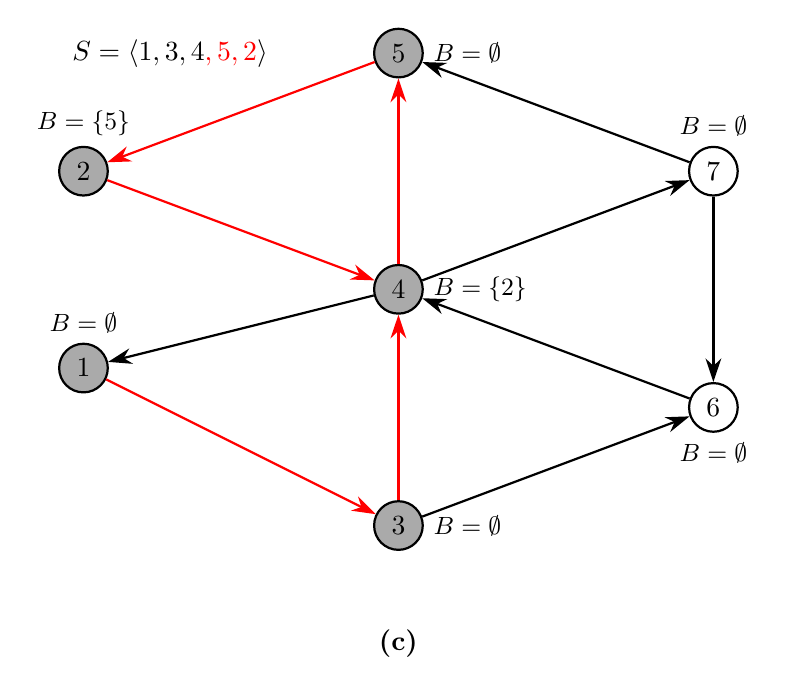
\begin{tikzpicture}
            \node[mynode, fill={rgb:black,1;white,2}, label={[align=center]above:{\small $B = \emptyset$}}](n1) at (0,-1){1};
            \node[mynode, fill={rgb:black,1;white,2}, label={[align=center]above:{\small $B = \{5\}$}}](n2) at (0,1.5){2};
            \node[mynode, fill={rgb:black,1;white,2}, label={[align=left]right:{\small $B = \emptyset$}}](n3) at (4,-3){3};
            \node[mynode, fill={rgb:black,1;white,2}, label={[align=left]right:{\small $B = \{2\}$}}](n4) at (4,0){4};
            \node[mynode, fill={rgb:black,1;white,2}, label={[align=left]right:{\small $B = \emptyset$}}](n5) at (4,3){5};
            \node[mynode, fill=white, label={[align=center]below:{\small $B = \emptyset$}}](n6) at (8,-1.5){6};
            \node[mynode, fill=white, label={[align=center]above:{\small $B = \emptyset$}}](n7) at (8,1.5){7};

            \draw[myarrow, color=red](n1) -- (n3);
            \draw[myarrow, color=red](n2) -- (n4);
            \draw[myarrow, color=red](n3) -- (n4);
            \draw[myarrow](n3) -- (n6);
            \draw[myarrow](n4) -- (n1);
            \draw[myarrow, color=red](n4) -- (n5);
            \draw[myarrow](n4) -- (n7);
            \draw[myarrow, color=red](n5) -- (n2);
            \draw[myarrow](n6) -- (n4);
            \draw[myarrow](n7) -- (n5);
            \draw[myarrow](n7) -- (n6);

            \node[align=left, xshift=1.1cm, yshift=3cm] (label2) {$S = \langle 1, 3, 4 {\color{red}, 5, 2} \rangle$};
            \node[below=10mm] at (4, -3.2) {\textbf{(c)}};
        \end{tikzpicture}
        \quad \quad \quad
        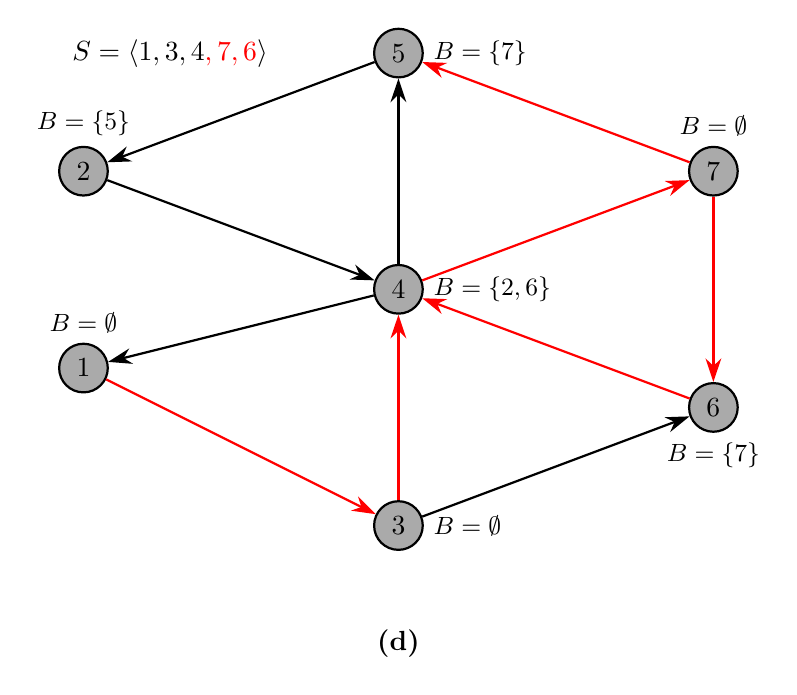
\begin{tikzpicture}
            \node[mynode, fill={rgb:black,1;white,2}, label={[align=center]above:{\small $B = \emptyset$}}](n1) at (0,-1){1};
            \node[mynode, fill={rgb:black,1;white,2}, label={[align=center]above:{\small $B = \{5\}$}}](n2) at (0,1.5){2};
            \node[mynode, fill={rgb:black,1;white,2}, label={[align=left]right:{\small $B = \emptyset$}}](n3) at (4,-3){3};
            \node[mynode, fill={rgb:black,1;white,2}, label={[align=left]right:{\small $B = \{2, 6\}$}}](n4) at (4,0){4};
            \node[mynode, fill={rgb:black,1;white,2}, label={[align=left]right:{\small $B = \{7\}$}}](n5) at (4,3){5};
            \node[mynode, fill={rgb:black,1;white,2}, label={[align=center]below:{\small $B = \{7\}$}}](n6) at (8,-1.5){6};
            \node[mynode, fill={rgb:black,1;white,2}, label={[align=center]above:{\small $B = \emptyset$}}](n7) at (8,1.5){7};

            \draw[myarrow, color=red](n1) -- (n3);
            \draw[myarrow](n2) -- (n4);
            \draw[myarrow, color=red](n3) -- (n4);
            \draw[myarrow](n3) -- (n6);
            \draw[myarrow](n4) -- (n1);
            \draw[myarrow](n4) -- (n5);
            \draw[myarrow, color=red](n4) -- (n7);
            \draw[myarrow](n5) -- (n2);
            \draw[myarrow, color=red](n6) -- (n4);
            \draw[myarrow, color=red](n7) -- (n5);
            \draw[myarrow, color=red](n7) -- (n6);

            \node[align=left, xshift=1.1cm, yshift=3cm] (label2) {$S = \langle 1, 3, 4 {\color{red}, 7, 6} \rangle$};
            \node[below=10mm] at (4, -3.2) {\textbf{(d)}};
        \end{tikzpicture}
    }

\resizebox{!}{6cm}{
    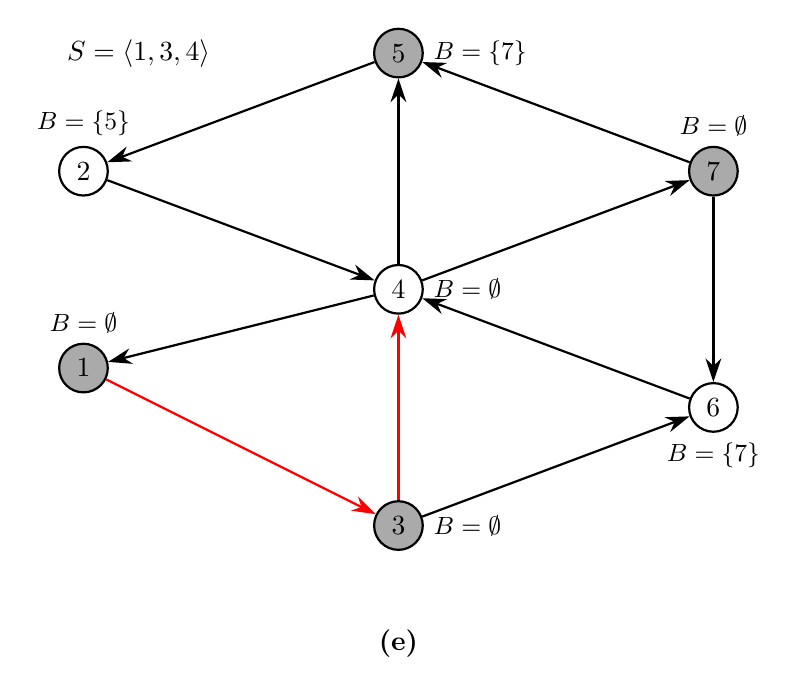
\begin{tikzpicture}
        \node[mynode, fill={rgb:black,1;white,2}, label={[align=center]above:{\small $B = \emptyset$}}](n1) at (0,-1){1};
        \node[mynode, fill=white, label={[align=center]above:{\small $B = \{5\}$}}](n2) at (0,1.5){2};
        \node[mynode, fill={rgb:black,1;white,2}, label={[align=left]right:{\small $B = \emptyset$}}](n3) at (4,-3){3};
        \node[mynode, fill=white, label={[align=left]right:{\small $B = \emptyset$}}](n4) at (4,0){4};
        \node[mynode, fill={rgb:black,1;white,2}, label={[align=left]right:{\small $B = \{7\}$}}](n5) at (4,3){5};
        \node[mynode, fill=white, label={[align=center]below:{\small $B = \{7\}$}}](n6) at (8,-1.5){6};
        \node[mynode, fill={rgb:black,1;white,2}, label={[align=center]above:{\small $B = \emptyset$}}](n7) at (8,1.5){7};

        \draw[myarrow, color=red](n1) -- (n3);
        \draw[myarrow](n2) -- (n4);
        \draw[myarrow, color=red](n3) -- (n4);
        \draw[myarrow](n3) -- (n6);
        \draw[myarrow](n4) -- (n1);
        \draw[myarrow](n4) -- (n5);
        \draw[myarrow](n4) -- (n7);
        \draw[myarrow](n5) -- (n2);
        \draw[myarrow](n6) -- (n4);
        \draw[myarrow](n7) -- (n5);
        \draw[myarrow](n7) -- (n6);

        \node[align=left, xshift=0.7cm, yshift=3cm] (label2) {$S = \langle 1, 3, 4 \rangle$};
        \node[below=10mm] at (4, -3.2) {\textbf{(e)}};
    \end{tikzpicture}
    \quad \quad \quad
    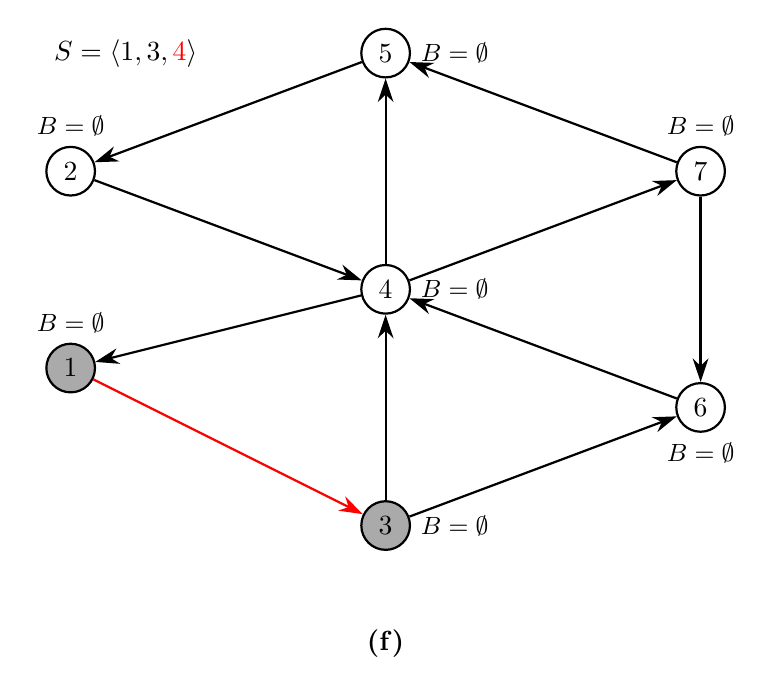
\begin{tikzpicture}
        \node[mynode, fill={rgb:black,1;white,2}, label={[align=center]above:{\small $B = \emptyset$}}](n1) at (0,-1){1};
        \node[mynode, fill=white, label={[align=center]above:{\small $B = \emptyset$}}](n2) at (0,1.5){2};
        \node[mynode, fill={rgb:black,1;white,2}, label={[align=left]right:{\small $B = \emptyset$}}](n3) at (4,-3){3};
        \node[mynode, fill=white, label={[align=left]right:{\small $B = \emptyset$}}](n4) at (4,0){4};
        \node[mynode, fill=white, label={[align=left]right:{\small $B = \emptyset$}}](n5) at (4,3){5};
        \node[mynode, fill=white, label={[align=center]below:{\small $B = \emptyset$}}](n6) at (8,-1.5){6};
        \node[mynode, fill=white, label={[align=center]above:{\small $B = \emptyset$}}](n7) at (8,1.5){7};

        \draw[myarrow, color=red](n1) -- (n3);
        \draw[myarrow](n2) -- (n4);
        \draw[myarrow](n3) -- (n4);
        \draw[myarrow](n3) -- (n6);
        \draw[myarrow](n4) -- (n1);
        \draw[myarrow](n4) -- (n5);
        \draw[myarrow](n4) -- (n7);
        \draw[myarrow](n5) -- (n2);
        \draw[myarrow](n6) -- (n4);
        \draw[myarrow](n7) -- (n5);
        \draw[myarrow](n7) -- (n6);

        \node[align=left, xshift=0.7cm, yshift=3cm] (label2) {$S = \langle 1, 3, {\color{red}4} \rangle$};
        \node[below=10mm] at (4, -3.2) {\textbf{(f)}};
    \end{tikzpicture}
}
\caption{Fasi rilevanti dell'applicazione della procedura CIRCUIT}\label{fig:cicruit-example}
\end{figure}

\newpage

\nlparagraph{Complessit\`a}
Come discusso nella trattazione originale~\cite{doi:10.1137/0204007}, la complessit\`a dell'algoritmo di Johnson
\`e $O((n + m)(c + 1))$, dove $n$ \`e il numero di nodi, $m$ il numero di archi e $c$ il numero di circuiti semplici
presenti nel grafo.
Questo risultato \`e ottenuto considerando che tutti i nodi e gli archi del grafo possono essere visitati al pi\`u una
volta per ogni circuito elementare presente, ovvero che l'algoritmo impiega al pi\`u $O(n + m)$ tempo tra l'output di
un circuito e l'individuazione del successivo.
In particolare, ciascun nodo pu\`o essere bloccato al pi\`u una volta per ogni circuito, e non pu\`o passare pi\`u di
di $O(n + m)$ tempo tra il blocco di un nodo e il suo sblocco. \newline

Si noti tuttavia che, pur essendo l'algoritmo di Johnson pi\`u efficiente rispetto ad altri algoritmi proposti, la
complessit\`a computazionale nel caso peggiore (ovvero quello di un grafo completo) risulta essere maggiore dell'
esponenziale, dovuto al numero di circuiti semplici presenti, che in tal caso \`e pari a

\begin{equation*}
    c \quad = \quad \sum_{i = 1}^{n-1} \binom{n}{n-i+1} (n-1)!
\end{equation*}



\section{Contrazione di Grafi}\label{sec:contrazione-di-grafi}

Nella teoria dei grafi la contrazione di un grafo \`e un'operazione che permette di ridurre la dimensione di un grafo
senza alterarne la struttura fondamentale. \newline
La contrazione di archi o di sottoinsiemi di nodi \`e un operazione fondamentale nella teoria dei grafi minori, dove
si studiano le propriet\`a di un grafo in relazione alla presenza di sottostrutture minori ottenibili attraverso
rimozione di archi e nodi o contrazioni. \newline
Queste tecniche di contrazione trovano applicazione in tutti quei casi in cui si vuole semplificare un grafo
identificando i vertici che possono essere considerati equivalenti in relazione ad una certa propriet\`a,
e risultano essere utili in svariati problemi di ottimizzazione e partizionamento di grafi.
In letteratura, le operazioni di contrazione di grafi sono state utilizzate anche a scopo di compressione di grafi,
al fine di renderli pi\`u compatti e trattabili con algoritmi di analisi altrimenti troppo costosi,
individuando schemi di contrazione d'interesse e cercando di evitare perdita di
informazione~\cite{10.1145/3448016.3452797}. \newline


\subsection{Contrazione di archi}\label{subsec:contrazione-di-archi}

La contrazione di archi, spesso riferita come contrazione di spigoli, di un grafo orientato $G = (V, E)$ \`e
un'operazione che consiste nella rimozione di un  arco $e = (u, v) \in E$ e nella simultanea fusione dei nodi $u$ e
$v$ in un unico nodo $w$.
Quando ci\`o avviene, tutti gli archi che entrano in $u$ e $v$ diventano archi entranti in $w$, e, analogamente,
tutti gli archi che escono da $u$ e $v$ diventano archi uscenti da $w$.
Il risultato di una tale operazione \`e, quindi, un nuovo grafo ottenuto da $G$ mediante la contrazione
dell'arco $e$, che pu\`o essere indicato con $G/e$ (da non confondersi con la sottrazione insiemistica $\setminus$).
Si noti che, secondo la definzione data, una tale operazione applicata ad un grafo orientato semplice pu\`o risultare
in un grafo con archi multipli e cappi, a seconda della struttura del grafo iniziale.
Per questo \`e spesso previsto nella definzione di contrazione di archi che vengano applicate le ulteriori operazioni
necessarie ad ottenere come risultato un nuovo grafo semplice.

\begin{definition}[Contrazione di archi]
Sia $G = (V, E)$ un grafo orientato e sia $e = (u, v) \in E$ un arco di $G$ con $u \neq v$,
sia $f$ una funzione su $V$ che associa ogni nodo in $V \setminus \{u, v\}$ a se stesso, o ad un nuovo nodo $w$
altrimenti. \newline
La contrazione di $e$ su $G$ \`e un nuovo grafo $G' = (V', E')$ dove:
\begin{itemize}
    \item $V' = (V \setminus \{u, v\}) \cup \{w\}$ con $w \notin V$
    \item $E' = \{(f(x), f(y)) \mid (x, y) \in E \setminus \{e\}\}$
\end{itemize}
\end{definition}

\begin{figure}[h]
    \centering
    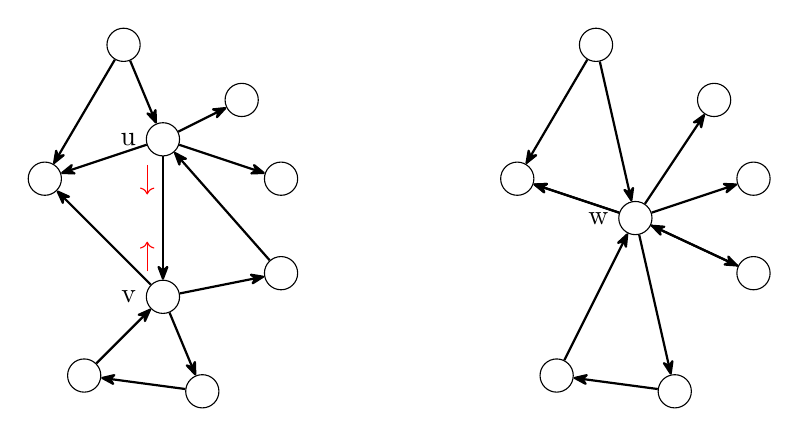
\begin{tikzpicture}
  % Styles for the nodes and edges
  \tikzstyle{vertex} = [draw, circle, inner sep=2pt, minimum size=12pt]
  \tikzstyle{edge} = [->, >={Stealth[round]}, thick]

  % Left Graph
  \node[vertex, label=left:u] (u) at (0, 1) {};
  \node[] (u2) at (-0.2, 0.8) {};
  \node[vertex, label=left:v] (v) at (0, -1) {};
  \node[] (v2) at (-0.2, -0.8) {};

  \node[vertex] (a) at (-1.5, 0.5) {};
  \node[vertex] (b) at (1.5, 0.5) {};
  \node[vertex] (c) at (-0.5, 2.2) {};
  \node[vertex] (d) at (1, 1.5) {};
  \node[vertex] (e) at (-1, -2) {};
  \node[vertex] (f) at (1.5, -0.7) {};
  \node[vertex] (g) at (0.5, -2.2) {};

  \draw[edge] (u) -- (a);
  \draw[edge] (u) -- (b);
  \draw[edge] (c) -- (u);
  \draw[edge] (u) -- (d);
  \draw[edge] (f) -- (u);
  \draw[edge] (c) -- (a);

  \draw[edge] (v) -- (a);
  \draw[edge] (e) -- (v);
  \draw[edge] (v) -- (f);
  \draw[edge] (v) -- (g);
  \draw[edge] (g) -- (e);

  \draw[edge] (u) -- (v);
  \draw[->, red] (u2) -- ++( 0, -0.5);
  \draw[->, red] (v2) -- ++( 0, 0.5);

  % Right Graph
  \node[vertex, label=left:w] (w) at (6, 0) {};

  \node[vertex] (a2) at (4.5, 0.5) {};
  \node[vertex] (b2) at (7.5, 0.5) {};
  \node[vertex] (c2) at (5.5, 2.2) {};
  \node[vertex] (d2) at (7, 1.5) {};
  \node[vertex] (e2) at (5, -2) {};
  \node[vertex] (f2) at (7.5, -0.7) {};
  \node[vertex] (g2) at (6.5, -2.2) {};

  \draw[edge] (w) -- (a2);
  \draw[edge] (w) -- (b2);
  \draw[edge] (c2) -- (w);
  \draw[edge] (w) -- (d2);
  \draw[edge] (f2) -- (w);
  \draw[edge] (c2) -- (a2);

  \draw[edge] (w) -- (a2);
  \draw[edge] (e2) -- (w);
  \draw[edge] (w) -- (f2);
  \draw[edge] (w) -- (g2);
  \draw[edge] (g2) -- (e2);

\end{tikzpicture}
    \caption{Esempio di contrazione di un arco in un grafo orientato}
    \label{fig:edge-contraction-example}
\end{figure}

In figura~\ref{fig:edge-contraction-example} \`e mostrato un esempio di contrazione di un arco $(u, v)$ in un nuovo
nodo $w$ in un grafo orientato, che include la rimozione di archi multipli e di cappi.
Pi\`u in generale, una tale operazione pu\`o essere eeguita su un insieme di archi, contraendo ciacuno di essi in
un qualsiasi ordine.

\subsection{Contrazione di sottografi}\label{subsec:contrazione-di-sottografi}
Un'operazione simile alla contrazione di archi, ma pi\`u generale, \`e la \textbf{contrazione di vertici}
(o \textbf{identificazione di vertici}) di un grafo.
Essa pu\`o essere vista come una generalizzazione della contrazione di archi, in quanto rimuove la restrizione che
la coppia di nodi da contrarre sia adiacente, rendendo la contrazione per archi un suo caso particolare.
Si immagini, pertanto, di avere il grafo a sinistra della figura~\ref{fig:subgraph-contraction-example} privato,
per\`o, dell'arco $(u, v)$.
La contrazione per vertici permetterebbe di contrarre la coppia non adiacente di nodi $u$ e $v$, risultando,
comunque, nel grafo a destra della figura~\ref{fig:subgraph-contraction-example}. \newline

L' operazione di contrazione di vertici pu\`o essere generalizzata nella \textbf{contrazione di sottografi},
un'operazione che permette di contrarre un qualsiasi sottoinsieme di nodi di un grafo in un unico nodo.
Dato un grafo $G = (E_G, V_G)$ ed un suo sottografo $H = (V_H, E_H)$, quindi, il grafo risultante dalla contrazione
di $H$ mantiene tutti gli archi incidenti su coppie di nodi in $E_G \setminus E_H$, sostituendo
quegli archi incidenti tra nodi in $V_G \setminus V_H$ e $V_H$ con nuovi archi incidenti sul nuovo nodo contratto.

\begin{definition}[Contrazione di sottografi]
    Sia $G = (V, E)$ un grafo orientato, sia $W \subseteq V$ un sottoinsieme di nodi di $G$, sia $H = G[W] = (W, F)$
    il sottografo indotto da $W$ in $G$.
    Sia $f$ una funzione su $V$ che associa ogni nodo in $V \setminus W$ a se stesso, o ad un nuovo nodo $w$
    altrimenti.
    La contrazione di $H$ su $G$ \`e un nuovo grafo $G' = (V', E')$ dove:
    \begin{itemize}
        \item $V' = (V \setminus W) \cup \{w\}$ con $w \notin V$
        \item $E' = \{(f(u), f(v)) \mid (u, v) \in E \setminus F\}$
    \end{itemize}
\end{definition}

\begin{figure}[h]
    \centering
    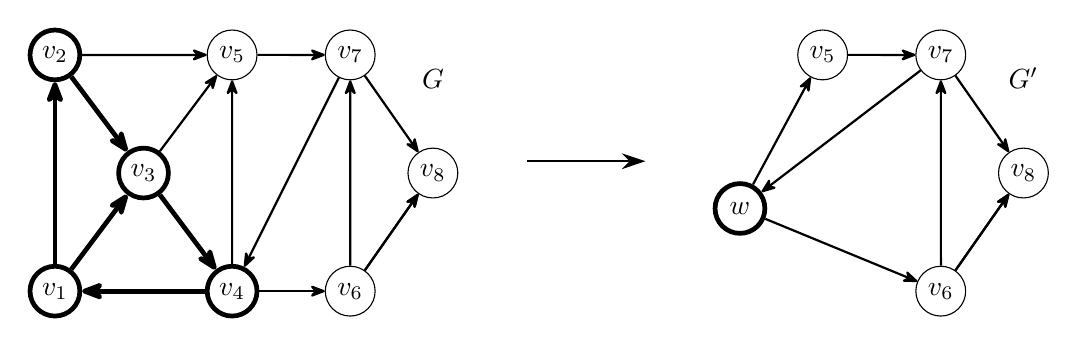
\begin{tikzpicture}[scale=1.5]

% Define the styles for the nodes and edges
\tikzstyle{vertex} = [draw, circle, inner sep=2pt, minimum size=18pt]
\tikzstyle{edge} = [->, >={Stealth[round]}, thick]
\tikzset{thick vertex/.style = {draw, circle, inner sep=2pt, minimum size=18pt, line width=1.7pt}}]
\tikzset{thick edge/.style = {->, >={Stealth[round]}, line width=1.7pt}}

% Left graph
\node[] (g) at (3.2,1.8) {$G$};

\node[thick vertex] (v1) at (0,0) {$v_1$};
\node[thick vertex] (v2) at (0,2) {$v_2$};
\node[thick vertex] (v3) at (0.75,1) {$v_3$};
\node[thick vertex] (v4) at (1.5,0) {$v_4$};
\node[vertex] (v5) at (1.5,2) {$v_5$};
\node[vertex] (v6) at (2.5,0) {$v_6$};
\node[vertex] (v7) at (2.5,2) {$v_7$};
\node[vertex] (v8) at (3.2,1) {$v_8$};

% Draw edges for left graph
\draw[thick edge] (v1) -- (v2);
\draw[thick edge] (v1) -- (v3);
\draw[thick edge] (v2) -- (v3);
\draw[thick edge] (v3) -- (v4);
\draw[thick edge] (v4) -- (v1);
\draw[edge] (v2) -- (v5);
\draw[edge] (v3) -- (v5);
\draw[edge] (v4) -- (v5);
\draw[edge] (v4) -- (v6);
\draw[edge] (v5) -- (v7);
\draw[edge] (v6) -- (v7);
\draw[edge] (v6) -- (v8);
\draw[edge] (v7) -- (v4);
\draw[edge] (v7) -- (v8);
\draw[edge] (v6) -- (v8);

% Right graph
\node[] (g2) at (8.2,1.8) {$G'$};

\node[thick vertex] (w) at (5.8,0.7) {$w$};
\node[vertex] (v5) at (6.5,2) {$v_5$};
\node[vertex] (v6) at (7.5,0) {$v_6$};
\node[vertex] (v7) at (7.5,2) {$v_7$};
\node[vertex] (v8) at (8.2,1) {$v_8$};

% Draw edges for right graph
\draw[edge] (w) -- (v5);
\draw[edge] (w) -- (v6);
\draw[edge] (v5) -- (v7);
\draw[edge] (v6) -- (v7);
\draw[edge] (v6) -- (v8);
\draw[edge] (v7) -- (w);
\draw[edge] (v7) -- (v8);
\draw[edge] (v6) -- (v8);

% Draw the arrow
\draw[-{Stealth[length=3mm, width=2mm]}, thick] (4,1.1) -- (5,1.1);

\end{tikzpicture}
    \caption{Esempio di contrazione di un sottografo in un grafo orientato}
    \label{fig:subgraph-contraction-example}
\end{figure}

In figura~\ref{fig:subgraph-contraction-example} \`e mostrato un esempio di contrazione di un sottografo
$G[\{v_1, v_2, v_3, v_4\}]$ del grafo orientato $G$ in un nuovo nodo $w$, che include la rimozione di archi multipli
e di cappi. \newline

Alla luce delle definizioni delle operazioni presentate, valgono le seguenti considerazioni:
\begin{itemize}
    \item Il risultato della contrazione di una coppia di nodi adiacienti su un certo grafo $G$ pu\`o produrre un
    grafo isomorfo a quello della contrazione di una coppia di nodi non adiacenti in un altro grafo $G'$ non isomorfo
    a $G$.
    \`E il caso precedentemente considerato applicato al grafo a sinistra in figura~\ref{fig:edge-contraction-example}.
    \item Il risultato della contrazione di un sottografo su un certo grafo $G$ pu\`o produrre un grafo isomorfo
    a quello della contrazione di un sottografo in un altro grafo $G'$ non isomorfo a $G$.
    Come esempio analogo, basta considerare un grafo $J$ ottenuto a apartire dal grafo $G$ in
    figura~\ref{fig:subgraph-contraction-example} rimuovendo il nodo $v_1$ e i suoi archi incidenti.
    I grafi risultanti dalla contrazione di $G[\{v_1, v_2, v_3, v_4\}]$ in $G$ e dalla contrazione di
    $J[\{v_2, v_3, v_4\}]$ in $G'$ saranno certamente isomorfi.
\end{itemize}

Questo significa che la contrazione di vertici e di sottografi non sono operazioni invertibili, in quanto
rappresentano funzioni suriettive ma non iniettive.
Di fatti queste operazioni non mantengono alcuna informazione legata alla struttura originale del grafo su cui
sono applicate.
Come mostrato nel capitolo~\ref{cap:grafi-multi-livello}, tra gli obiettivi della definizione del grafo multi-livello,
vi \`e proprio quello di mantenere le informazioni legate alla struttura dei grafi a cui sono applicate contrazioni,
permettendo anche operazioni di decontrazione.

\subsection{Grafi quoziente}\label{subsec:grafi-quoziente}

Nella teoria dei grafi, un grafo quoziente \`e una visione astratta di un grafo partizionato in sottoinsiemi di nodi
che rappresenta le relazioni tra tali sottoinsiemi.
In un grafo quoziente $G'$ ottenuto a partire da un grafo $G = (V, E)$, i nodi rappresentano ``blocchi'' di nodi di $G$
che fanno parte dello stesso insieme per una qualche partizione di $V$.
Per quanto riguarda gli archi di $G'$, dati due blocchi di nodi $B_1$ e $B_2$ in $G'$, un arco tra $B_1$ e $B_2$ sta
ad indicare la presenza di almeno un arco tra un nodo di $B_1$ e un nodo di $B_2$ in $G$.

Se intuitivamente si potrebbe dire che il grafo quoziente permette di accorpare gruppi di nodi e archi tra loro
per formare un nuovo grafo, una descrizione pi\`u formale utilizzerebbe il concetto di contrazione di sottografi,
definendo il grafo quoziente come il risultato delle contrazioni dei sottografi indotti dalla data partizione di nodi.

\begin{definition}[Grafo Quoziente]
Sia $G = (V, E)$ un grafo orientato, sia $P \subseteq \mathcal{P}(V)$ una partizione di $V$, sia $R$ la relazione
d'equivalenza su $V$ indotta dalla partizione $P$.
Il grafo quoziente di $G$ rispetto a $P$ \`e il grafo $G' = (V', E')$ dove:
    \begin{itemize}
        \item $V'$ \`e l'insieme quoziente $V/R$, ovvero l'insieme delle classi di equivalenza di $R$ su $V$.
        \item $E' = \{([u]_R, [v]_R) \mid (u, v) \in E\}$, dove $[u]_R$ e $[v]_R$ sono rispettivamente le classi di
        equivalenza dei nodi $u$ e $v$ rispetto a $R$.
    \end{itemize}
\end{definition}

\begin{figure}[h]
    \centering
    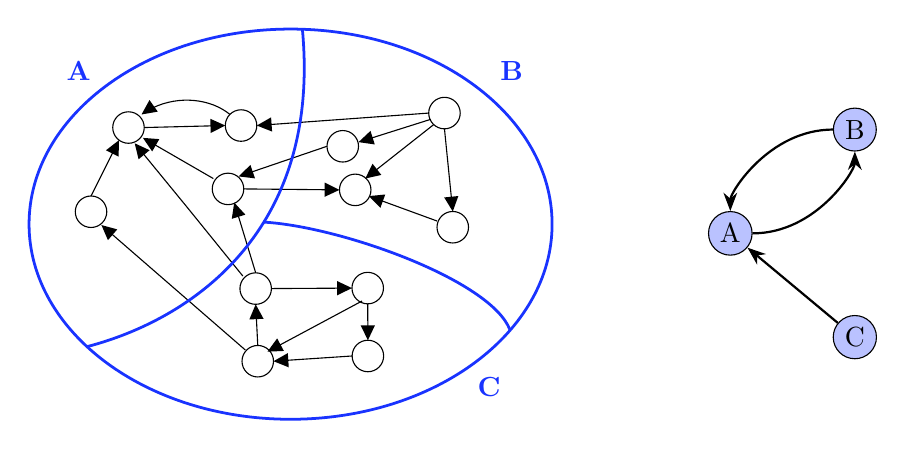
\begin{tikzpicture}[x=0.75pt,y=0.75pt,yscale=-1,xscale=1,graph node/.style={circle, draw, inner sep=2pt}, >={Stealth}]
%uncomment if require: \path (0,193); %set diagram left start at 0, and has height of 193

%Shape: Ellipse [id:dp5716078870574002]
\draw   (157.72,126.37) .. controls (157.72,122.18) and (161.11,118.78) .. (165.3,118.78) .. controls (169.49,118.78) and (172.89,122.18) .. (172.89,126.37) .. controls (172.89,130.56) and (169.49,133.96) .. (165.3,133.96) .. controls (161.11,133.96) and (157.72,130.56) .. (157.72,126.37) -- cycle ;
%Straight Lines [id:da030036293703488592]
\draw    (162.59,132.58) -- (119.64,155.58) ;
\draw [shift={(117,157)}, rotate = 331.82] [fill={rgb, 255:red, 0; green, 0; blue, 0 }  ][line width=0.08]  [draw opacity=0] (7.14,-3.43) -- (0,0) -- (7.14,3.43) -- cycle    ;
%Shape: Ellipse [id:dp4694008742489806]
\draw   (96.69,48.05) .. controls (96.69,43.86) and (100.09,40.46) .. (104.28,40.46) .. controls (108.47,40.46) and (111.87,43.86) .. (111.87,48.05) .. controls (111.87,52.24) and (108.47,55.64) .. (104.28,55.64) .. controls (100.09,55.64) and (96.69,52.24) .. (96.69,48.05) -- cycle ;
%Shape: Ellipse [id:dp43075157044098433]
\draw   (157.8,159.08) .. controls (157.8,154.89) and (161.2,151.49) .. (165.39,151.49) .. controls (169.58,151.49) and (172.98,154.89) .. (172.98,159.08) .. controls (172.98,163.27) and (169.58,166.67) .. (165.39,166.67) .. controls (161.2,166.67) and (157.8,163.27) .. (157.8,159.08) -- cycle ;
%Straight Lines [id:da7735175864839863]
\draw    (157.8,159.08) -- (122.91,161.4) ;
\draw [shift={(119.91,161.6)}, rotate = 356.19] [fill={rgb, 255:red, 0; green, 0; blue, 0 }  ][line width=0.08]  [draw opacity=0] (7.14,-3.43) -- (0,0) -- (7.14,3.43) -- cycle    ;
%Shape: Ellipse [id:dp8331515179192863]
\draw   (103.74,126.6) .. controls (103.74,122.41) and (107.14,119.01) .. (111.33,119.01) .. controls (115.52,119.01) and (118.91,122.41) .. (118.91,126.6) .. controls (118.91,130.79) and (115.52,134.19) .. (111.33,134.19) .. controls (107.14,134.19) and (103.74,130.79) .. (103.74,126.6) -- cycle ;
%Straight Lines [id:da8805781538281761]
\draw    (165.3,133.96) -- (165.38,148.49) ;
\draw [shift={(165.39,151.49)}, rotate = 269.72] [fill={rgb, 255:red, 0; green, 0; blue, 0 }  ][line width=0.08]  [draw opacity=0] (7.14,-3.43) -- (0,0) -- (7.14,3.43) -- cycle    ;
%Shape: Ellipse [id:dp11540879760206746]
\draw   (24.41,89.59) .. controls (24.41,85.4) and (27.81,82) .. (32,82) .. controls (36.19,82) and (39.59,85.4) .. (39.59,89.59) .. controls (39.59,93.78) and (36.19,97.17) .. (32,97.17) .. controls (27.81,97.17) and (24.41,93.78) .. (24.41,89.59) -- cycle ;
%Straight Lines [id:da7303103534852602]
\draw    (90.93,73.6) -- (90.93,73.6) -- (59.6,55.5) ;
\draw [shift={(57,54)}, rotate = 30.02] [fill={rgb, 255:red, 0; green, 0; blue, 0 }  ][line width=0.08]  [draw opacity=0] (7.14,-3.43) -- (0,0) -- (7.14,3.43) -- cycle    ;
%Shape: Ellipse [id:dp18097418973582324]
\draw   (42.46,49.02) .. controls (42.46,44.83) and (45.85,41.43) .. (50.04,41.43) .. controls (54.23,41.43) and (57.63,44.83) .. (57.63,49.02) .. controls (57.63,53.21) and (54.23,56.6) .. (50.04,56.6) .. controls (45.85,56.6) and (42.46,53.21) .. (42.46,49.02) -- cycle ;
%Straight Lines [id:da4155132765855869]
\draw    (57.63,49.02) -- (93.69,48.12) ;
\draw [shift={(96.69,48.05)}, rotate = 178.58] [fill={rgb, 255:red, 0; green, 0; blue, 0 }  ][line width=0.08]  [draw opacity=0] (7.14,-3.43) -- (0,0) -- (7.14,3.43) -- cycle    ;
%Straight Lines [id:da1262374391562433]
\draw    (32,82) -- (44.09,57.83) ;
\draw [shift={(45.43,55.14)}, rotate = 116.57] [fill={rgb, 255:red, 0; green, 0; blue, 0 }  ][line width=0.08]  [draw opacity=0] (7.14,-3.43) -- (0,0) -- (7.14,3.43) -- cycle    ;
%Straight Lines [id:da572291236631852]
\draw    (105.14,120.57) -- (78.69,87.9) -- (54.94,58.92) ;
\draw [shift={(53.04,56.6)}, rotate = 50.66] [fill={rgb, 255:red, 0; green, 0; blue, 0 }  ][line width=0.08]  [draw opacity=0] (7.14,-3.43) -- (0,0) -- (7.14,3.43) -- cycle    ;
%Curve Lines [id:da021365012814849704]
\draw    (98.95,42.72) .. controls (89.68,35.14) and (74.55,33.42) .. (61.85,39.48) .. controls (60.82,39.97) and (59.81,40.51) .. (58.82,41.1) ;
\draw [shift={(56.34,42.72)}, rotate = 324.46] [fill={rgb, 255:red, 0; green, 0; blue, 0 }  ][line width=0.08]  [draw opacity=0] (7.14,-3.43) -- (0,0) -- (7.14,3.43) -- cycle    ;
%Shape: Ellipse [id:dp776996888716095]
\draw   (90.41,78.59) .. controls (90.41,74.4) and (93.81,71) .. (98,71) .. controls (102.19,71) and (105.59,74.4) .. (105.59,78.59) .. controls (105.59,82.78) and (102.19,86.17) .. (98,86.17) .. controls (93.81,86.17) and (90.41,82.78) .. (90.41,78.59) -- cycle ;
%Shape: Ellipse [id:dp46756955428949243]
\draw   (104.74,161.6) .. controls (104.74,157.41) and (108.14,154.01) .. (112.33,154.01) .. controls (116.52,154.01) and (119.91,157.41) .. (119.91,161.6) .. controls (119.91,165.79) and (116.52,169.19) .. (112.33,169.19) .. controls (108.14,169.19) and (104.74,165.79) .. (104.74,161.6) -- cycle ;
%Straight Lines [id:da11987408246874143]
\draw    (112.33,154.01) -- (111.48,137.18) ;
\draw [shift={(111.33,134.19)}, rotate = 87.11] [fill={rgb, 255:red, 0; green, 0; blue, 0 }  ][line width=0.08]  [draw opacity=0] (7.14,-3.43) -- (0,0) -- (7.14,3.43) -- cycle    ;
%Straight Lines [id:da7165440164643189]
\draw    (118.91,126.6) -- (154.72,126.39) ;
\draw [shift={(157.72,126.37)}, rotate = 179.66] [fill={rgb, 255:red, 0; green, 0; blue, 0 }  ][line width=0.08]  [draw opacity=0] (7.14,-3.43) -- (0,0) -- (7.14,3.43) -- cycle    ;
%Straight Lines [id:da8702436048031414]
\draw    (106.33,156.19) -- (39.27,97.97) ;
\draw [shift={(37,96)}, rotate = 40.96] [fill={rgb, 255:red, 0; green, 0; blue, 0 }  ][line width=0.08]  [draw opacity=0] (7.14,-3.43) -- (0,0) -- (7.14,3.43) -- cycle    ;
%Straight Lines [id:da01851647212321983]
\draw    (111.33,119.01) -- (101.88,88.04) ;
\draw [shift={(101,85.17)}, rotate = 73.03] [fill={rgb, 255:red, 0; green, 0; blue, 0 }  ][line width=0.08]  [draw opacity=0] (7.14,-3.43) -- (0,0) -- (7.14,3.43) -- cycle    ;
%Shape: Ellipse [id:dp5733943324242119]
\draw   (194.69,42.05) .. controls (194.69,37.86) and (198.09,34.46) .. (202.28,34.46) .. controls (206.47,34.46) and (209.87,37.86) .. (209.87,42.05) .. controls (209.87,46.24) and (206.47,49.64) .. (202.28,49.64) .. controls (198.09,49.64) and (194.69,46.24) .. (194.69,42.05) -- cycle ;
%Shape: Ellipse [id:dp4982173340393281]
\draw   (198.69,97.05) .. controls (198.69,92.86) and (202.09,89.46) .. (206.28,89.46) .. controls (210.47,89.46) and (213.87,92.86) .. (213.87,97.05) .. controls (213.87,101.24) and (210.47,104.64) .. (206.28,104.64) .. controls (202.09,104.64) and (198.69,101.24) .. (198.69,97.05) -- cycle ;
%Shape: Ellipse [id:dp6443249330347911]
\draw   (145.69,58.05) .. controls (145.69,53.86) and (149.09,50.46) .. (153.28,50.46) .. controls (157.47,50.46) and (160.87,53.86) .. (160.87,58.05) .. controls (160.87,62.24) and (157.47,65.64) .. (153.28,65.64) .. controls (149.09,65.64) and (145.69,62.24) .. (145.69,58.05) -- cycle ;
%Shape: Ellipse [id:dp2962874847585506]
\draw   (151.69,79.05) .. controls (151.69,74.86) and (155.09,71.46) .. (159.28,71.46) .. controls (163.47,71.46) and (166.87,74.86) .. (166.87,79.05) .. controls (166.87,83.24) and (163.47,86.64) .. (159.28,86.64) .. controls (155.09,86.64) and (151.69,83.24) .. (151.69,79.05) -- cycle ;
%Straight Lines [id:da08505254887451863]
\draw    (198.69,94.05) -- (168.68,83.08) ;
\draw [shift={(165.87,82.05)}, rotate = 20.08] [fill={rgb, 255:red, 0; green, 0; blue, 0 }  ][line width=0.08]  [draw opacity=0] (7.14,-3.43) -- (0,0) -- (7.14,3.43) -- cycle    ;
%Straight Lines [id:da8488856387468098]
\draw    (105.59,78.59) -- (148.69,79.02) ;
\draw [shift={(151.69,79.05)}, rotate = 180.57] [fill={rgb, 255:red, 0; green, 0; blue, 0 }  ][line width=0.08]  [draw opacity=0] (7.14,-3.43) -- (0,0) -- (7.14,3.43) -- cycle    ;
%Straight Lines [id:da9679144897377887]
\draw    (145.69,58.05) -- (105.98,71.6) ;
\draw [shift={(103.14,72.57)}, rotate = 341.16] [fill={rgb, 255:red, 0; green, 0; blue, 0 }  ][line width=0.08]  [draw opacity=0] (7.14,-3.43) -- (0,0) -- (7.14,3.43) -- cycle    ;
%Straight Lines [id:da895747160462798]
\draw    (194.69,42.05) -- (114.86,47.83) ;
\draw [shift={(111.87,48.05)}, rotate = 355.86] [fill={rgb, 255:red, 0; green, 0; blue, 0 }  ][line width=0.08]  [draw opacity=0] (7.14,-3.43) -- (0,0) -- (7.14,3.43) -- cycle    ;
%Straight Lines [id:da9678052539321507]
\draw    (195.69,45.05) -- (163.73,55.15) ;
\draw [shift={(160.87,56.05)}, rotate = 342.47] [fill={rgb, 255:red, 0; green, 0; blue, 0 }  ][line width=0.08]  [draw opacity=0] (7.14,-3.43) -- (0,0) -- (7.14,3.43) -- cycle    ;
%Straight Lines [id:da12597861271491162]
\draw    (202.28,49.64) -- (205.98,86.48) ;
\draw [shift={(206.28,89.46)}, rotate = 264.26] [fill={rgb, 255:red, 0; green, 0; blue, 0 }  ][line width=0.08]  [draw opacity=0] (7.14,-3.43) -- (0,0) -- (7.14,3.43) -- cycle    ;
%Straight Lines [id:da05573449739087133]
\draw    (197.14,47.57) -- (166.5,71.71) ;
\draw [shift={(164.14,73.57)}, rotate = 321.77] [fill={rgb, 255:red, 0; green, 0; blue, 0 }  ][line width=0.08]  [draw opacity=0] (7.14,-3.43) -- (0,0) -- (7.14,3.43) -- cycle    ;
%Shape: Ellipse [id:dp18633067687908644]
\draw  [color=blue  ,draw opacity=1 ][line width=1]  (2.14,95.57) .. controls (2.14,43.66) and (58.55,1.57) .. (128.14,1.57) .. controls (197.73,1.57) and (254.14,43.66) .. (254.14,95.57) .. controls (254.14,147.49) and (197.73,189.57) .. (128.14,189.57) .. controls (58.55,189.57) and (2.14,147.49) .. (2.14,95.57) -- cycle ;
%Curve Lines [id:da9916896653167908]
\draw [color=blue  ,draw opacity=1 ][line width=1]    (30.14,154.57) .. controls (79.86,141.57) and (142.86,99.57) .. (133.86,2) ;
%Curve Lines [id:da16207253703394464]
\draw [color=blue  ,draw opacity=1 ][line width=1]    (233.86,146.57) .. controls (224.86,122.57) and (151.86,96.57) .. (115,94.57) ;

% Text Node
\draw (19,16) node [anchor=north west][inner sep=0.75pt]    {$\textcolor{blue}{\mathbf{A}}$};
% Text Node
\draw (228,16) node [anchor=north west][inner sep=0.75pt]    {$\textcolor{blue}{\mathbf{B}}$};
% Text Node
\draw (217,168.4) node [anchor=north west][inner sep=0.75pt]    {$\textcolor{blue}{\mathbf{C}}$};


% Define nodes in the condensed graph
\node[graph node, fill=blue!30, draw=black] (A) at (340,100) {A};
\node[graph node, fill=blue!30, draw=black] (B) at (400,50) {B};
\node[graph node, fill=blue!30, draw=black] (C) at (400,150) {C};

% Draw edges in the quotient graph
\draw[->, thick] (A) to[out=0, in=90] (B);
\draw[->, thick] (B) to[out=180, in=270] (A);
\draw[->, thick] (C) -- (A);

\end{tikzpicture}
    \caption{Esempio di grafo quoziente di un grafo orientato}
    \label{fig:quotient-graph-example}
\end{figure}

La figura~\ref{fig:quotient-graph-example} mostra un esempio di grafo quoziente sulla destra ottenuto a partire dal
grafo orientato sulla sinistra e una partizione $P = \{A, B, C\}$. \newline

Come evidente dalla definzione, il nome del grafo quoziente \`e dovuto al fatto che la sua struttura \`e
strettamente legata all'insieme quoziente di una qualche relazione di equivalenza definita sui nodi del grafo.
Sebbene, assieme al grafo di partenza, l'ingrediente fondamentale per la definizione di un grafo quoziente sia la
una partizione dei suoi nodi, una relazione di equivalenza sugli stessi sarebbe un parametro equivalente, in quanto
ogni relazione di equivalenza induce una partizione degli elementi del suo dominio in classi di equivalenza.

Le relazioni di equivalenza, così come le partizioni, possono essere comparate tra
loro secondo il concetto di raffinamento: una relazione di equivalenza $R_1$ si dice più \textbf{fine}
(in inglese \textit{finer}) di un'altra relazione di equivalenza $R_2$ se ogni classe di equivalenza di $R_1$ \`e
contenuta in una classe di equivalenza di $R_2$.
In tal caso si dice che $R_2$ \`e più \textbf{grezza} (in inglese \textit{coarser}) di $R_1$, in quanto ogni classe
di equivalenza di $R_2$ pu\`o essere ottenuta come l'unione di classi di equivalenza di $R_1$. \newline

Per questo \`e interessante notare che tale concetto di finezza pu\`o essere facilmente esteso ai grafi quoziente:
\begin{itemize}
    \item Ogni grafo pu\`o banalmente considerarsi come il grafo quoziente di se stesso rispetto
    alla relazione di equivalenza di ugualianza, in quanto ogni nodo di un grafo \`e uguale unicamente a se stesso.
    La relazione di equivalenza di ugualianza, infatti, \`e la relazione di equivalenza pi\`u fine, e per questo
    genera il grafo quoziente pi\`u fine possibile a partire da qualunque grafo.
    \item Analogamente, il grafo composto di un unico nodo e nessun arco risulta il grafo quoziente di ogni grafo
    rispetto alla relazione di equivalenza universale, che mette in relazione qualsiasi coppia di elementi ed
    identifica tutti i nodi di qualunque grafo in un unico blocco.
    La relazione di equivalenza universale, infatti, \`e la relazione di equivalenza pi\`u grezza e, come \`e
    intuibile pensare, genera il grafo quoziente pi\`u grezzo possibile a partire da qualunque grafo.
\end{itemize}

Una particolare relazione di equivalenza che ben si presta alla definizione di un grafo quoziente \`e la relazione di
mutua raggiungibilit\`a tra nodi di un grafo, che ne definisce le componenti fortemente connesse.
Il grafo quoziente di un grafo rispetto a tale relazione di equivalenza prende il nome di
\textbf{condensazione} (o grafo delle componenti fortemente connesse), e si dimostra essere un grafo diretto aciclico.

\begin{figure}[h]
    \centering
    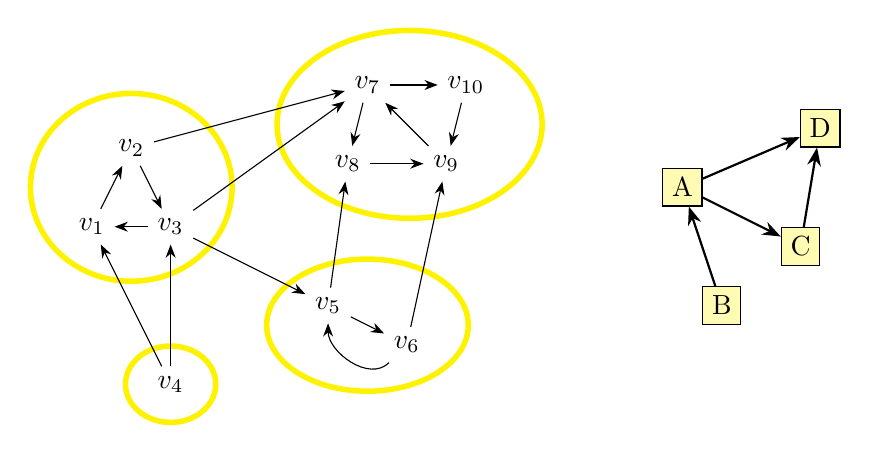
\begin{tikzpicture}[>={Stealth}]

% Define nodes in the original graph
\node[] (1) at (0,0) {$v_1$};
\node[] (2) at (0.5,1) {$v_2$};
\node[] (3) at (1,0) {$v_3$};

\node[] (4) at (1,-2) {$v_4$};

\node[] (5) at (3,-1) {$v_5$};
\node[] (6) at (4,-1.5) {$v_6$};

\node[] (7) at (3.5,1.8) {$v_7$};
\node[] (8) at (3.25,0.8) {$v_8$};
\node[] (9) at (4.5,0.8) {$v_9$};
\node[] (10) at (4.75,1.8) {$v_{10}$};

% Draw edges in the original graph
\draw[->] (1) -- (2);
\draw[->] (2) -- (3);
\draw[->] (2) -- (7);
\draw[->] (3) -- (1);
\draw[->] (3) -- (5);
\draw[->] (3) -- (7);
\draw[->] (4) -- (1);
\draw[->] (4) -- (3);
\draw[->] (5) -- (6);
\draw[->] (6) to[out=225, in=270] (5);
\draw[->] (5) -- (8);
\draw[->] (6) -- (9);
\draw[->] (7) -- (8);
\draw[->] (7) -- (10);
\draw[->] (8) -- (9);
\draw[->] (9) -- (7);
\draw[->] (10) -- (9);

% Draw subsets
\begin{scope}[on background layer]
    \node[ellipse, draw=yellow, line width=2pt, fit=(1) (2) (3)] {};
    \node[ellipse, draw=yellow, line width=2pt, fit=(4)] {};
    \node[ellipse, draw=yellow, line width=2pt, fit=(5) (6)] {};
    \node[ellipse, draw=yellow, line width=2pt, fit=(7) (8) (9) (10)] {};
\end{scope}

% Draw condensed graph on the left
\node[fill=yellow!30, draw=black] (A) at (7.5,0.5) {A};
\node[fill=yellow!30, draw=black] (B) at (8,-1) {B};
\node[fill=yellow!30, draw=black] (C) at (9,-0.25) {C};
\node[fill=yellow!30, draw=black] (D) at (9.25,1.25) {D};

\draw[->, thick] (B) -- (A);
\draw[->, thick] (A) -- (C);
\draw[->, thick] (A) -- (D);
\draw[->, thick] (C) -- (D);

\end{tikzpicture}
    \caption{Esempio di condensazione di un grafo orientato}
    \label{fig:condensation-example}
\end{figure}

In figura~\ref{fig:condensation-example} \`e mostrato un esempio di grafo orientato sulla sinistra, in cui
sono evidenziate le componenti fortemente connesse, e al sua condensazione sulla destra.
Si noti che il grafo condensato, in quanto aciclico, non contiene cicli semplici.
Se si volesse aggiungere un arco affinché il grafo condensato contenesse un ciclo, ad esempio aggiungendo un arco
uscente da un nodo nella componente $C$ e entrante in un nodo nella componente $B$, si otterrebbe una nuova componente
fortemente connessa data dall'unione delle componenti $A$, $B$ e $C$, ovvero le componenti i cui corrispondenti nodi
nel grafo condensato sarebbero contentenuti in un ciclo semplice.
\section{Approccio Multi-Livello}\label{sec:approccio-multi-livello}
In questa sezione verr\`a introdotto il concetto di contrazione a pi\`u livelli di grafi.
L'idea di base di un approccio multi-livello \`e quella di applicare ripetutamente operazioni di contrazione
da un grafo di partenza, ottenendo una sequenza di grafi contratti di dimensione via via minore.
Sebbene tale approccio sia stato generalmente utilizzato per ridurre la dimensione di un grafo al fine di
applicare efficientemente algoritmi di partizionamento~\cite{DBLP:journals/corr/abs-1012-0006},
non mancano esempi di applicazioni in contesti diversi, come quello della visualizzazione di grafi di grandi
dimensioni~\cite{4069239}.

In ogni caso, lo scopo di un approccio multi-livello \`e quello di costruire una gerarchia di grafi contratti
che rappresentino la struttura del grafo di partenza, comprimendo in nodi in meta-nodi in accordo a determinate
caratteristiche d'interesse.
Così come per la terminologia usata per le partizioni, i grafi risultanti dalle contrazioni sono spesso detti
grezzi (\textit{coarse}), mentre quelli risultanti dalle decontrazioni sono detti raffinati (\textit{fine}).
I grafi grezzi, ottenuti ricorsivamente a partire dai grafi pi\`u raffinati, sono quindi da considerarsi
come rappresentazioni pi\`u astratte di questi ultimi. \newline

\subsection{Partizionamento multi-livello di grafi}\label{subsec:partizionamento-multilivello-di-grafi}
Il \textbf{partizionamento multi-livello di grafi} (in inglese \textit{multilevel graph partitioning} o \textit{MGP})
\`e un approccio euristico per la risoluzione di problemi su grafi in cui si vuole dividere un grafo in un dato numero
di blocchi che abbiano approssimativamente la stessa dimensione, affinch\`e una certa funzione obiettivo sia
minimizzata.
Un esempio di tale problema dalla grande utilità pratica \`e quello in cui l'obiettivo del partizionamento consiste
nel minimizzare il numero di archi che connettono i blocchi.
Esso trova applicazione in importanti contesti legati all'informatica, ad esempio per la decomposizione di strutture
dati per la computazione parallela, e all'ingegneria, ad esempio per il partizionamento di circuiti integrati. \newline

L'approccio multi-livello, per la prima volta introdotto da Hendrickson e Leland nel
1995~\cite{Hendrickson1995}, si \`e rivelato essere quello di maggior successo per la risoluzione
di problemi di partizionamento di grafi di grandi dimensioni, in quanto permette di ottenere partizioni di alta
qualit\`a in tempi ragionevoli, nonostante il problema di partizionamento sia NP-completo per la maggior parte delle
funzioni obiettivo.
L'utilit\`a di questa tecnica si basa sull'intuizione per cui una buona partizione a un livello grezzo della
gerarchia rimarr\`a tale anche ad un livello pi\`u raffinato, e che, in questo modo, la ricerca di una
partizione ottimale pu\`o essere effettuata su grafi pi\`u piccoli e pi\`u semplici.
\newpage

\begin{figure}
    \centering
    

\tikzset{every picture/.style={line width=0.75pt}} %set default line width to 0.75pt

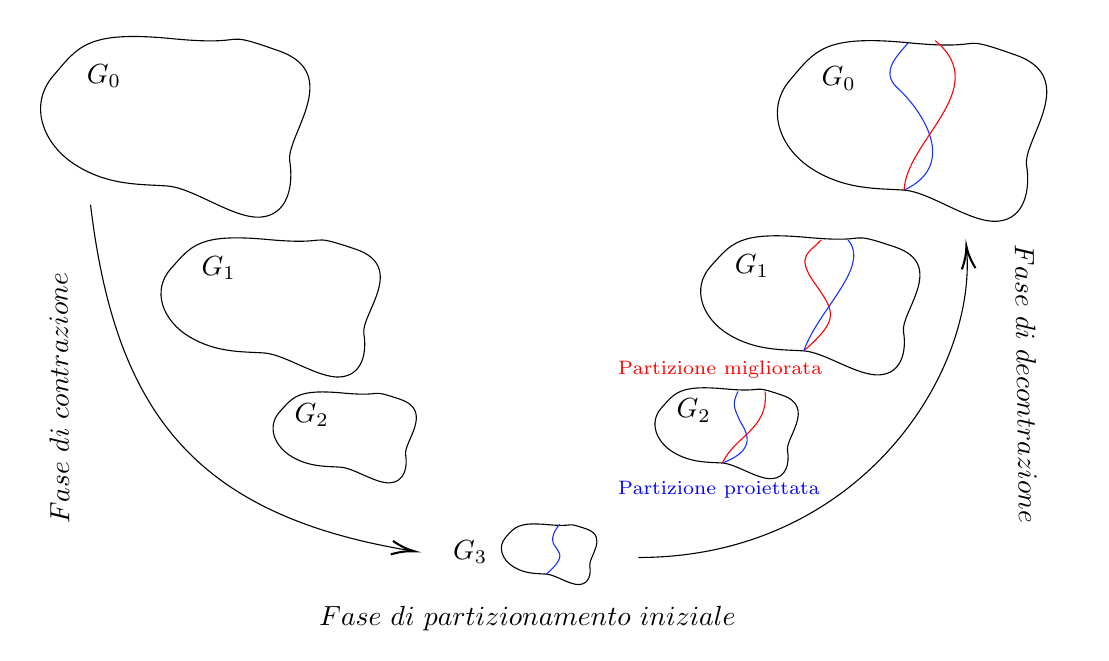
\begin{tikzpicture}[x=0.75pt,y=0.75pt,yscale=-1,xscale=1]
%uncomment if require: \path (0,301); %set diagram left start at 0, and has height of 301

%Shape: Polygon Curved [id:ds5681990127641572]
\draw   (13,23) .. controls (25,9) and (29,1) .. (70,5) .. controls (111,9) and (91,0) .. (122,11) .. controls (153,22) and (125.09,51.89) .. (127,64) .. controls (128.91,76.11) and (126,90) .. (113,91) .. controls (100,92) and (80.66,76.9) .. (68,76) .. controls (55.34,75.1) and (40,76) .. (24,66) .. controls (8,56) and (1,37) .. (13,23) -- cycle ;
%Shape: Polygon Curved [id:ds5791880784550985]
\draw   (69.88,115.65) .. controls (79.65,104.87) and (82.9,98.71) .. (116.29,101.79) .. controls (149.67,104.87) and (133.38,97.94) .. (158.63,106.41) .. controls (183.87,114.88) and (161.14,137.9) .. (162.7,147.22) .. controls (164.25,156.55) and (161.88,167.24) .. (151.3,168.01) .. controls (140.71,168.78) and (124.96,157.16) .. (114.66,156.46) .. controls (104.35,155.77) and (91.86,156.46) .. (78.83,148.76) .. controls (65.81,141.06) and (60.11,126.43) .. (69.88,115.65) -- cycle ;
%Shape: Polygon Curved [id:ds8471099289598505]
\draw   (122.17,184.81) .. controls (128.56,177.76) and (130.68,173.74) .. (152.5,175.75) .. controls (174.32,177.76) and (163.67,173.23) .. (180.17,178.77) .. controls (196.67,184.3) and (181.81,199.34) .. (182.83,205.44) .. controls (183.85,211.53) and (182.3,218.52) .. (175.38,219.02) .. controls (168.46,219.53) and (158.17,211.93) .. (151.44,211.48) .. controls (144.7,211.02) and (136.54,211.48) .. (128.02,206.44) .. controls (119.51,201.41) and (115.79,191.85) .. (122.17,184.81) -- cycle ;
%Shape: Polygon Curved [id:ds042557391147138635]
\draw   (231.1,245.21) .. controls (235.36,240.51) and (236.78,237.83) .. (251.33,239.17) .. controls (265.87,240.51) and (258.78,237.49) .. (269.78,241.19) .. controls (280.78,244.88) and (270.87,254.91) .. (271.55,258.97) .. controls (272.23,263.04) and (271.2,267.7) .. (266.58,268.03) .. controls (261.97,268.37) and (255.11,263.3) .. (250.62,263) .. controls (246.13,262.69) and (240.68,263) .. (235,259.64) .. controls (229.32,256.29) and (226.84,249.91) .. (231.1,245.21) -- cycle ;
%Shape: Polygon Curved [id:ds19971791116540039]
\draw   (368,25) .. controls (380,11) and (384,3) .. (425,7) .. controls (466,11) and (446,2) .. (477,13) .. controls (508,24) and (480.09,53.89) .. (482,66) .. controls (483.91,78.11) and (481,92) .. (468,93) .. controls (455,94) and (435.66,78.9) .. (423,78) .. controls (410.34,77.1) and (395,78) .. (379,68) .. controls (363,58) and (356,39) .. (368,25) -- cycle ;
%Shape: Polygon Curved [id:ds6697871941207159]
\draw   (329.88,114.65) .. controls (339.65,103.87) and (342.9,97.71) .. (376.29,100.79) .. controls (409.67,103.87) and (393.38,96.94) .. (418.63,105.41) .. controls (443.87,113.88) and (421.14,136.9) .. (422.7,146.22) .. controls (424.25,155.55) and (421.88,166.24) .. (411.3,167.01) .. controls (400.71,167.78) and (384.96,156.16) .. (374.66,155.46) .. controls (364.35,154.77) and (351.86,155.46) .. (338.83,147.76) .. controls (325.81,140.06) and (320.11,125.43) .. (329.88,114.65) -- cycle ;
%Shape: Polygon Curved [id:ds6317966254041107]
\draw   (306.17,182.81) .. controls (312.56,175.76) and (314.68,171.74) .. (336.5,173.75) .. controls (358.32,175.76) and (347.67,171.23) .. (364.17,176.77) .. controls (380.67,182.3) and (365.81,197.34) .. (366.83,203.44) .. controls (367.85,209.53) and (366.3,216.52) .. (359.38,217.02) .. controls (352.46,217.53) and (342.17,209.93) .. (335.44,209.48) .. controls (328.7,209.02) and (320.54,209.48) .. (312.02,204.44) .. controls (303.51,199.41) and (299.79,189.85) .. (306.17,182.81) -- cycle ;
%Curve Lines [id:da4556621139317687]
\draw [color={rgb, 255:red, 0; green, 0; blue, 255 }  ,draw opacity=1 ]   (250.62,263) .. controls (267,249) and (246,253) .. (257,239) ;
%Curve Lines [id:da3153745771749539]
\draw [color={rgb, 255:red, 0; green, 0; blue, 255 }  ,draw opacity=1 ]   (335.44,209.48) .. controls (355,202) and (345.05,192.39) .. (343.35,188.03) .. controls (341.65,183.68) and (339.62,181.49) .. (343,175) ;
%Curve Lines [id:da24590148322887484]
\draw [color={rgb, 255:red, 255; green, 0; blue, 0 }  ,draw opacity=1 ]   (335.44,209.48) .. controls (341.44,196.48) and (358,193) .. (356,175) ;
%Curve Lines [id:da8069367964557173]
\draw [color={rgb, 255:red, 255; green, 0; blue, 0 }  ,draw opacity=1 ]   (374.66,155.46) .. controls (391.66,140.46) and (390,137) .. (380,123) .. controls (370,109) and (378,108) .. (383,102) ;
%Curve Lines [id:da030698152549456736]
\draw [color={rgb, 255:red, 0; green, 0; blue, 255 }  ,draw opacity=1 ]   (374.66,155.46) .. controls (381.66,135.46) and (407,115) .. (396,102) ;
%Curve Lines [id:da9188529841976845]
\draw [color={rgb, 255:red, 0; green, 0; blue, 255 }  ,draw opacity=1 ]   (423,78) .. controls (451,65) and (429,37) .. (420,29) .. controls (411,21) and (420,13) .. (425,7) ;
%Curve Lines [id:da500049878186364]
\draw [color={rgb, 255:red, 255; green, 0; blue, 0 }  ,draw opacity=1 ]   (423,78) .. controls (424,54) and (466,29) .. (438,6) ;
%Curve Lines [id:da5337953441131338]
\draw    (31,85) .. controls (42.94,184.5) and (80.62,234.5) .. (185.42,251.74) ;
\draw [shift={(187,252)}, rotate = 189.11] [color={rgb, 255:red, 0; green, 0; blue, 0 }  ][line width=0.75]    (10.93,-3.29) .. controls (6.95,-1.4) and (3.31,-0.3) .. (0,0) .. controls (3.31,0.3) and (6.95,1.4) .. (10.93,3.29)   ;
%Curve Lines [id:da17376352225172775]
\draw    (295,255) .. controls (400.93,255) and (457.86,166.79) .. (453.16,106.81) ;
\draw [shift={(453,105)}, rotate = 84.29] [color={rgb, 255:red, 0; green, 0; blue, 0 }  ][line width=0.75]    (10.93,-3.29) .. controls (6.95,-1.4) and (3.31,-0.3) .. (0,0) .. controls (3.31,0.3) and (6.95,1.4) .. (10.93,3.29)   ;

% Text Node
\draw (28,16.4) node [anchor=north west][inner sep=0.75pt]    {$G_{0}$};
% Text Node
\draw (83.23,108.82) node [anchor=north west][inner sep=0.75pt]    {$G_{1}$};
% Text Node
\draw (128.13,179.36) node [anchor=north west][inner sep=0.75pt]    {$G_{2}$};
% Text Node
\draw (204.41,245.38) node [anchor=north west][inner sep=0.75pt]    {$G_{3}$};
% Text Node
\draw (382,17.4) node [anchor=north west][inner sep=0.75pt]    {$G_{0}$};
% Text Node
\draw (340.23,107.82) node [anchor=north west][inner sep=0.75pt]    {$G_{1}$};
% Text Node
\draw (312.13,177.36) node [anchor=north west][inner sep=0.75pt]    {$G_{2}$};
% Text Node
\draw (10.34,240.07) node [anchor=north west][inner sep=0.75pt]  [rotate=-269.56]  {$Fase\ di\ contrazione$};
% Text Node
\draw (486.92,102.91) node [anchor=north west][inner sep=0.75pt]  [rotate=-89.15]  {$Fase\ di\ decontrazione$};
% Text Node
\draw (140,277.4) node [anchor=north west][inner sep=0.75pt]    {$Fase\ di\ partizionamento\ iniziale$};
% Text Node
\draw (284,217) node [anchor=north west][inner sep=0.75pt]   [align=left] {{\scriptsize \textcolor[rgb]{0,0,1}{Partizione proiettata}}};
% Text Node
\draw (284,159) node [anchor=north west][inner sep=0.75pt]  [font=\normalsize] [align=left] {{\scriptsize \textcolor[rgb]{1,0,0}{Partizione migliorata}}};


\end{tikzpicture}

    \caption{Schema grafico del partizionamento multi-livello}
    \label{fig:multi-level-graph-partitioning}
\end{figure}

L'approccio multi-livello per la partizione di grafi si articola in tre fasi principali:
\begin{enumerate}
    \item \textbf{Fase di contrazione} (\textit{contraction/coarsening phase}):
    si crea una gerarchia di grafi riducendo iterativamente la dimensione del grafo iniziale.
    Questo viene fatto comunemente individuando e contraendo coppie di nodi adiacenti, ovvero individuando un
    sottoinsieme degli archi del grafo da contrarre, $M \subseteq E $ detti \textit{match}.
    Si noti che la scelta di contrarre coppie di nodi adiacenti porta a grafi grossolani i cui nodi rappresentano
    sottografi del grafo iniziale densamente connessi.
    In base allo specifico problema, una determinata funzione di \textit{rating} classifica gli archi individuando
    quale sottoinsieme degli archi $E$ debba essere assegnato ad $M$ affinch\`e la somma dei \textit{rating} degli in
    $M$ sia globalmente massimizzata.
    Si consideri che un nodo gi\`a contratto non pu\`o essere pi\`u coinvolto in un ulteriore \textit{matching}
    allo stesso livello della gerarchia.
    \item \textbf{Fase di partizionamento iniziale} (\textit{initial partitioning phase}): quando a seguito delle
    contrazioni il grafo risulta essere di ordine abbastanza piccolo, in relazione ad un qualche threshold,
    esso pu\`o essere partizionato direttamente con algoritmi costosi, fornendo una partizione iniziale sul grafo
    pi\`u grossolano della gerarchia.
    \item \textbf{Fase di decontrazione} (\textit{refinement/uncoarsening phase}), i matching vengono iterativamente
    decontratti, e i relativi nodi vengono associati a blocchi della partizione del grafo pi\`u grossolano,
    proiettandola sul grafo pi\`u raffinato.
    Per fare in modo che la partizione al livello pi\`u grossolano tenga conto delle sotto-strutture ai livelli
    pi\`u raffinati, un algoritmo di miglioramento locale (\textit{local improvement}) ricolloca i nodi tra i
    blocchi per migliorare la dimensione del taglio o l'equilibrio delle dimensioni tra i blocchi.
\end{enumerate}





\chapter{Grafi Multi-livello}\label{cap:grafi-multi-livello}

Come si \`e potuto vedere dal contenuto del Capitolo~\ref{cap:grafi-e-approccio-multi-livello},
le operazioni di contrazione e la costruzione di
gerarchie di grafi a pi\`u livelli siano concetti gi\`a ampiamente utilizzati e consolidati nella teoria dei grafi e
nelle sue applicazioni.
Tuttavia, ci\`o che non \`e stato ancora propriamente considerato nella letteratura esistente \`e la possibilit\`a di
definire e formalizzare una vera e propria struttura dati astratta che rappresenti un grafo multi-livello come
un'entit\`a a s\`e stante.
In questo capitolo verranno date le fondamenta per la definizione del concetto di \textit{Grafo Multi-livello} dal
punto di vista algebrico, e verranno introdotte le operazioni di base che permetteranno di rendere
algoritmicamente realizzabile la costruzione di tale struttura dati.

\section{Definizioni e propriet\`a di base}\label{sec:definizioni-e-proprieta-di-base}

In questa sezione saranno proposte definizioni e propriet\`a di base di una struttura dati per la rappresentazione
di gerarchie di grafi a pi\`u livelli, in cui sia possibile ottenere informazioni sull'intera struttura gerarchica in
relazione ai singoli grafi che la compongono, come attraverso l'espansione e la contrazione di nodi.
In particolare, riprendendo dalla terminologia e dai concetti esistenti in letteratura, si proporranno definizioni
originali di \textit{grafo decontraibile} e di \textit{grafo multi-livello}.

\subsection{Grafo decontraibile}

A partire dal concetto noto di grafo quoziente e di contrazione, si vuole definire una particolare
tipologia di grafi quoziente che, oltre a rappresentare le caratteristiche strutturali ad alto livello di astrazione
dei grafi da cui sono derivati, siano in grado di mantenere l'informazione originale di questi ultimi, in
che modo essa sia legata alla sua rappresentazione astratta. \newline
Nasce così il concetto di grafo decontraibile, che intuitivamente pu\`o essere considerato come un grafo
in cui i nodi sono riconducibili ad un grafo e gli archi ad un insieme di archi tra i nodi dei grafi
associati ai nodi coinvolti.
\newpage

\begin{definition}[Grafo decontraibile]
    Un \textbf{grafo decontraibile} $G$ \`e una quadrupla $(V, E, dec_V, dec_E)$ dove:
    \begin{itemize}
        \item $V$ \`e un insieme di elementi detti \textbf{supernodi};
        \item $E \subseteq V \times V$ \`e un insieme di coppie ordinate di supernodi, dette \textbf{superarchi};
        \item $dec_V : V \rightarrow \mathcal{G}_D$ \`e una funzione tale per cui $dec_V(v) = (\mathcal{V}_v,
            \mathcal{E}_v, dec_{\mathcal{V}_v}, dec_{\mathcal{E}_v})$ \`e un grafo decontraibile rappresentato
            dal supernodo $v$;
        \item $dec_E : E \rightarrow (\mathcal{V} \times \mathcal{V})$ con $\mathcal{V} = \bigcup_{v \in V}\mathcal{V}_v$,
            \`e una funzione tale per cui $\forall$ $ e = (u, v)$, \\ $dec_E(e) = \mathcal{E}_e \subseteq$ $\{(a, b)$ $\mid$ $a \in \mathcal{V}_u$ $\wedge$
            $b \in \mathcal{V}_v\}$ \`e un insieme di archi rappresentati dal superarco $e$.
    \end{itemize}
\end{definition}

Nella definizione, cos\`{i} come d'ora in avanti, si utilizzer\`a la notazione $\mathcal{G}_D$ per indicare l'insieme
dei grafi decontraibili, e le notazioni $\mathcal{V}$ e $\mathcal{E}$ per
indicare, rispettivamente, insiemi di supernodi e superarchi ottenibili attraverso decontrazioni e, quindi, di
livello inferiore rispetto al grafo decontratto di riferimento.
Le notazioni $\mathcal{V}_v$ e $\mathcal{E}_v$ saranno utilizzate per indicare, rispettivamente,
insiemi di nodi e archi di grafi ottenibili attraverso la decontrazione di un certo supernodo $v$.
Nel contesto di un determinato grafo decontraibile, per portare maggiore distinzione si continuer\`a ad utilizzare
il termine di nodo ed arco per riferirsi ai supernodi e superarchi di tale livello inferiore. \newline

Si noti che \`e possibile usare una notazione basata su attributi, alternativa a quella delle funzioni, per
descrivere le propriet\`a caratteristiche di nodi ed archi che rendono tale un grafo decontraibile.
Tale notazione sar\`a utilizzata in seguito per semplificare la descrizione di algoritmi. \newline
In particolare, si pu\`o definire un grafo decontraibile come un normale grafo diretto sotto forma di coppia
$(V, E)$ dove:
\begin{itemize}
    \item $\forall$ $v \in V,$ \`e definito un attributo $v.dec = G_v$ dove $G_v = (\mathcal{V}_v, \mathcal{E}_v)$ \`e un
        grafo decontraibile rappresentato da $v$, quindi tale per cui $dec_V(v) = v.dec$.
    \item $\forall$ $e=(u, v)$  $\in E$, \`e definito una attributo $e.dec = E_e$ dove \\
        ${\mathcal{E}_e \subseteq \{(a, b) \mid a \in \mathcal{V}_u \wedge b \in \mathcal{V}_v\}}$ \`e un insieme di archi
        rappresentati da $e$, quindi tale per cui $dec_E(e) = e.dec$.
\end{itemize}

Si consideri la natura ricorsiva definizione di grafo decontraibile, per cui se un supernodo $v$ pu\`o essere
rappresentato da un grafo decontraibile $G_v$, allora i nodi di $G_v$ saranno a loro volta dei supernodi.
Stessa cosa vale per gli archi, che possono essere rappresentati da insiemi di archi tra i nodi dei grafi.
La scelta di rendere il grafo decontraibile una struttura ricorsiva, cos\`{i} come la definizione in sé stessa,
\`e utile alle successive definizioni legate ai grafi multi-livello. \newline

\begin{figure}[h!]
\centering
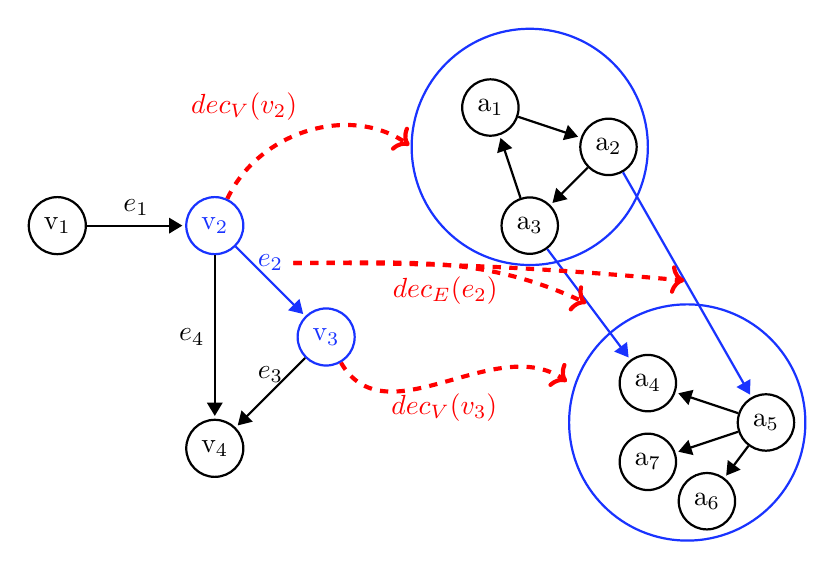
\begin{tikzpicture}
  [mynode/.style={draw, thick, circle, size=0.3mm},
    myarrow/.style={thick, -Triangle},
    ->,shorten >=1pt,auto,node distance=2cm, thick,main node/.style={circle,draw}]

  % Nodes
  \node[main node] (A) {v$_1$};
  \node[main node, blue] (B) [right of=A] {v$_2$};
  \node[main node, blue] (C) [below right of=B] {v$_3$};
  \node[main node] (D) [below left of=C] {v$_4$};

  % Edges
  \path[every node/.style={font=\sffamily\small}];
  \draw[myarrow](A) to node [above] {$e_1$} (B);
  \draw[myarrow, blue] (B) to node [above, name=e2] {$e_2$} (C);
  \draw[myarrow](C) to node [above] {$e_3$} (D);
  \draw[myarrow](B) to node [left] {$e_4$} (D);

  % G_b graph
  \begin{scope}[shift={(6,1)}]
  \draw[blue] (0,0) circle (1.5cm);
  \node[main node] (X) at (-0.5,0.5) {a$_1$};
  \node[main node] (Y) at (1,0) {a$_2$};
  \node[main node] (Z) at (0,-1) {a$_3$};
  \draw[myarrow] (X) -- (Y);
  \draw[myarrow] (Y) -- (Z);
  \draw[myarrow] (Z) -- (X);
  \end{scope}

  % G_c graph
  \begin{scope}[shift={(8,-2.5)}]
  \draw[blue] (0,0) circle (1.5cm);
  \node[main node] (T) at (-0.5,0.5) {a$_4$};
  \node[main node] (U) at (1,0) {a$_5$};
  \node[main node] (V) at (0.25,-1) {a$_6$};
  \node[main node] (W) at (-0.5,-0.5) {a$_7$};
  \draw[myarrow] (U) -- (T);
  \draw[myarrow] (U) -- (W);
  \draw[myarrow] (U) -- (V);
  \end{scope}

  % edges between graphs
  \draw[myarrow, blue] (Z) -- (T);
  \draw[myarrow, blue] (Y) -- (U);

  % Links
  \draw[dashed, line width=1.5pt, red] (B) to[out=65, in=145] node {$dec_{V}(v_2)$} (4.5,1);
  \draw[dashed, line width=1.5pt, red] (e2) to[out=0, in=155] node [below] {$dec_{E}(e_2)$} (6.75,-1);
  \draw[dashed, line width=1.5pt, red] (e2) to[out=0, in=175] (8,-0.7);
  \draw[dashed, line width=1.5pt, red] (C) to[out=300, in=145] node [below] {$dec_{V}(v_3)$} (6.5,-2);
\end{tikzpicture}
\vspace{-15pt}
\caption{Un esempio di decontrazione locale di un grafo decontraibile}
\label{fig:dec-graph-example}
\end{figure}

In Figura~\ref{fig:dec-graph-example} \`e mostrato un esempio di grafo decontraibile sulla sinistra, mentre sulla
destra sono rappresentati i grafi associati ai supernodi $v_2$ e $v_3$, assieme all'insieme di archi associato
al superarco $e_2$.
Si osservi che il grafo $dec_V(v_2)$ composto dai nodi $a_1$, $a_2$ e $a_3$, ad esempio, manca degli archi collegati
esternamente che definiscono il contesto in cui tale grafo si colloca, e solo uno degli archi incidenti
in $v_1$ \`e stato espanso.
Questo fornisce una visione parziale dell'informazione contenuta nel grafo decontraibile a sinistra,
e per questo si pu\`o dire che il grafo a destra \`e il risultato di un'espansione locale. \newline

Inoltre, dal momento in cui i grafi decontraibili sono a tutti gli effetti dei grafi, tutte le
definizioni date sui grafi standard continuano ad essere utilizzate in modo equivalente per i grafi decontraibili.
Analogamente, un supernodo pu\`o essere considerato come un particolare tipo di nodo, e lo stesso vale per i
superarchi.
In particolare, il concetto di isomorfismo pu\`o essere esteso ai grafi decontraibili senza particolari modifiche,
ignorando l'aspetto ``decontraibile'' di nodi e archi, ovvero ignorando le funzioni $dec_V$ e $dec_E$ di entrambi
i grafi di cui si vuole valutare l'isomorfismo.

% Potrebbe essere altres\`{i} utile indicare un tipo di isomorfismo specifico per i grafi decontraibili, che tenga
% conto delle funzioni di decontrazione, ovvero che imponga un isomorfismo anche tra i grafi risultanti dalle
% decontrazioni dei singoli nodi, risultando in una forma di isomorfismo pi\`u forte.

% \begin{defintion}[Isomorfismo forte di Grafi Decontraibili] \newline
%    Siano $G = (V, E)$ e $H = (W, F)$ due grafi decontraibili, essi si dicono \textbf{fortemente isomorfi} se
%     esiste una biiezione $f : V \rightarrow W$ tale per cui
%     \begin{itemize}
%        \item $(u, v) \in E$ se e solo se $(f(u), f(v)) \in F$ per ogni $u, v \in V$
%        \item $dec_V(u)$ \`e fortemente isomorfo a $dec_V(f(u))$ per ogni $u \in V$
%        \item
%    \end{itemize}

%\end{defintion}

\nlparagraph{Contrazioni di grafi decontraibili}\label{subsec:contrazioni}

A partire dalla decontrazione, che rappresenta un aspetto intrinseco alla definizione dei grafi decontraibili,
la relazione di contrazione \`e quella che, intuitivamente, permette di legare grafi decontraibili nel senso
opposto.
Se da un lato la decontrazione permette di costruire grafi che rappresentino espansioni locali, con una
definizione di contrazione si vogliono stabilire le condizioni che permettono di legare interi grafi decontraibili
ad altri che ne forniscano una loro rappresentazione astratta, affinch\`e la tale rappresentazione
sia coerente con il concetto di contrazione esistente nella teoria dei grafi.

\begin{definition}[Contrazione di un grafo decontraibile]
    Sia $G = (V, E, dec_V, dec_E)$ un grafo decontraibile, il grafo decontraibile \\
    $G\mathcal{'} = (\mathfrak{V}, \mathfrak{E}, dec_{\mathfrak{V}}, dec_{\mathfrak{E}})$ \`e una sua
    \textbf{contrazione} se e solamente se:
        \begin{itemize}
            \item l'insieme $\{V_\alpha \mid \alpha \in \mathfrak{V}\}$ \`e una partizione di $V$;
            \item l'insieme $(\{E_\alpha \mid \alpha \in \mathfrak{V}\} \setminus \{ \emptyset \}) \cup
                \{ dec_{\mathfrak{E}}(\epsilon) \mid \epsilon \in \mathfrak{E}\}$ \`e una partizione di $E$.
        \end{itemize}
\end{definition}

Nella definizione, cos\`{i} come d'ora in avanti, si utilizzer\`a la notazione $\mathfrak{V}$ e $\mathfrak{E}$ per
indicare, rispettivamente, gli insiemi di supernodi e superarchi di un grafo contratto, e quindi di livello
superiore rispetto al grafo di riferimento.

Nella Figura~\ref{fig:contraction-example}, sulla sinistra \`e mostrato un esempio di grafo decontraibile
contrazione del grafo decontraibile a destra, dove sono annotati per ogni supernodo e superarco
i nodi e gli archi ottenibili dalle loro decontrazioni. \newline

\begin{figure}
    \centering
    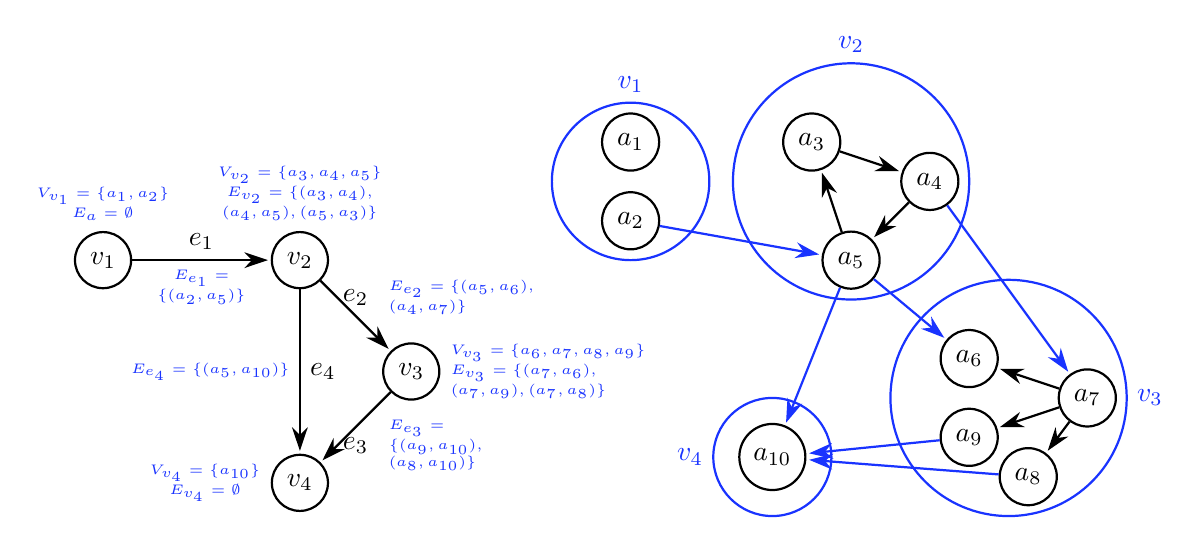
\begin{tikzpicture}
    [mynode/.style={draw, thick, circle, size=0.3mm},
    ->,shorten >=1pt,auto,node distance=2cm, thick, main node/.style={circle,draw}]

        % Nodes
        \node[main node,
          label={[align=center, blue, font=\tiny]above:{$V_{v_1} = \{a_1, a_2\}$}\\{$E_a = \emptyset$}}]
        (A) {$v_1$};
        \node[main node,
        label={[align=center, blue, font=\tiny]above:{$V_{v_2} = \{a_3, a_4, a_5\}$}\\{$E_{v_2} = \{(a_3, a_4),$}\\{$(a_4, a_5), (a_5, a_3)\}$}}]
        (B) [right of=A, node distance=2.5cm] {$v_2$};
        \node[main node,
        label={[align=left, blue, font=\tiny]right:{$V_{v_3} = \{a_6, a_7, a_8, a_9\}$}\\{$E_{v_3} = \{(a_7, a_6),$}\\{$(a_7, a_9),(a_7, a_8)\}$}}]
          (C) [below right of=B] {$v_3$};
        \node[main node,
        label={[align=center, blue, font=\tiny]left:{$V_{v_4} = \{a_{10}\}$}\\{$E_{v_4} = \emptyset$}}]
          (D) [below left of=C] {$v_4$};

        % Edges
        \path[every node/.style={font=\sffamily\small}];
        \draw[myarrow](A) to node [above,
        label={[align=center, blue, font=\tiny]below:{$E_{e_1} = $}\\{$\{(a_2, a_5)\}$}}] {$e_1$} (B);
        \draw[myarrow](B) to node [above,
        label={[align=left, blue, font=\tiny]right:{$E_{e_2} = \{(a_5,a_6),$}\\{$(a_4, a_7)\}$}}] {$e_2$} (C);
        \draw[myarrow](C) to node [below,
        label={[align=left, blue, font=\tiny]right:{$E_{e_3} =$}\\{$ \{(a_9,a_{10}),$}\\{$ (a_8, a_{10})\}$}}] {$e_3$} (D);
        \draw[myarrow](B) to node [right, label={[align=right, blue, font=\tiny]left:{$E_{e_4} = \{(a_5,a_{10})\}$}}] {$e_4$} (D);

        % G_b graph
        \begin{scope}[shift={(9.5,1)}];
        \draw[blue] (0,0) circle (1.5cm);
        \node[above, blue] at (0,1.5) {$v_2$};
        \node[main node] (X) at (-0.5,0.5) {$a_3$};
        \node[main node] (Y) at (1,0) {$a_4$};
        \node[main node] (Z) at (0,-1) {$a_5$};
        \draw[myarrow] (X) -- (Y);
        \draw[myarrow] (Y) -- (Z);
        \draw[myarrow] (Z) -- (X);
        \end{scope}

        % G_c graph
        \begin{scope}[shift={(11.5,-1.75)}]
        \draw[blue] (0,0) circle (1.5cm);
        \node[right, blue] at (1.5,0) {$v_3$};
        \node[main node] (T) at (-0.5,0.5) {$a_6$};
        \node[main node] (U) at (1,0) {$a_7$};
        \node[main node] (V) at (0.25,-1) {$a_8$};
        \node[main node] (W) at (-0.5,-0.5) {$a_9$};
        \draw[myarrow] (U) -- (T);
        \draw[myarrow] (U) -- (W);
        \draw[myarrow] (U) -- (V);
        \end{scope}

        % G_a graph
        \begin{scope}[shift={(6.7, 1)}]
        \draw[blue] (0,0) circle (1cm);
        \node[above, blue] at (0,1) {$v_1$};
        \node[main node] (N) at (0,0.5) {$a_1$};
        \node[main node] (M) at (0,-0.5) {$a_2$};
        \end{scope}

        % G_d graph
        \begin{scope}[shift={(8.5,-2.5)}]
        \draw[blue] (0,0) circle (0.75cm);
        \node[left, blue] at (-0.75,0) {$v_4$};
        \node[main node] (K) at (0,0) {$a_{10}$};
        \end{scope}

        % edges between graphs
        \draw[myarrow, blue] (M) -- (Z);
        \draw[myarrow, blue] (Z) -- (K);
        \draw[myarrow, blue] (Z) -- (T);
        \draw[myarrow, blue] (Y) -- (U);
        \draw[myarrow, blue] (W) -- (K);
        \draw[myarrow, blue] (V) -- (K);
\end{tikzpicture}
    \caption{Esempio di contrazione di un grafo decontraibile}
    \label{fig:contraction-example}
\end{figure}

Dalla definizione si evince che le seguenti sono condizioni necessarie affinch\`e un grafo decontraibile $G'$ possa
essere una contrazione di un grafo decontraibile $G$:
\begin{enumerate}[(i)]
    \item I nodi di $G'$ devono avere tutti un grafo non vuoto come decontrazione, ovvero $V_\alpha \neq \emptyset$
    per ogni $\alpha \in \mathfrak{V}$.
    Infatti se fosse che $V_\alpha = \emptyset$ per qualche $\alpha \in \mathfrak{V}$, allora l'insieme
    $\{V_\alpha \mid \alpha \in \mathfrak{V}\}$ non costituirebbe una partizione di $V$, in quanto, per definizione,
    l'insieme vuoto non pu\`o essere incluso in una partizione.
    \item Gli insiemi di nodi delle decontrazioni dei supernodi in $G'$ devono essere a due a due disgiunti, ovvero
    non possono esistere nodi a cui corrispondono contemporaneamente due supernodi distinti, in quanto, anche in
    questo caso, l'insieme $\{V_\alpha \mid \alpha \in \mathfrak{V}\}$ non costituirebbe una partizione di $V$.
    \item I superarchi di $G'$ devono avere tutti una decontrazione non vuota.
    Infatti, se fosse che $dec_{\mathfrak{E}}(\epsilon) = \emptyset$ per qualche $\epsilon \in \mathfrak{E}$, allora
    l' insieme $(\{E_\alpha \mid \alpha \in \mathfrak{V}\} \setminus \{ \emptyset \}) \cup
    \{ dec_{\mathfrak{E}}(\epsilon) \mid \epsilon \in \mathfrak{E}\}$ non costituirebbe una partizione di $E$,
    analogamente a quanto detto nel punto (i). \newline
    Si noti che la condizione di disgiunzione tra gli insiemi di archi delle decontrazioni dei superarchi \`e
    automaticamente soddisfatta dalla definizione di grafo decontraibile e delle decontrazioni dei suoi archi.
\end{enumerate}

E' rilevante notare che, data una contrazione $G'$ del grafo decontraibile $G$, essa contiene tutte le informazioni
necessarie a calcolare la struttura di archi e nodi di $G$.
Infatti, sia $G' = (\mathfrak{V}, \mathfrak{E})$ una contrazione di $G$, allora dalla definizione si ha:

\begin{equation*}
    G = (\bigcup_{\alpha \in \mathfrak{V}} V_\alpha , \;
        (\bigcup_{\alpha \in \mathfrak{V}} E_\alpha \cup \bigcup_{\epsilon \in \mathfrak{E}}{dec_{\mathfrak{E}}(\epsilon)}), \;
        dev_V, \; dec_E) %TODO: \bigsqcup{\alpha \in \mathfrak{V}} dec_{V_{\alpha}}, (\bigsqcup{\alpha \in \mathfrak{V}} dec_{E_{\alpha}} \cup ???)
\end{equation*}

dove $dec_V$ è ottenuto dall'unione delle funzioni $dec_{\mathfrak{V}_v}$ per ciascun $v \in \mathfrak{V}$,
e $dec_E$ è ottenuto dall'unione delle funzioni $dec_{\mathfrak{E}_e}$ per ciascun $e \in \mathfrak{E}$ combinato con
tutte le mappature tra i superarchi in $\bigcup{\epsilon \in \mathfrak{E}} dec_{\mathfrak{E}}(\epsilon)$ e le loro
decontrazioni. \newline

Definiamo, quindi, l'operatore unario $.^D : \mathcal{G}_D \rightarrow \mathcal{G}_D$ come l'operatore di
\textbf{decontrazione completa} che, dato un grafo decontraibile $G = (V, E, dec_V, dec_E)$ restituisce il grafo
decontraibile $G^D$ ottenuto dalla decontrazione di tutti i supernodi e superarchi del grafo in input.

\begin{equation*}
    G^D = (\bigcup_{v \in V} \mathcal{V}_v , \; (\bigcup_{v \in V} \mathcal{E}_v \cup \bigcup_{e \in E} dec_E(e)), \;
    dec_{\mathcal{V}}, \; dec_{\mathcal{E}})
\end{equation*}

Una contrazione di un grafo decontraibile $G$ pu\`o, quindi, essere alternativamente definita come un suo grafo
quoziente decontraibile $G'$ la cui decontrazione completa $(G')^D$ \`e proprio $G$.
\newline

Si noti che, in generale, un grafo decontraibile $G$ pu\`o non essere una contrazione di $G^D$.
Questo pu\`o verificarsi unicamente quando $G$ non soddisfa tutte le condizioni (i), (ii) e (iii) presentate in
precedenza. \newline
Per rendere chiaro questo aspetto, in Figura~\ref{fig:non-contraction-example} \`e proposta una variazione
dell'esempio precedente, in cui il grafo decontraibile a sinistra, ottenuto come decontrazione completa del grafo
destra, non \`e una sua contrazione, in quanto il super-nodo $a_3$ appartiene contemporaneamente a $V_a$ e $V_b$,
violando la condizione (ii), e il super-arco $e_3$ viene decontratto in un insieme vuoto di archi,
violando la condizione (iii).

\begin{figure}
    \centering
    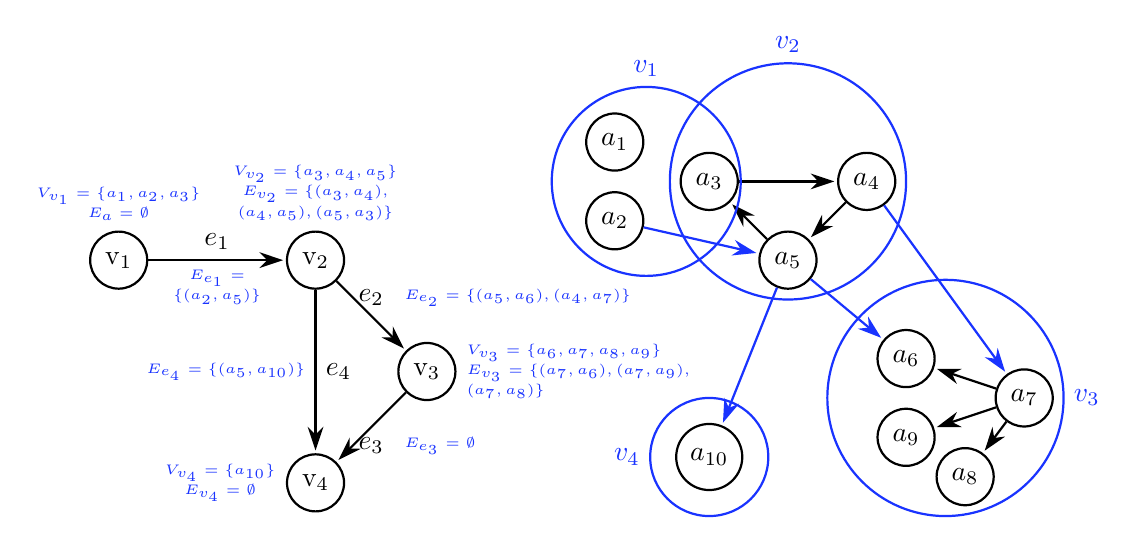
\begin{tikzpicture} [mynode/.style={draw, thick, circle, minimum size=0.3cm},
    ->,>={stealth},shorten >=1pt,auto,node distance=2cm,
    thick,main node/.style={circle,draw}]

    % Nodes
    \node[main node,
        label={[align=center, blue, font=\tiny]above:{$V_{v_1} = \{a_1, a_2, a_3\}$}\\{$E_a = \emptyset$}}]
    (A) {v$_1$};
    \node[main node,
        label={[align=center, blue, font=\tiny]above:{$V_{v_2} = \{a_3, a_4, a_5\}$}\\{$E_{v_2} = \{(a_3, a_4),$}\\{$(a_4, a_5), (a_5, a_3)\}$}}]
    (B) [right of=A, node distance=2.5cm] {v$_2$};
    \node[main node,
        label={[align=left, blue, font=\tiny]right:{$V_{v_3} = \{a_6, a_7, a_8, a_9\}$}\\{$E_{v_3} = \{(a_7, a_6),(a_7, a_9),$}\\{$(a_7, a_8)\}$}}]
    (C) [below right of=B] {v$_3$};
    \node[main node,
        label={[align=center, blue, font=\tiny]left:{$V_{v_4} = \{a_{10}\}$}\\{$E_{v_4} = \emptyset$}}]
    (D) [below left of=C] {v$_4$};

    % Edges
    \path[every node/.style={font=\sffamily\small}];
    \draw[myarrow](A) to node [above,
    label={[align=center, blue, font=\tiny]below:{$E_{e_1} = $}\\{$\{(a_2, a_5)\}$}}] {$e_1$} (B);
    \draw[myarrow](B) to node [above,
    label={[align=left, blue, font=\tiny]right:{$E_{e_2} = \{(a_5,a_6), (a_4, a_7)\}$}}] {$e_2$} (C);
    \draw[myarrow](C) to node [below,
    label={[align=left, blue, font=\tiny]right:{$E_{e_3} = \emptyset$}}] {$e_3$} (D);
    \draw[myarrow](B) to node [right, label={[align=right, blue, font=\tiny]left:{$E_{e_4} = \{(a_5,a_{10})\}$}}] {$e_4$} (D);

    % G_b graph
    \begin{scope}[shift={(8.5,1)}]
    \draw[blue] (0,0) circle (1.5cm);
    \node[above, blue] at (0,1.5) {$v_2$};
    \node[main node] (X) at (-1,0) {$a_3$};
    \node[main node] (Y) at (1,0) {$a_4$};
    \node[main node] (Z) at (0,-1) {$a_5$};
    \draw[myarrow] (X) -- (Y);
    \draw[myarrow] (Y) -- (Z);
    \draw[myarrow] (Z) -- (X);
    \end{scope}

    % G_c graph
    \begin{scope}[shift={(10.5,-1.75)}]
    \draw[blue] (0,0) circle (1.5cm);
    \node[right, blue] at (1.5,0) {$v_3$};
    \node[main node] (T) at (-0.5,0.5) {$a_6$};
    \node[main node] (U) at (1,0) {$a_7$};
    \node[main node] (V) at (0.25,-1) {$a_8$};
    \node[main node] (W) at (-0.5,-0.5) {$a_9$};
    \draw[myarrow] (U) -- (T);
    \draw[myarrow] (U) -- (W);
    \draw[myarrow] (U) -- (V);
    \end{scope}

    % G_a graph
    \begin{scope}[shift={(6.7, 1)}]
    \draw[blue] (0,0) circle (1.2cm);
    \node[above, blue] at (0,1.2) {$v_1$};
    \node[main node] (N) at (-0.4,0.5) {$a_1$};
    \node[main node] (M) at (-0.4,-0.5) {$a_2$};
    \end{scope}

    % G_d graph
    \begin{scope}[shift={(7.5,-2.5)}]
    \draw[blue] (0,0) circle (0.75cm);
    \node[left, blue] at (-0.75,0) {$v_4$};
    \node[main node] (K) at (0,0) {$a_{10}$};
    \end{scope}

    % edges between graphs
    \draw[myarrow, blue] (M) -- (Z);
    \draw[myarrow, blue] (Z) -- (K);
    \draw[myarrow, blue] (Z) -- (T);
    \draw[myarrow, blue] (Y) -- (U);
\end{tikzpicture}
    \caption{Esempio di grafo decontraibile che non \`e contrazione della sua decontrazione completa}
    \label{fig:non-contraction-example}
\end{figure}

Sarebbe, quindi, scorretto dire che un grafo $G'$ \`e una contrazione di $G$ se $(G')^D = G$.
In particolare, considerato quanto gi\`a detto, si pu\`o facilmente dimostrare la seguente proposizione.

\begin{proposition}
    Siano $G = (V, E, dec_V, dec_E)$ e $G' = (\mathfrak{V}, \mathfrak{E}, dec_{\mathfrak{V}}, dec_{\mathfrak{E}})$
    due grafi decontraibili. Allora:
    \begin{equation*}
        \left\{
        \begin{aligned}
            &V_\alpha \neq \emptyset  &&\forall \alpha \in \mathfrak{V} \\
            &V_{\alpha} \cap V_{\beta} = \emptyset &&\forall \alpha, \beta \in \mathfrak{V}, \, \alpha \neq \beta \\
            &E_{\epsilon} \neq \emptyset  &&\forall \epsilon \in \mathfrak{E}
        \end{aligned}
        \right\}
        \land G = (G')^D \quad \Longleftrightarrow \quad G' \text{ è una contrazione di } G
    \end{equation*}
\end{proposition}

In aggiunta alla precendente proposizione, grazie alla definizione di contrazione tra grafi decontraibili,
si propone un'altra proposizione che descrive come il concetto di grafo indotto pu\`o essere usato per descrivere
le decontrazioni.

\begin{proposition}
Sia $G=(V, E, dec_V, dec_E)$ un grafo decontraibile e sia \\
$G' = (\mathfrak{V}, \mathfrak{E}, dec_{\mathfrak{V}}, dec_{\mathfrak{E}})$ una sua contrazione, sia $\alpha$ un
super-nodo appartenente a $\mathfrak{V}$.
Allora $dec_{\mathfrak{V}}(\alpha) = (V_\alpha, E_\alpha, dec_{V_\alpha}, dec_{E_\alpha})$ \`e il sottografo
di $G$ indotto da $V_\alpha$.
\begin{equation*}
    dec_{\mathfrak{V}}(\alpha) = G[V_\alpha]
\end{equation*}
\end{proposition}

\paragraph{Dimostrazione}
Sia $H = (W, F, dec_W, dec_F)$ il sottografo di $G = (V, E, dec_V, dec_E)$ indotto da $V_\alpha$ con
$\alpha \in \mathfrak{V}$, per definizione di grafo indotto, $H$ deve essere definito sull'insieme di nodi
$V_\alpha$, ovvero deve essere $W = V_\alpha$.
Si vuole ora dimostrare che $F = E_\alpha$. \newline

L'inclusione $F \subseteq E_\alpha$ pu\`o essere dimostrata notando che per definizione di $H$,
che \`e un grafo indotto da $V_\alpha$, si ha:
\begin{equation*}
(x, y) \in F \implies (x, y) \in E \quad \text{con} \quad x, y \in V_{\alpha}
\end{equation*}
Essendo che $\{ E_\beta \mid \beta \in \mathfrak{V}\}
\cup \{ dec_{\mathfrak{E}}(\epsilon) \mid \epsilon \in \mathfrak{E}\}$ \`e un ricoprimento di $E$, si nota che
l'unico insieme del ricoprimento che pu\`o contenere archi definiti in $V_\alpha \times V_\alpha$
\`e proprio $E_\alpha$. Si conclude allora:
\begin{equation*}
(x, y) \in F \implies (x, y) \in E \implies (x, y) \in E_\alpha
\end{equation*}

L'inclusione $E_\alpha \subseteq F$ pu\`o essere dimostrata notando che per la propriet\`a delle contrazioni,
per cui $\{ E_\beta \mid \beta \in \mathfrak{V}\} \cup
\{dec_{\mathfrak{E}}(\epsilon) \mid \epsilon \in \mathfrak{E}\} $ \`e una copertura di $E$, si ha:
\begin{equation*}
    (u, v) \in E_\alpha \implies (u, v) \in E
\end{equation*}
Essendo che  $(u, v) \in E_\alpha \implies (u, v) \in V_\alpha \times V_\alpha$ per definizione di $E_\alpha$, si
deve avere $u, v \in V_\alpha$. Segue quindi:
\begin{equation*}
(u, v) \in E_\alpha \land u,v \in V_\alpha \implies (u, v) \in F
\end{equation*}

\newpage

\subsection{Grafo multi-livello}\label{subsec:grafo-multi-livello}

A partire dalla definizione di grafo decontraibile e di contrazione, pu\`o essere definita una struttura gerarchica
a pi\`u livelli di grafi decontraibili che siano l'uno la contrazione dell'altro, dove i grafi ai livelli inferiori
o loro sottografi possano essere ottenuti, rispettivamente, attraverso decontrazioni complete o espansioni locali
dei livelli superiori.

\nlparagraph{Funzioni}

\begin{definition} [Funzione di contrazione]
Una \textbf{funzione di contrazione} $f_C : \mathcal{G}_D \rightarrow \mathcal{G}_D$ \`e una funzione che dato un
grafo decontraibile $G$ produce un nuovo grafo decontraibile $f_C(G) = G'$ che sia una contrazione di $G$.
\end{definition}

Una funzione di contrazione rappresenta quindi un particolare schema di contrazione dove dominio e codominio sono
coincidenti e sono rappresentati dall'insieme dei grafi decontraibili $\mathcal{G}_D$. Essa produce contrazioni
dei grafi decontraibili in input secondo determinate logiche definite dalla funzione stessa.
Nel corso di questa tesi, i termini \textit{funzione di contrazione} e \textit{schema di contrazione}
saranno utilizzati in modo intercambiabile. \newline
\'E importante notare il fatto che la funzione sia chiusa rispetto all'insieme dei grafi decontraibili: questo vuol
dire che \`e possibile comporre pi\`u funzioni di contrazione in sequenza a partire da un dato grafo decontraibile.
\newline

\begin{definition} [Funzione di trasformazione naturale]
Definiamo \textbf{funzione di trasformazione naturale} $\eta : \mathcal{G} \rightarrow \mathcal{G}_D$ una funzione che
dato un grafo standard $H = (W, F)$, produce il corrispondente grafo decontraibile $G = (V, E, dec_V, dec_E)$ con le
seguenti propriet\`a:
    \begin{itemize}
        \item \eqmakebox[things][l]{$dec_V(v) = (\emptyset, \emptyset) \;$}
        $ \begin{aligned}[t]
        \forall v\in V
        \end{aligned} $
        \item \eqmakebox[things][l]{$dec_E(e) = \emptyset$}
        $ \begin{aligned}[t]
        \forall e\in E
        \end{aligned} $
        \item $H \cong G$
    \end{itemize}
\end{definition}

La funzione trasformazione naturale \`e quindi la funzione che permette di trasformare un dato grafo standard in un
grafo decontraibile isomorfo per cui le due funzioni di decontrazione dei nodi e degli archi siano definite,
seppur producano sempre un grafo e un insieme di archi vuoto, rispettivamente. \newline
Si pu\`o osservare che queste propriet\`a garantiscono che il grafo decontraibile ottenuto non possa essere
contrazione di alcun altro grafo decontraibile. \newline

Il nome della funzione di trasformazione naturale è ispirato ad un concetto della teoria delle categorie dove,
sebbene questo non corrisponda al reale significato della funzione qui definita, una trasformazione naturale è una
mappatura tra due funtori.
Nel caso di grafi e grafi decontraibili, questi potrebbero essere considerati come categorie, e la funzione di
trasformazione naturale qui definita come un un funtore: essa rappresenta una mappatura tra queste due categorie
che ne conserva la struttura e ne mappa i morfismi, ovvero associa grafi a grafi decontraibili e operazioni eseguibili
su grafi a corrispondenti operazioni eseguibili su grafi decontraibili.

\nlparagraph{Definizione dei Grafi Multi-Livello}\label{subsec:definzione-grafi_multilivello}

Il concetto di grafo multi-livello \`e di seguito definito attraverso un approccio descrittivo bottom-up,
indicandone il grafo inziale e gli schemi di contrazione, che descrivono il modo in cui i sottografi di un
determinato livello sono collassati in singoli supernodi del livello superiore, formando gerarchie di grafi
decontraibili.

\begin{definition}[Grafo multi-livello]
Un \textbf{grafo multi-livello} $M$ \`e una coppia $(G, \Gamma)$ dove:
    \begin{itemize}
        \item $G = (V, E)$ \`e un grafo;
        \item $\Gamma = \langle f_{C_1}, f_{C_2}, .., f_{C_k} \rangle$ \`e una sequenza di funzioni di contrazione.
    \end{itemize}
\end{definition}

Utilizzando la notazione $G_i$ per indicare il grafo decontraibile collocato al livello $i$-esimo della gerarchia,
si pu\`o considerare il grafo multi-livello $M$ come una sequenza di grafi decontraibili
$\langle G_0, G_1, .., G_k \rangle$, dove il grafo $G_0 = \eta(G)$ pu\`o essere ottenuto dalla funzione di
trasformazione naturale $\eta$ applicata al grafo standard $G$.
Per questo, le funzioni di contrazione di un grafo multi-livello dovono essere tali che
$f_{C_i}(G_{i-1}) = G_i$ per ogni $i \in \{1, .., k\}$. \newline

Dato un grafo multi-livello $M = (G,\Gamma)$ con $\Gamma = \langle f_{C_1}, f_{C_2}, .., f_{C_k} \rangle$,
la funzione che calcola il suo grafo decontraibile al livello k-esimo $G_k$ pu\`o quindi essere descritta
attraverso la seguente definizione ricorsiva: \newline
\begin{equation*}
    con(M, k) =
    \left\{
    \begin{aligned}
        &f_{C_k}(con(M, k-1)) && \text{se } k > 0\\
        &\eta(G)  && \text{se } k = 0
    \end{aligned}
    \right\}
    = G_k
\end{equation*} \newline

Si pu\`o notare che la funzione da applicare a $G$ per ottenere $G_{k}$ dovr\`a essere la composizione ordinata
delle funzioni di contrazione in $\Gamma$ fino al livello $k$, abbinata alla funzione di contrazione $\eta$ per
ottenere $G_0$, ovvero:
\begin{equation*}
    G_k = (f_{C_k} \circ f_{C_{k-1}} \circ \ldots \circ f_{C_1} \circ \eta)(G)
\end{equation*}

Sia $\mathcal{M}$ l'insieme dei grafi decontraibili, definiamo, inoltre, la funzione altezza $h$, sia
per grafi multi-livello che per i suoi grafi decontraibili, nel modo seguente:

\begin{itemize}
    \item $h : \mathcal{M} \rightarrow \mathbb{N}$, tale che $h(M) = k$, con $M = (G, \Gamma)$ e $k$ il numero di
    funzioni di contrazione in $\Gamma$. Quindi se $M = (G, \langle \rangle)$, $h(M) = 0 \quad \forall G \in \mathcal{G}$.
    \item $h : \mathcal{G}_D \rightarrow \mathbb{N}$, tale che $h(G_i) = i$, con $i$ il numero di contrazioni
    necessarie per ottenere $G_i$ a partire da $\eta(G)$. Quindi $h(\eta(G)) = 0 \quad \forall G \in \mathcal{G}$.
\end{itemize}

In Figura~\ref{fig:multi-level-graph-example} \`e mostrato un esempio di grafo multi-livello di altezza 2,
rappresentato mediante una sequenza di grafi decontraibili $G_0, G_1,$ e $G_2$. I grafi dei livelli superiori
sono ottenuti rispettivamente attraverso funzioni di contrazione per cricche (contrazione da $G_0$ a $G_1$) e
per componenti connesse (contrazione da $G_1$ a $G_2$).

\begin{figure}
    \begin{tikzpicture}[x={(1cm,0cm)},y={(0cm,1cm)},z={(0.410cm,0.300cm)}]
    \node[canvas is zy plane at x=0,draw,fill=white] at (0,0) {
    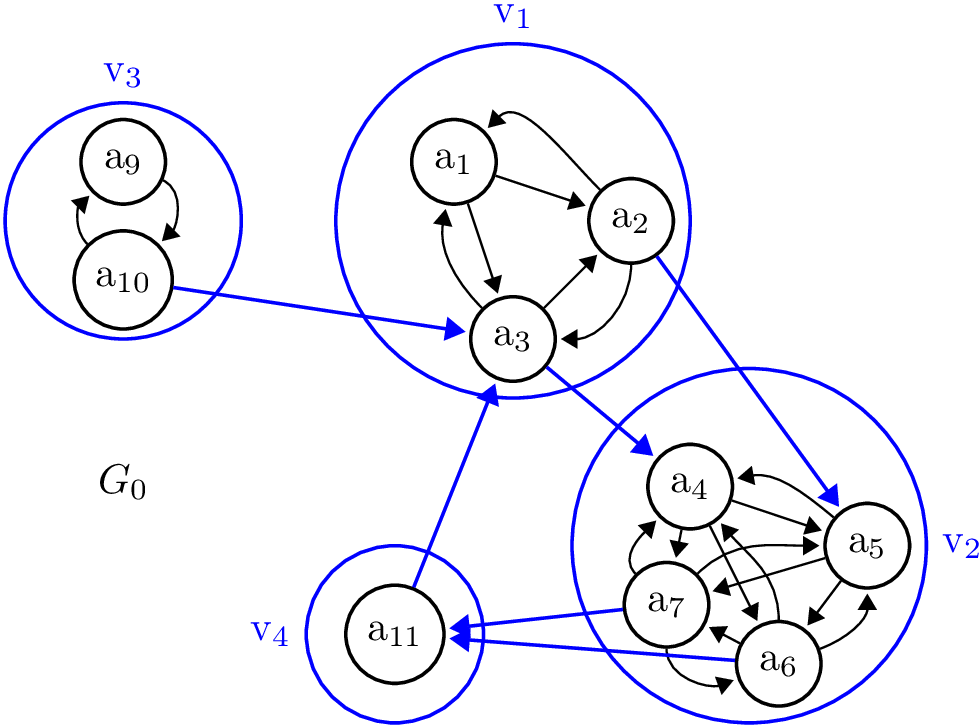
\includegraphics[scale=0.315]{Immagini/graph0.png}
    };

    \node[canvas is zy plane at x=5,draw,fill=white] at (0,0) {
        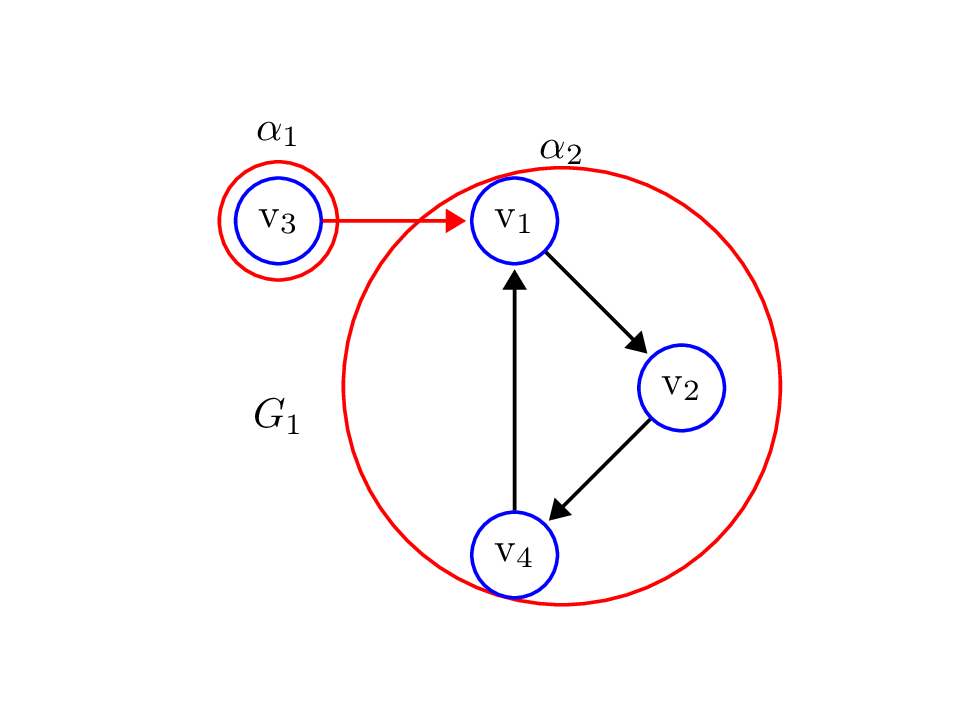
\includegraphics[scale=0.315]{Immagini/graph1.png}
    };

    \node[canvas is zy plane at x=10,draw,fill=white] at (0,0) {
        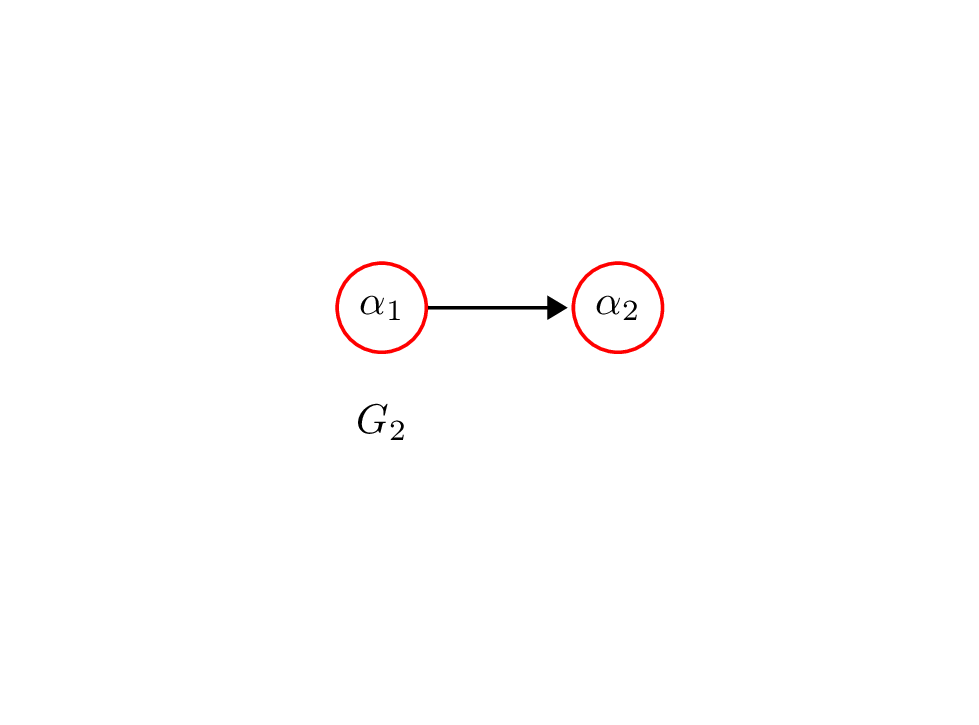
\includegraphics[scale=0.315]{Immagini/graph2.png}
    };
\end{tikzpicture}
    \caption{Esempio di grafo multi-livello}
    \label{fig:multi-level-graph-example}
\end{figure}

\newpage

\nlparagraph{Algoritmo di trasformazione naturale}\label{subsec:algoritmo-di-trasformazione-naturale}

La generica procedura algoritmica per realizzare la trasformazione naturale di un grafo standard $H = (W, F)$
preso in input in un grafo decontraibile $G = (V, E, dec_V, dec_E)$, può essere definita considerando la creazione di
supernodi e superarchi, costruendo implicitamente la funzione biiettiva $f_V: W \rightarrow V$ che realizza
l'isomorfismo tra i nodi di $H$ e i supernodi di $G$.

\begin{algorithm}[H] \floatname{algorithm}{Algoritmo}
    \begin{algorithmic}[1]
        \caption{NATURAL-TRANSFORMATION($H$)}\label{alg:natural-transformation}
        \State Sia $G = (V, E)$ un nuovo grafo decontraibile, con $V = \emptyset$ e $E = \emptyset$
        \For{$x \in W$}
            \State Sia $v$ un nuovo supernodo
            \State $v.dec \coloneqq (\emptyset, \emptyset)$
            \State $V \coloneqq V \cup \{v\}$
        \EndFor
        \For{$(x,y) \in F$}
            \State Sia $e$ un nuovo superarco
            \State $e.dec \coloneqq \emptyset$
            \State $E \coloneqq E \cup \{e\}$
        \EndFor
        \State \Return $G$
    \end{algorithmic}
\end{algorithm}

Tramite l'ausilio di strutture dati con tempi di ricerca costanti, come insiemi di hash, la complessit\`a delle
operazioni all'interno dei due cicli \`e $O(1)$,
e, di conseguenza, la complessit\`a dell'algoritmo \`e dettata dal numero di nodi e archi del grafo in input $H$,
ovvero $\mathbf{\Theta(|W| + |F|)}$.
\section{Procedure di Contrazione}\label{cap:procedure-contrazione}

In questa sezione si entrerà nel merito delle dinamiche interne alla costruzione della struttura di un grafo
multi-livello e alle sue funzioni di contrazione.
Sebbene nella Sezione~\ref{sec:algoritmi-di-enumerazione} siano già stati illustrati gli
algoritmi specifici per il riconoscimento e l'elencazione di pattern strutturali all'interno di un grafo,
nulla è stato ancora detto di come queste procedure di enumerazione debbano essere sfruttate nel contesto più
complesso del grafo multi-livello.
In particolare, si vuole dare una visione più chiara di come sia algoritmicamente
possibile realizzare una rete di collegamenti tra supernodi su più livelli attenendosi alle definizioni
fornite nella Sezione~\ref{sec:definizioni-e-proprieta-di-base} di questo capitolo, affinché si possa ottenere un tale
risultato a partire da una qualsiasi sequenza di insiemi di nodi generati dalle procedure di enumerazione,
evidenziandone complessità, problematiche e possibili soluzioni.

\subsection{Riduzione disgiunta}

Si vuole ora considerare il generico problema per cui, dato un grafo decontraibile $G = (V, E)$ e un insieme di
sottoinsiemi di nodi $Q \subseteq \mathcal{P}(V)$ che costituisce una copertura di $V$, si vuole costruire un grafo
decontraibile $G'$ che rappresenti l'informazione fornita dal raggruppamento dei nodi descritto in $Q$.
Aspetto di fondamentale importanza è che l'insieme $Q$ non costituisce necessariamente una partizione.
$Q$ potrebbe quindi essere calcolato a partire da un grafo $G$ attraverso un algoritmo di enumerazione, in modo tale
che i suoi elementi siano insiemi di nodi appartenenti ad un certo pattern strutturale.
Tuttavia, come si può immaginare, tali insiemi non sono necessariamente disgiunti: basti pensare alle cricche e i
circuiti semplici, che possono avere nodi in intersezioni di più insiemi.
Le componenti fortemente connesse invece, essendo costruite a partire da una relazione di equivalenza, sono un
valido esempio di pattern strutturale che costituisce sempre una partizione di $V$. \newline

D'ora in avanti, ci riferiremo agli elementi di una tale copertura di nodi $Q$ (non necessariamente disgiunta)
come \textbf{insiemi componenti} \newline

Per mantenere le proprietà delle contrazioni su grafi è però necessario che ad ogni nodo corrisponda ad uno ed un solo
supernodo.
La presenza dello stesso nodo in più supernodi contratti non sarebbe coerente con la teoria dei grafi
già affermata, oltre che portare ad un risultato che rischia di avere limitate applicabilità.
Si vuole quindi definire una procedura per rappresentare l'informazione fornita da $Q$ in un nuovo insieme che sia una
partizione di $V$ rappresentativa di $Q$ e, a partire da questa, costruire un grafo decontraibile $G'$.
Abbinare questa definzione generica, valida nella teoria degli insiemi, ad uno specifico algoritmo per calcolare
$Q$ a partire dalla struttura di un grafo, è il primo passo che permetterà di definire particolari funzioni di
contrazione.

\nlparagraph{Definzione}

\begin{definition}[Riduzione disgiunta]
Sia $V$ un insieme di elementi. Sia $Q \subseteq \mathcal{P}(V)$ una copertura di $V$.
Definiamo la \textbf{riduzione disgiunta} di $Q$, e la indichiamo con $\mathcal{D}(Q)$,
l'insieme di insiemi di elementi in $V$ tale per cui:
\begin{enumerate}[(i)]
    \item $\emptyset \notin \mathcal{D}(Q)$
    \item $\forall A \in \mathcal{D}(Q), \quad u, v \in A \Leftrightarrow \{C \in Q \mid u \in C\} = \{C \in Q \mid v \in C\}$
\end{enumerate}
\end{definition}

Una riduzione disgiunta di una copertura $Q$ è quindi un insieme di insiemi di nodi in $V$ tale per cui due
nodi $u$ e $v$ appartengono allo stesso insieme in $\mathcal{D}(Q)$ se e solo se sono inclusi nella stessa combinazione
di insiemi in $Q$. \newline

\begin{figure}[!h] \centering
\resizebox{!}{5.3cm}{
    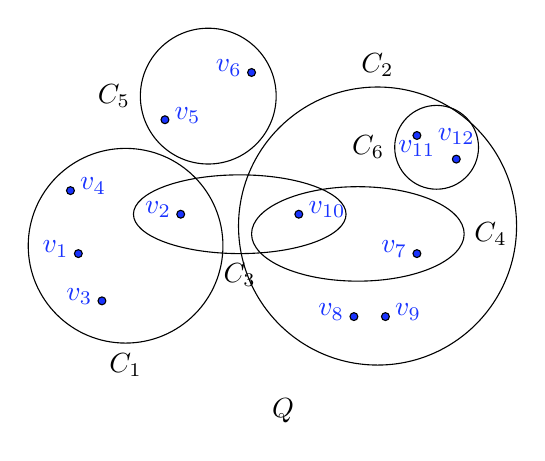
\begin{tikzpicture}[state/.style ={circle, draw, color=black , fill=blue, text=white, inner sep=0cm,
    minimum size=0.1cm}]
        \node[state] (1) [label={[left,text=blue]:$v_1$}] at (-0.3, 0) {};
        \node[state] (2) [label={[left,text=blue]:$v_2$}] at (1, 0.5) {};
        \node[state] (3) [label={[left,text=blue]:$v_3$}] at (0, -0.6) {};
        \node[state] (4) [label={[right,text=blue]:$v_4$}] at (-0.4, 0.8) {};
        \node[state] (5) [label={[right,text=blue]:$v_5$}] at (0.8, 1.7) {};
        \node[state] (6) [label={[left,text=blue]:$v_6$}] at (1.9, 2.3) {};
        \node[state] (7) [label={[left,text=blue]:$v_7$}] at (4, 0) {};
        \node[state] (8) [label={[left,text=blue]:$v_8$}] at (3.2, -0.8) {};
        \node[state] (9) [label={[right,text=blue]:$v_9$}] at (3.6, -0.8) {};
        \node[state] (10) [label={[right,text=blue]:$v_{10}$}] at (2.5, 0.5) {};
        \node[state] (11) [label={[below,text=blue]:$v_{11}$}] at (4, 1.5) {};
        \node[state] (12) [label={[above,text=blue]:$v_{12}$}] at (4.5, 1.2) {};

        \node[fit={(1)(2)(3)(4)}, draw, circle, label=below:$C_1$]{};
        \node[fit={(5)(6)}, draw, circle, label=left:$C_5$]{};
        \node[fit={(7)(10)},draw, ellipse, label=right:$C_4$, minimum width = 2.7cm]{};
        \node[fit={(2)(10)},draw, ellipse, label=below:$C_3$, minimum width = 2.7cm, minimum height = 1cm]{};
        \node[fit={(7)(8)(9)(10)(11)(12)}, draw, circle, label=above:$C_2$]{};
        \node[fit={(11)(12)}, draw, circle, label=left:$C_6$]{};
        \node (Q) at (2.3, -2) {$Q$};
    \end{tikzpicture}
    \hspace{0.5cm}
    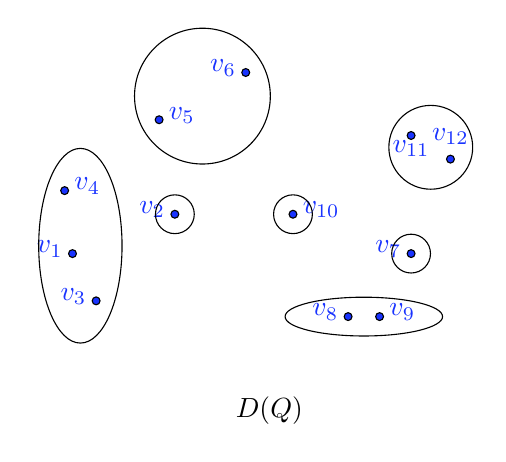
\begin{tikzpicture}[state/.style ={circle, draw, color=black , fill=blue, text=white, inner sep=0cm,
    minimum size=0.1cm}]
        \node[state] (1) [label={[left,text=blue]:$v_1$}] at (-0.3, 0) {};
        \node[state] (2) [label={[left,text=blue]:$v_2$}] at (1, 0.5) {};
        \node[state] (3) [label={[left,text=blue]:$v_3$}] at (0, -0.6) {};
        \node[state] (4) [label={[right,text=blue]:$v_4$}] at (-0.4, 0.8) {};
        \node[state] (5) [label={[right,text=blue]:$v_5$}] at (0.8, 1.7) {};
        \node[state] (6) [label={[left,text=blue]:$v_6$}] at (1.9, 2.3) {};
        \node[state] (7) [label={[left,text=blue]:$v_7$}] at (4, 0) {};
        \node[state] (8) [label={[left,text=blue]:$v_8$}] at (3.2, -0.8) {};
        \node[state] (9) [label={[right,text=blue]:$v_9$}] at (3.6, -0.8) {};
        \node[state] (10) [label={[right,text=blue]:$v_{10}$}] at (2.5, 0.5) {};
        \node[state] (11) [label={[below,text=blue]:$v_{11}$}] at (4, 1.5) {};
        \node[state] (12) [label={[above,text=blue]:$v_{12}$}] at (4.5, 1.2) {};

        \node[fit={(1)(3)(4)}, draw, ellipse]{};
        \node[fit={(5)(6)}, draw, circle]{};
        \node[fit={(2)}, draw, circle]{};
        \node[fit={(10)}, draw, circle]{};
        \node[fit={(7)}, draw, circle]{};
        \node[fit={(8)(9)}, draw, ellipse, minimum width = 2cm]{};
        \node[fit={(11)(12)}, draw, circle]{};
        \node (DQ) at (2.2, -2) {$D(Q)$};
    \end{tikzpicture}}
\caption{Esempio di riduzione disgiunta}
\label{fig:disjoint_reduction_example}
\end{figure}

L'esempio in Figura~\ref{fig:disjoint_reduction_example} fornisce una rappresentazione di una copertura $Q$ di
elementi (a sinistra) accompagnata dalla sua riduzione disgiunta $D(Q)$ (a destra).

Il nome di questa definizione deriva dal fatto che:
\begin{itemize}
    \item il risultato di questo operatore su una copertura $Q$, da solo non contiene le informazioni sufficienti a
        descrivere la copertura che lo ha originato, che potrebbero essere molteplici (ma non infinite, se si ha a che
        fare con insiemi finiti). %TODO: nota: potrebbe essere una classe di equivalenza tra coperture!!
        Da qui il termine \("\)riduzione\("\).
    \item il risultato di questo operatore su una copertura $Q$ di $V$ costituisce una partizione di $V$, come
        dimostrato in seguito, e fornisce un criterio per una suddivisione degli elementi in $V$ in insiemi disgiunti
        tra loro.
        Da qui il termine \("\)disgiunta\("\).
\end{itemize}

\begin{proposition}
Sia $V$ un insieme di elementi. Sia $Q \subseteq \mathcal{P}(V)$ una copertura di $V$.
La riduzione disgiunta di $Q$ costituisce una partizione di $V$.
\end{proposition}

\paragraph{Dimostrazione}
Si definisce la relazione $R_Q$ sull'insieme $V$ come
\begin{equation*}
    uR_{Q}v \Leftrightarrow \{C \in Q \mid u \in C\} = \{C \in Q \mid v \in C\}
\end{equation*}

Essa \`e una relazione di equivalenza, in quanto rispetta le propriet\`a di riflessivit\`a, simmetria e transitivit\`a,
che sono date dalle rispettive propriet\`a dell'uguaglianza.
Segue che l'insieme quoziente $V/R_{Q}$ deve rappresentare una partizione degli elementi in $V$.

Per il punto (ii) della definzione di $\mathcal{D}(Q)$, i suoi insiemi non vuoti rappresentano le classi di equivalenza
di $R_Q$.
Inoltre per il punto (i), l'insieme vuoto non pu\`o appartenere a $D(Q)$.
Si conclude allora $D(Q) = V/R_{Q}$, e pertanto $D(Q)$ \`e una partizione di $V$.

\nlparagraph{Definizione tramite ipergrafi}

Un \textit{ipergrafo} è una struttura simile ad un grafo non orientato dove ogni arco, detto \textit{iperarco},
anziché collegare una semplice coppia di nodi può connettere un arbitrario sottoinsieme di vertici.
Più formalmente, un ipergrafo $H$ è una coppia $(X, E)$ dove $X$ è un insieme di elementi chiamati nodi ed $E$ è
un insieme di sottoinsiemi di $X$ chiamati iperarchi.
Si consideri ora un ipergrafo non orientato $H = (X, E)$.
Notando che un iperarco non orientato $e \in E$ è a tutti gli effetti un insieme di nodi $e \subseteq V$,
si pu\`o estendere il concetto di rappresentazione disgiunta anche nel dominio degli ipergrafi.

\begin{definition}[Riduzione disgiunta di un ipergrafo]
    Dato un ipergrafo non orientato $H = (X, E)$ tale per cui $E$ \`e un ricoprimento di $X$,
    definiamo \textbf{riduzione disgiunta} di $H$ un nuovo ipergrafo non orientato $J = (W, F)$
    tale per cui $W = V$ e $F = \mathcal{D}(E)$.
\end{definition}

Si pu\`o notare, quindi, che la funzione di riduzione disgiunta pu\`o essere considerata come una
endofunzione idempotente sull'insieme degli ipergrafi non orientati.

\nlparagraph{Contrazione costruita da una partizione}

Motivo per cui la riduzione disgiunta di una copertura è certamente utile nel momento in cui si voglia
realizzare una funzione di contrazione, è che essa permette di ottenere una partizione di nodi.
La seguente ulteriore definizione permette di chiarire il passaggio che porta alla produzione in output di un grafo
decontraibile.

\begin{definition}[Contrazione costruita da una partizione]
Sia $G = (V, E)$ un grafo decontraibile, sia $P$ una partizione di $V$.
Si definisce \textbf{contrazione di $G$ costruita sulla partizione $P$} il grafo decontraibile
$G' = (\mathfrak{V}, \mathfrak{E})$ contrazione di $G$ tale per cui
    \begin{equation*}
        \{V_\alpha \mid \alpha \in \mathfrak{V}, dec_{\mathfrak{V}}(\alpha) = (V_\alpha, E_\alpha)\} = P
    \end{equation*}
\end{definition}

Dato un grafo decontraibile $G$ e una sua partizione dei nodi, quindi, è sempre possibile calcolare la sua
contrazione $G'$ contraendo nodi di $G$ in supernodi di $G'$ secondo gli insiemi descritti dalla partizione.
Si noti, infatti, che esiste una biiezione tra l'insieme delle possibili contrazioni di $G$ e l'insieme delle
partizioni di $V$ e che, pertanto, data una partizione di $V$ esiste una ed una sola contrazione di $G$ costruita
su di essa.

\nlparagraph{Algoritmo per la contrazione costruita da una riduzione disgiunta}\label{sec:make_decontractible_graph}

Entrambi i concetti esposti nel paragrafo precedente, ovvero la riduzione disgiunta di una copertura e la
contrazione costruita da una partizione, sono considerabili come elementi sufficientemente generici
per la definizione di una qualsiasi procedura di contrazione.
In particolare, il passaggio da una copertura
di nodi ad un grafo decontraibile può essere considerato come l'operazione successiva all'enumerazione degli
insiemi di nodi che costituiscono la copertura stessa. \newline

Risulta quindi utile definire un algoritmo che a partire da un grafo decontraibile $G$ e una sua copertura $Q$,
fornisca in output la contrazione di $G$ costruita sulla riduzione disgiunta di $Q$.

Una delle possibili rappresentazioni della copertura $Q$, da fornire in input a tale algoritmo, è quella un
\textit{dizionario} (talvolta anche detto ``mappa'' o ``tabella''), una struttura dati astratta che rappresenta una
collezione di coppie di elementi chiave-valore e le cui operazioni fondamentali consistono nell'inserimento e
cancellazione di coppie e ricerca di un valore mediante la sua chiave. \`E importante che in un dizionario
ad ogni chiave corrisponda al più un solo valore.
Negli pseudocodici, dato un dizionario $T$, l'operazione di ricerca di un valore associato ad una chiave $k$ verrà
indicata con $T[k]$, mentre l'operazione di inserimento di una coppia chiave-valore $(k, v)$ con $T[k] = v$.
Con $T.keys$ e $T.values$ si indicano rispettivamente l'insieme delle chiavi e l'insieme dei valori contenuti in $T$.

La copertura $Q$ è quindi data da un dizionario $T$ di dimensione $|V|$, in cui le coppie chiave-valore consistono di:
\begin{itemize}
    \item Chiave: nodo $v \in V$
    \item Valore: l'insieme di insiemi componenti $C \in Q$ tali per cui $v \in C$
\end{itemize}

Nel corso dell'algoritmo un altro dizionario $T'$ viene usato allo scopo di mappare la biiezione tra gli elementi
di $\mathcal{D}(Q)$ (quindi le classi di equivalenza di $V/R_Q$) e i supernodi di $G'$.
Aggiungendo coppie a $T'$, naturalmente al termine dell'algoritmo il dizionario $T'$ dovrà raggiungere la dimensione
$|\mathcal{D}(Q)|$. \newline

Nel ciclo a riga 3, si assegna ogni nodo del grafo decontaibile in input $G$ ad un supernodo, che esso sia
creato contestualmente o che sia il supernodo già creato corrispondente all'insieme di insiemi componenti in $v$.
Essendo che le precondizioni impongono che $T$ rappresenti una copertura di $V$, l'insieme $G.V$ a riga 3
potrebbe essere sostituito con $T.keys$.
Nel ciclo a riga 15, si assegnano gli archi di $G$ ai superarchi di $G'$. Se l'arco $(v, w)$ è interno ad un
supernodo, esso viene assegnato al suo insieme di archi. Se invece l'arco è tra collega due supernodi distinti, esso
viene assegnato al superarco corrispondente, che potrebbe essere contestualmente creato.

\begin{algorithm}[H] \floatname{algorithm}{Algoritmo}
    \caption{MAKE-DECONTRACTIBLE-GRAPH($T,G$)}\label{alg:make-decontractible-graph}
    \begin{algorithmic}[1]
        \State Sia $G' = (\mathfrak{V}, \mathfrak{E})$ un nuovo grafo decontraibile, con $\mathfrak{V} = \emptyset$
                e $\mathfrak{E} = \emptyset$
        \State Sia $T\mathcal{'}$ una nuova tabella, con insiemi di nodi come chiavi e supernodi come valori
        \For{$v\in G.V$}
            \If {$T[v]\notin T\mathcal{'}.keys$}
                \State Sia $\beta$ un nuovo supernodo con $G_{\beta}$ = $(\emptyset, \emptyset)$
                \State $\mathfrak{V}$ $\coloneqq$ $\mathfrak{V}$ $\cup$ $\{\beta\}$
                \State $T'[T[v]] \coloneqq \beta$
                \State $\alpha \coloneqq \beta$
            \Else
                \State $\alpha \coloneqq T'[T[v]]$
            \EndIf
            \State $V_{\alpha} \coloneqq V_{\alpha}$ $\cup$ $\{v\}$
            \State $v.supernode \coloneqq \alpha$
        \EndFor
        \For {$(v,w)$ in $G.E$}
            \State $\alpha \coloneqq v.supernode$
            \State $\beta \coloneqq w.supernode$
            \If {$(\alpha == \beta )$}
                \State $E_{\alpha} \coloneqq E_{\alpha} \cup \{(v,w)\}$
            \Else
                \If {$(\alpha , \beta)$ $\notin$ $\mathfrak{E}$}
                    \State $\mathfrak{E}$ $\coloneqq$ $\mathfrak{E}$ $\cup$ $\{(\alpha , \beta)\}$
                \EndIf
                \State $(\alpha , \beta).dec$ $\coloneqq$ $(\alpha , \beta).dec$ $\cup$ $\{(v, w)\}$
            \EndIf
        \EndFor
        \State \Return $G'$
    \end{algorithmic}
\end{algorithm}

In Figura~\ref{fig:make_decontractible_graph_example} sono rappresentati il grafo $G$, suddiviso in due insiemi
componenente e il corrispondente dizionario $T$ che ne rappresenta la copertura. Il dizionario $T\mathcal{'}$ \`e
rappresentato nello stato seguente all'applicazione dell'algoritmo MAKE-DECONTRACTIBLE-GRAPH con input $T$ e $G$,
contenendo come insieme di valori i supernodi ottenuti dalla contrazione di $G$.
Il risultato di MAKE-DECONTRACTIBLE-GRAPH($T$, $G$) \`e in questo caso il grafo decontraibile
$G'=(\{\alpha_1, \alpha_2, \alpha_3\}, \{(\alpha_1, \alpha_2), (\alpha_2, \alpha_3)\})$

\begin{figure}[H]
    \centering
    \begin{multicols}{3}
    \hspace{-1cm}
    \begin{tabularx}{0.8\linewidth} {
        | >{\raggedright\arraybackslash}X
        | >{\centering\arraybackslash}X | }
        \multicolumn{2}{>{\hsize=\dimexpr2\hsize+2\tabcolsep+\arrayrulewidth\relax}X}{\center$T$} \\
        \hline
        $v_1$ & $\{C_1\}$\\
        \hline
        $v_2$ & $\{C_1\}$\\
        \hline
        $v_3$ & $\{C_1, C_2\}$\\
        \hline
        $v_4$ & $\{C_2\}$\\
        \hline
        $v_5$ & $\{C_2\}$\\
        \hline
    \end{tabularx}
    \columnbreak \hspace{-1.75cm}
    \begin{tabularx}{0.8\linewidth} {
        | >{\raggedright\arraybackslash}X
        | >{\centering\arraybackslash}X | }
        \multicolumn{2}{>{\hsize=\dimexpr2\hsize+2\tabcolsep+\arrayrulewidth\relax}X}{\center$T'$} \\
        \hline
        $\{C_1\}$ & $\alpha_1$\\
        \hline
        $\{C_1, C_2\}$ & $\alpha_2$\\
        \hline
        $\{C_2\}$ & $\alpha_3$\\
        \hline
    \end{tabularx}
    \columnbreak \hspace{-1cm}
    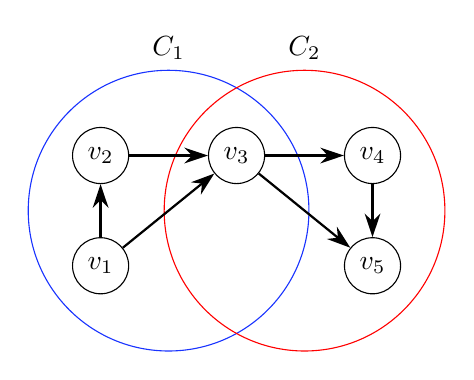
\begin{tikzpicture}

        \node[circle, draw] (A) {$v_1$};
        \node[circle, draw] (B) [above of=A, node distance=1.4cm] {$v_2$};
        \node[circle, draw] (C) [right=0cm and 1cm of B] {$v_3$};
        \node[circle, draw] (D) [right=0cm and 1cm of C] {$v_4$};
        \node[circle, draw] (E) [below of=D, node distance=1.4cm] {$v_5$};
        \begin{pgfonlayer}{background}
            \node[blue,
            circle,
            draw,
            fit=(A)(B)(C),
            label={[align=center, black]above:{$C_1$}}] (set1) {};
        \node[red,
            circle,
            draw,
            fit=(C)(D)(E),
            label={[align=center, black]above:{$C_2$}}] (set2) {};

        \end{pgfonlayer}
        \draw[myarrow] (A) -- (B);
        \draw[myarrow] (B) -- (C);
        \draw[myarrow] (A) -- (C);
        \draw[myarrow] (C) -- (D);
        \draw[myarrow] (D) -- (E);
        \draw[myarrow] (C) -- (E);
    \end{tikzpicture}
\end{multicols}
    \vspace{-30pt}
    \caption{Esempio di tabelle $T$ e $T'$ e del corrispondente grafo decontraibile}
    \label{fig:make_decontractible_graph_example}
\end{figure}

\paragraph{Complessità}
Facendo uso di tabelle di hash per rappresentare i dizionari $T$ e $T'$, l'algoritmo mantiene una complessit\`a
temporale di $O(|V| + |E|)$.
Si noti infatti che:
\begin{itemize}
    \item Il primo ciclo for scorre tutti i nodi in $V$.
    Esso inizializza il dizionario $T'$, definisce i supernodi di $G'$ e assegna loro i nodi in $V$.
    La complessità del ciclo è $O(|V|)$, infatti il controllo a riga 3 ha complessità costante,
    così come le ricerca in $T$ e $T'$ alle righe 7 e 10.
    \item Il secondo ciclo for scorre tutti gli archi in $E$.
    Esso assegna gli archi di $G$ ai grafi dei supernodi di $G'$ o ai superarchi di $G'$ a seconda dei supernodi
    di appartenenza dei nodi che li compongono, ottenibili in tempo $O(1)$ in quanto precedentemente calcolati nel
    primo ciclo for. La complessit\`a del ciclo \`e $O(|E|)$.
\end{itemize}

\subsection{Algoritmi di contrazione}\label{sec:algoritmi-di-contrazione}

In questa sezione illustriamo brevemente come a partire dagli algoritmi di enumerazione di sottoinsiemi descritti
e dall'algoritmo per la contrazione costruita da una rappresentazione disgiunta, \`e quindi possibile costruire
delle procedure complete che rappresentino delle funzioni di contrazione.

\nlparagraph{Procedure per la gestione dei dizionari}\label{subsec:procedure-per-la-gestione-deli-dizionari}

Come si pu\`o notare dallo pseudo-codice dagli algoritmi di enumerazione descritti nel
Capitolo~\ref{ch:algoritmi-di-enumerazione}, ciascuno di essi provvede a fornire in output una sequenza di
sottoinsiemi di nodi che rispettino il pattern strutturale individuato.
Allo scopo di costruire una funzione di contrazione, \`e però necessario che tali insiemi siano usati per definire
una copertura di nodi rappresentata attraverso un dizionario $T$, come descritto nella sezione precedente.
Per questo motivo si propongono una serie di procedure che permettano di inizializzare, aggiungere e rimuovere
sottoinsiemi da un dizionario $T$, affinché queste possano essere usate come integrazione per fornire un
adattamento dello pseudo-codice originale degli algoritmi di enumerazione presentati. \newline

In particolare, come riga iniziale di ciascuno di questi algoritmi, può essere aggiunta la seguente procedura per
l'inizializzazione del dizionario $T$.

\begin{algorithm}[H]
    \caption{INITIALIZE-TABLE($V$)}\label{alg:init-table}
    \begin{algorithmic}[1]
        \State Let $T$ be a new table
        \For{$v \in V$}
            \State $T[v] \coloneqq \emptyset$
        \EndFor
        \State return $T$
    \end{algorithmic}
\end{algorithm}

L'operazione di fornire in output un insieme componente potrebbe essere invece sostituita in ciascun algoritmo
con la seguente procedura per l'aggiunta di un insieme $C$ all'insieme di insiemi componente tracciati da $T$. \newline

\begin{algorithm}[H] \floatname{algorithm}{Algoritmo}
    \caption{ADD-COMPONENT-SET($T$, $C$)}\label{alg:add-subset}
    \begin{algorithmic}[1]
        \For{$v\in C$}
            \State $T[v]:=T[v] \cup \{C\}$
            \State $T.modified:=T.modified \cup \{v\}$
        \EndFor
    \end{algorithmic}
\end{algorithm}

Per completezza si fornisce anche la procedura per la rimozione di un insieme $C$ da $T$.

\begin{algorithm}[H]
    \caption{REMOVE-SUBSET($T$, $C$)}\label{alg:rem-subset}
    \begin{algorithmic}[1]
        \For{$v\in C$}
            \State $T[v]:=T[v] \setminus \{C\}$
            \State $T.modified:=T.modified \cup \{v\}$
        \EndFor
    \end{algorithmic}
\end{algorithm}

Nel caso in cui si avesse a che fare con procedure di enumerazione che forniscono in output insiemi di nodi che non
necessariamente forniscono una copertura di tutti i nodi del grafo (come nel caso dell'algoritmo di enumerazione
dei circuiti semplici), la seguente procedure può essere utilizzata al termine dell'enumerazione per aggiungere
ciascun nodo rimasto escluso dalla copertura a un insieme componente singoletto. Come evidente dallo
pseudocodice, tale procedura manterrebbe una complessit\`a temporale di $O(|V|)$, con |V| il numero di nodi del grafo
decontraibile da contrarre.

\begin{algorithm}[H] \floatname{algorithm}{Algoritmo}
    \caption{ADD-SINGLETONS($T$)}\label{alg:add-singletons}
    \begin{algorithmic}[1]
        \For{$v \in T.keys$}
            \If{$T[v] == \emptyset$}
                \State $T[v] := \{v\}$
            \EndIf
        \EndFor
    \end{algorithmic}
\end{algorithm}

Si pu\`o notare che le procedure di aggiunta e rimozione di un sottoinsieme $C$ da $T$ prevedono il tracciamento
dei particolari nodi corrispondenti a record di $T$ modificati, attraverso l'utilizzo di un insieme associato
alla tabella e indicato come $T_{modified}$.
Sebbene non sia necessario per le procedure di contrazione, questo risulterà utile per rendere le procedure
applicabili anche nelle procedure di aggiornamento dinamico al grafo contratto, come verrà trattato nel capitolo~\ref{}.
L'insieme $T_{modified}$ permetterà, infatti, di evitare di scorrere l'intero dizionario $T$ nel momento in cui il
grafo contratto già costruito dovrà essere aggiornato in accordo alle modifiche agli insiemi componente tracciati
da $T$. \newline

\nlparagraph{Aggiunta di un sottoinsieme massimale}

Sebbene alcuni algoritmi di enumerazione possano già fornire in output sottoinsiemi di nodi tra loro massimali,
come nel caso dell'algoritmo di enumerazione delle componenti fortemente connesse e delle cricche massimali,
in generale non è garantito che ciò avvenga, come nel caso dell'algoritmo di enumerazione dei circuiti semplici.
Qualora sia necessario adattare una funzione di contrazione affinché questa sia basata sui soli insiemi di nodi
massimali forniti da un algoritmo di enumerazione, la procedura descritta di seguito può essere utilizzata in
sostituzione della normale procedura ADD-COMPONENT-SET.
Infatti, questa procedura permette controllare contestualmente alla sua aggiunta a $T$ se un dato sottoinsieme $C$ di
nodi sia massimale rispetto agli altri insiemi già tracciati in $T$ e, se si, individuare quali eventuali sottoinsiemi
in $T$ siano inclusi in $C$, affinché possano essere rimossi.

\begin{algorithm}[H]
    \caption{ADD-MAXIMAL-SUBSET($T$, $C$)}\label{alg:add-maximal-subset}
    \begin{algorithmic}[1]
        \If{$\bigcap_{v \in C}T[v] == \emptyset$}
            \State $Q :=$ FIND-SUBSETS($T$, $C$)
            \For {$S \in Q$}
                \State REMOVE-SUBSET($T$, $S$)
            \EndFor
            \State ADD-SUBSET($T$, $C$)
        \EndIf
    \end{algorithmic}
\end{algorithm}
\begin{algorithm}[H] \floatname{algorithm}{Algoritmo}
    \caption{FIND-SUBSETS($T$, $C$)}\label{alg:find-subsets}
    \begin{algorithmic}[1]
        \State Sia $T_c$ una nuova tabella per contare le occorrenze dei sottoinsiemi
        \For{$v \in C$}
            \For{$S \in T[v]$}
                \State $T_c[S] := T_c[S] + 1$
            \EndFor
        \EndFor
        \State $Q := \emptyset$
        \For {$S \in T_c$}
            \If{$T_c[S] == |C|$}
                \State $Q := Q \cup \{S\}$
            \EndIf
        \EndFor
        \State \Return $Q$
    \end{algorithmic}
\end{algorithm}

In particolare, l'algoritmo ADD-MAXIMAL-COMPONENT-SET provvede innanzitutto a verificare a riga 1 che l'insieme $C$ non
sia gi\`a incluso in un altro insieme presente tra gli insiemi di $T$, ovvero che non sia certamente
massimale.
Questo viene verificato controllando se tutti i nodi in $C$ condividano l'appartenenza ad uno o pi\`u insiemi gi\`a
presenti. \newline
Se l'insieme $C$ \`e massimale rispetto ai nodi trovati, succesivamente l'algoritmo provvede ad individuare
gli eventuali insiemi presenti in $T$ che siano sottoinsiemi di $C$ attraverso la procedura FIND-SUBSETS.
Essa conteggia il numero di volte che ciascun sottoinsieme appare tra i nodi di $C$ rispetto al dizionario $T$.
Un conteggio pari alla cardinalit\`a dell'insieme stesso testimonia che tutti i suoi nodi sono presenti in $C$.

\paragraph{Complessit\`a}
Con l'utilizzo di insiemi basati su hash, in cui la complessit\`a per verificare l'appartenenza ad un insieme \`e
$O(1)$, la complessit\`a della procedura di ADD-MAXIMAL-SUBSET risulta essere $O(|C| \cdot c_{max})$ nel caso peggiore,
dove $|C|$ \`e la cardinalit\`a dell'insieme $C$ in input e $c_{max}$ \`e l'upper bound del numero di sottoinsiemi
massimali già tracciati dalla tabella $T$, che risulta essere massimo quando la cardinalit\`a di questi insiemi
\`e pari alla met\`a del numero di nodi del grafo $G = (V, E)$ che si sta contraendo.
Si noti che la complessit\`a apportata da $c_{max}$ non pu\`o mai essere
superiore all' esponenziale, in quanto, in generale, il numero massimo di insiemi massimali che possono essere
individuati in un insieme di $n$ elementi rimarr\`a sempre inferiore al numero di tutti i possibili sottoinsiemi,
che è $2^n$.
Sebbene il termine $c_{max}$ possa essere considerato come un $O(2^n)$ nel calcolo della complessit\`a (con $n = |V|$
il numero di nodi del grafo), esso pu\`o essere calcolato in modo pi\`u preciso come segue:

\begin{equation*}
    c_{max} \quad = \quad \binom{n}{\lfloor \frac{n}{2} \rfloor} = \frac{n\cdot(n-1)\cdot\ldots\cdot(n/2)}{\frac{n}{2}!}
\end{equation*}

La complessit\`a della procedura pu\`o essere calcolata notando che l'intersezione nel controllo a riga 1 pu\`o
impiegare al pi\`u $O((|C|-1) \cdot max_{v \in C}\{|T[v]|\})$.
Tuttavia, eseguendo le intersezioni a partire dall'insieme $T[v]$ pi\`u piccolo, individuato in tempo lineare a
$|C|$, la complessit\`a pu\`o essere ridotta a $O((|C|-1) \cdot min_{v \in C}\{|T[v]|\})$.
In ogni caso, questa complessit\`a pu\`o essere riscritta come $O(|C| \cdot c_{max})$, considerando il caso peggiore
in cui tutti i nodi in $C$ appartengono agli insiemi costruiti tramite unione tra i possibili sottoinsiemi massimali
tra i restanti $|V|-|C|$ nodi del grafo e $C$, tutti di egual cardinalit\`a.
Inoltre la procedura FIND-SUBSETS impiega anch'essa al pi\`u $O(|C| \cdot c_{max})$ tempo,
in quanto il ciclo for a riga 2 scorre tutti i nodi in $C$, mentre il ciclo for a riga 3 scorre tutti i
sottoinsiemi massimali presenti in $T$ per ogni nodo in $C$, che sono al pi\`u pari a tutti i sottoinsiemi massmali
ottenibili a partire dai restanti $|V|-1$ nodi del grafo.
Inoltre il ciclo for a riga 8 scorre tutti i sottoinsiemi massimali trovati, che sono al pi\`u pari a $c_{max} - 1$,
considerato che l'insieme $C$ deve essere anch'esso massimale.

\nlparagraph{Procedure complete di contrazione}

Forniamo ora una descrizione della struttura di un algoritmo generico che rappresenti la procedura completa di
contrazione di un grafo decontraibile $G$, ovvero che permetta di realizzare una funzione di contrazione $f_C$
che possa essere usata nella definzione di un grafo multilivello.

Esso pu\`o essere costituito dalle seguenti fasi:
\begin{enumerate}
    \item Fase di pre-elaborazione (opzionale) \\
    Dato il grafo iniziale $G$, si produce un nuovo grafo $H$ adatto ad essere fornito in input all'algoritmo
    della fase successiva.
    Questo potrebbe essere utile allo scopo di adattare il grafo all'algoritmo, migliorare le performance o
    costruire un nuovo grafo che rappresenti particolari relazioni tra i nodi del grafo originale oltre alla
    semplice adiacienza.
    \item Fase di enumerazione dei sottoinsiemi \\
    Nel grafo $H$ vengono riconosciuti i pattern strutturali dallo specifico algoritmo di enumerazione e tracciati
    sotto forma di insiemi componenti composti dai nodi che fanno parte di tali pattern.
    Il riultato \`e la mappatura $T$ tra i nodi del grafo $H$ e l'insieme dei sottoinsiemi di cui fanno parte.
    \item Fase di contrazione \\
    Viene restituita la contrazione di $G$ costruita sulla rappresentazione digiunta dei sottoinsimi individuati,
    secondo la logica dell'algoritmo MAKE-CONTRACTIBLE-GRAPH\@.
\end{enumerate}

\begin{algorithm}[H]
    \caption{GENERIC-CONTRACTION($G$)}\label{alg:generic-contraction}
    \begin{algorithmic}[1]
        \State Let $H$ be a graph obtained from $G$ by a preprocessing procedure
        \State Let $T$ be a table obtained from $H$ by a generic subset enumerating algorithm
        \State $J$ = MAKE-CONTRACTIBLE-GRAPH($T$, $G$)
        \State return $J$
    \end{algorithmic}
\end{algorithm}

Gli algoritmi di contrazione relativi ai problemi di enumerazione trattati potrebbero seguire la struttura sopra
descritta nei seguenti modi:
\begin{itemize}
    \item Per la contrazione per componenti fortemente connesse la fase di preprocessing potrebbe essere
    essere saltata, in quanto l'algoritmo di Kosaraju-Sharir e la sua versione adattata non necessitano di alcuna
    modifica al grafo orientato in input.
    \item Per la contrazione per cricche può essere utilizzata una fase di preprocessing per la costruzione
    della relativa versione non orientata di un grafo, che potrebbe sostituire tutti gli archi orientati con
    archi non orientati, oppure che potrebbe mantenere un arco non orientato solo per quelle coppie di nodi
    mutualmente adiacenti.
    La fase di enumerazione può essere realizzata dalla versione adattata dell'algoritmo di Bron-Kerbosch.
    \item Per la contrazione per circuiti semplici pu\`o essere utilizzata una fase di preprocessing per
    l'eliminazione di tutti gli archi tra nodi che non facciano parte delle stesse componenti fortemente connesse
    allo scopo di migliorare le performance della fase di enumerazone che può essere realizzata dall'algoritmo
    di Johnson nella sua versione adattata.
\end{itemize}







\chapter{Applicazione dei Grafi Multilivello ai Sogni} \label{cap:applicazione-dei-grafi-multilivello-ai-sogni}

Come testimoniato dalle loro svariate applicazioni, nella loro generalità e semplicità, i grafi si sono da sempre
dimostrati strutture in grado di catturare l'essenza di tanti aspetti della realtà dalla più variegata natura.
Che siano reti sociali, reti di trasporto, reti di comunicazione, reti biologiche, reti semantiche o reti di calcolo,
essi permettono di fornire un utile modello per la rappresentazione di dati complessi.
Il fatto che i grafi multi-livello siano proprio basati su grafi conferisce loro una notevole versatilità che permette
di applicarli ad una vasta gamma di problemi, tra cui l'analisi di testi in linguaggio naturale,
ed in particolare, a racconti di sogni.
Tuttavia il potenziale dei grafi multi-livello, che si basa sulla loro capacità di catturare aspetti della struttura
di un grafo ad un livello di astrazione superiore, è ciò che li rende particolarmente interessanti e che può
fornire un valore aggiunto all'analisi delle relazioni di elementi discreti, come le parole di un testo. \newline

Si noti, infatti, che nel contesto generale dell'analisi di grafi, la contrazione realizzata attraverso
l'uso di grafi multi-livello potrebbe essere utile per:
\begin{itemize}
    \item Ridurre la complessit\`a dell'analisi strutturale di un grafo, sia che esso debba essere processato
    attraverso algoritmi costosi, sia che esso debba essere graficamente visualizzato, rendendolo pi\`u facilmente
    interpretabile ed evidenziandone le caratteristiche strutturali di interesse.
    \item Studiare l'interrelazione di caratteristiche strutturali di un grafo, che rappresenti la navigabilit\`a
    di uno spazio basato su componenti fortemente connesse, cicli, cricche ecc.
    Si noti che gli spazi generati da livelli superiori al primo non potrebbero essere altrimenti ottenuti se
    non attraverso un approccio multi-livello.
    \item Stabilire il grado di connettivit\`a di un grafo, individuando la rilevanza (intesa come il numero di
    insiemi componente che rappresentano i supernodi), il numero e la dimensione delle sue contrazioni.
    \item Misurare il grado di complessit\`a dello spazio rappresentativo del grafo, in base al numero
    di nodi e archi presenti nelle contrazioni: grafi derivanti da specifici domini tendono ad avere un certo
    grado di complessit\`a legato ad un concetto spaziale, come successivamente mostrato nell'
    esempio~\ref{fig:les-miserables-graph}.
    \item Valutare l'influenza di singoli nodi e archi appartenenti al grafo di base sui livelli superiori
    del grafo multi-livello, eseguendo analisi della sensitivit\`a e della robustezza.
    Sebbene non siano presentate in questa tesi, è possibile definire delle procedure che permettano di aggiornare
    coerentemente la struttura memorizzata di un grafo multi-livello all'aggiunta e rimozione di singoli nodi e
    archi al livello base.
\end{itemize}

Nel contesto dell'analisi di testi, in particolare di racconti di sogni, con l'eventuale ausilio di strumenti di
elaborazione del linguaggio naturale, la contrazione realizzata attraverso l'uso di grafi multi-livello potrebbe
essere utile per:
\begin{itemize}
    \item Individuare contesti sintattici e possibilmente semantici di parole nel contesto del mondo onirico
    di un particolare sognatore, evidenziando l'interrelazione e la distanza tra gruppi di parole e frasi.
    \item Valutare la somiglianza sintattica di singoli racconti, individuando le macro-caratteristiche
    strutturali comuni tra i sogni di singoli individui e usarle per differenziare e catalogare più sognatori.
    \item Individuare pattern ricorrenti di parole e insiemi di parole su un corpus ampio di testi, con
    eventuale ausilio di strumenti statistici
    \item Stabilire la natura della connettività del grafo delle parole in base al numero di insiemi componente
    (gruppi di parole) e di nodi presenti nelle contrazioni.
    \item Permettere un confronto automatico dei pattern strutturali con grafi multi-livello che rappresentino
    un controllo, con l'eventuale ausilio di algoritmi che valutano il grado di somiglianza di grafi.
\end{itemize}

In questo capitolo verranno, quindi, esplorate le possibili modalità di applicazione dei grafi multi-livello allo scopo
di analisi di racconti di sogni, portando dei casi di studio reali, con l'obiettivo di evidenziarne le capacità
nell'ambito di un'analisi sintattica e semantica.
Tutti i sogni utilizzati nelle analisi sono stati prelevati da DreamBank.net \footnote{DreamBank.net, \url{https://dreambank.net/}}
un dataset di sogni provenienti da diverse fonti e studi di ricerca, disponibile liberamente online, mentre le
immagini di grafi sono state realizzate attraverso il software open-source Gephi \footnote{Gephi, https://gephi.org/}
abbinato all'uso del plugin MultiViz~\cite{s2022multivizgephipluginscalable} per la visualizzazione a più livelli.

\section{Analisi dei contesti semantici di un sognatore}\label{sec:analisi-dei-contesti-semantici-di-un-sognatore}

L'estrapolazione di informazioni legate al significato delle parole a partire da aspetti sintattici \`e un
principio fondamentale della semantica computazionale, noto come \textit{ipotesi distribuzionale}, che si basa sul
principio per cui il significato di una parola \`e determinato dal suo contesto di utilizzo, e che le parole che
appaiono nello stesso contesto tendono ad avere significati simili.\newline
In questa sezione verrà esplorato un caso di studio, risultato del tentativo di usare il modello dei grafi multi-livello
allo scopo di individuare dei contesti di parole di valenza sintattica e semantica all'interno del mondo onirico
di una particolare sognatrice.
Daremo forma allo spazio delle parole di Emma a partire da un vasto corpus di racconti di sogni, e analizzeremo la
struttura del grafo multi-livello risultante.

\subsection{Fase di pre-elaborazione}

Per poter procedere con l'analisi dei sogni di Emma affinché si potesse costruire un grafo delle parole
da cui poter cogliere aspetti semantici, si è ritenuto necessario aggiungere dei passaggi ulteriori
al processo di pre-elaborazione descritto nella sottosezione~\ref{subec:pre-elaborazione-con-NLP}.
In particolare, si è rivelato utile allo scopo di un'analisi semantica,
un filtraggio delle parole meno frequenti rispetto all'intero corpus di sogni di Emma.
Questo passaggio è stato eseguito per ridurre la complessità del testo e concentrare l'analisi sui
termini più rilevanti e significativi, con l'obiettivo di individuare le tematiche principali trattate
nei sogni e l'ordine con cui esse appaiono nei testi.
Un'altra possibile interessante fase di pre-elaborazione ulteriore è quella dell'estrapolazione di categorie
specifiche di parole.
Attraverso tecniche di NLP come il Part-of-Speech (POS) tagging, ciascuna parola può essere etichettata con la sua
categoria grammaticale di appartenenza, come quella dei sostantivi, verbi, aggettivi, avverbi, ecc.
Con la tecnica di Named Entity Recognition (NER) tagging è possibile, invece, identificare le entità di interesse
all'interno del testo, categorizzando elementi come persone, luoghi e organizzazioni.
A partire da queste categorizzazioni, tutte le parole che non sono etichettate in una particolare
categoria vengono filtrate. Lo scopo di questa fase potrebbe essere quello di concentrare l'analisi sulle parole che
sono considerate le parti del testo più significative e ricche di contenuto, o semplicemente focalizzare l'analisi
su un aspetto di interesse.


\nlparagraph{Connettività del grafo delle parole}

Sebbene il grafo delle parole risultante dalla pre-elaborazione di tutti i sogni di un particolare sognatore
sia frutto di un processo di semplificazione e riduzione della complessità del testo, la sua analisi diretta
attraverso l'uso del grafo multi-livello ne ha rivelato sin da subito la sua elevata connettività derivante dalla
natura del linguaggio naturale: parole e concetti possono essere strettamente legati (e quindi ``vicini'') ad un
ampio numero di altri concetti che a loro volta possono collegarsi direttamente ad altri concetti sparsi per il grafo.
Il risultato è uno spazio fortemente ``aggrovigliato'' che non favorisce la formazione di gruppi di parole distinti e
ben definiti e che, di conseguenza, non favorisce un processo di contrazione di qualità nella
gerarchia del grafo multi-livello.

Per rendere chiaro questo aspetto, si prenda come esempio il grafo multi-livello $M = (G, \langle f_{C_1}, f_{C_2}\rangle)$
rappresentato in figura~\ref{fig:les-miserables-graph}, il cui grafo $G$ rappresenta il grafo delle relazioni di
co-apparizione dei personaggi del romanzo \textit{Les Misérables} di Victor Hugo,
e le cui funzioni di contrazione $f_{C_1}$ e $f_{C_2}$ rappresentano rispettivamente le funzioni di contrazione
per cricche non reciproche e stelle.
Appare evidente di come la struttura del grafo $G$ sia stata contratta con un elevato tasso di contrazione,
producendo una struttura notevolmente più semplice e facilmente interpretabile. Per via degli schemi di
contrazione scelti, appare evidente come la struttura originale del grafo abbia rivelato la sua ordinatezza ai livelli
superiori: in media i personaggi del romanzo possono apparire assieme ad una cerchia ristretta di altri personaggi,
ad eccezione di personaggi principali che risultano collegarsi a questi gruppi più o meno isolati di nodi.
Questo rispecchia in parte la natura dello spazio bidimensionale in cui i personaggi sono collocati: personaggi
appartenenti a luoghi distanti difficilmente appariranno insieme. I personaggi principali, in quanto seguiti
nella narrazione nel mentre che si spostano nello spazio, permettono di rompere questa dimensionalità, e risultano
essere collegati a nodi distanti tra loro.

\begin{figure}[h]
    \centering
    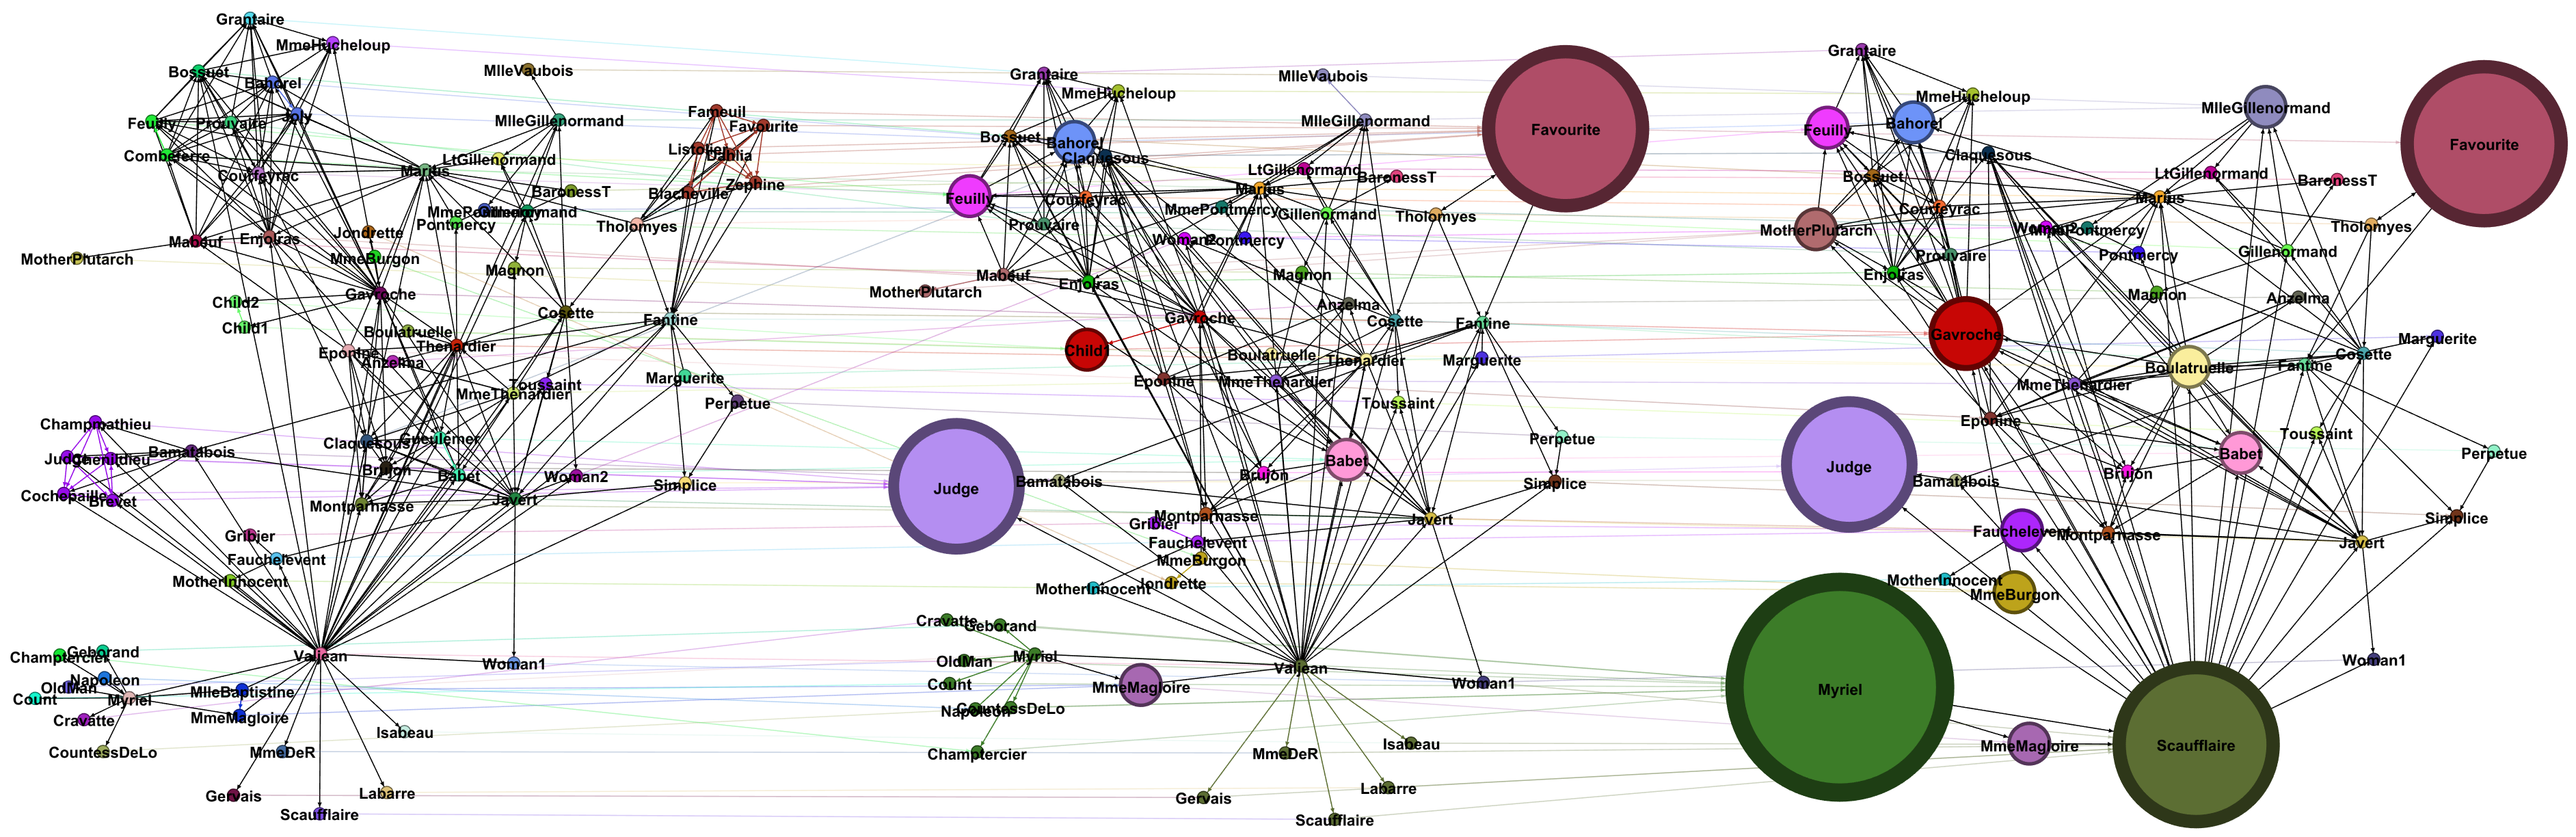
\includegraphics[width=1\textwidth]{Immagini/les_miserables_example}
    \caption{Grafo multi-livello delle co-apparizioni in \textit{Les Misérables}}
    \label{fig:les-miserables-graph}
\end{figure}

Per risolvere questo problema legato all'alta connettività del grafo delle parole, si è deciso di applicare
una tecnica di potatura del grafo, che consiste nell'identificazione di uno scheletro portante del grafo
basato sulle relazioni più significative tra le parole e dell'esclusione delle relazioni meno significative in
accordo a tale scheletro, allo scopo di ``appiattire'' lo spazio delle parole.

\nlparagraph{Classificazione degli archi}

L'algoritmo di potatura del grafo si basa sulla rilevanza delle relazioni tra le parole, ovvero degli archi del grafo.
Sebbene la rilevanza di un bigramma possa essere definita e valutata in diversi modi - come ad esempio il calcolo
dell'informazione mutua puntuale (PMI) tra le parole - in questo caso si è scelto di basare la rilevanza
direttamente sull'informazione fornita dai pesi degli archi e dei relativi nodi coinvolti.
In particolare, la misura di rilevanza di un arco è stata definita come la somma dei rapporti tra il peso dell'arco
e i singoli pesi dei nodi su cui l'arco è incidente.
In formule, siano $w(u)$, $w(v)$ e $w(u, v)$ il peso del nodo $u$ e $v$ e dell'arco $(u, v)$ rispettivamente,
la rilevanza dell'arco $(u, v)$ è definita come:
\begin{equation*}
    relevance(u, v) = \frac{w(u, v)}{w(u)} + \frac{w(u, v)}{w(v)}
\end{equation*}

La formula fornisce un criterio elementare per distinguere la frequenza di coppie di parole dalla loro importanza:
un arco con un peso elevato rispetto ai pesi dei nodi coinvolti è considerato più rilevante di un arco con un peso
elevato rispetto alla media dei pesi degli altri archi.
Ad esempio, un arco con peso 10 tra due nodi con pesi 100 e 200 è considerato meno rilevante di un arco con peso 5
tra due nodi con pesi 8 e 10. \newline

La scelta di questa misura di rilevanza è dovuta alla facilità con cui è possibile associarla ad un nuovo valore
positivo che rappresenti una distanza semantica tra le parole collegate.
Essendo tale valore di rilevanza sempre compreso nell'intervallo $(0, 2]$, è possibile definire un valore di costo
semantico dell'arco $(u, v)$ come $\frac{1}{relevance(u, v)}$, che è inversamente proporzionale alla
rilevanza dell'arco.
Gli archi possono, quindi, essere classificati in base a questo valore di distanza che d'ora in avanti chiameremo
\textit{costo} dell'arco.

\nlparagraph{Algoritmo per la riduzione della connettività}

Un algoritmo che sfrutti l'informazione data dal costo degli archi per ridurre la complessità e la connettività
di un grafo potrebbe agire costruendo in maniera incrementale un nuovo grafo a partire da quello fornito in input,
che ne rappresenti una versione semplificata.
L'algoritmo proposto nel seguente pseudocodice considera gli archi del grafo in input $G$ in ordine crescente di
costo al fine di valutarne l'inclusione nel nuovo grafo semplificato $H$, sulla base di un ulteriore parametro in input
che chiamiamo \textit{threshold}.

In particolare, ogni nodo del grafo originale $G$ sarà presente nel grafo semplificato $H$. Mentre per ogni arco $(u, v)$
di $G$ considerato nel ciclo for a riga 4, se nella versione non orientata di $H$, ottenuta rimuovendo l'orientamento
degli archi, esiste già un cammino tra i nodi $u$ e $v$ e il costo del cammino minimo calcolato sul costo degli archi
è maggiore al threshold, l'arco $(u, v)$ viene ignorato, altrimenti viene aggiunto al grafo semplificato $H$.
Si noti che nello pseudocodice, così come nella notazione tipica, un costo di cammino minimo pari a $\infty$ indica
che non esiste un cammino tra i nodi.

\begin{algorithm}[H]
    \caption{REDUCE-CONNECTIVITY($G$, $threshold$)}\label{alg:reduce-connectivity}
    \begin{algorithmic}[1]
        \State Sia $H = (W, F)$ un nuovo grafo orientato, con $W = G.V$ e $F = \emptyset$
        \State Sia $H_u = (W_u, F_u)$ un nuovo grafo non orientato, con $W_u = G.V$ e $F_u = \emptyset$
        \State Ordina gli archi in $G.E$ in ordine crescente di costo
        \For {$(u, v) \in G.E$}
            \State Sia $d$ il costo del cammino minimo tra $u$ e $v$ in $H_u$ calcolato sulla base del costo degli archi
            \If{$d == \infty$ \textbf{or} $d < threshold$}
                \State $F = F \cup \{(u, v)\}$
                \State $F_u = F_u \cup \{\{u, v\}\}$ \Comment{L'arco aggiunto ha lo stesso costo di $(u, v)$}
            \EndIf
        \EndFor
        \State \textbf{return} $H$
    \end{algorithmic}
\end{algorithm}

In questo modo, l'algoritmo costruisce arco dopo arco un grafo semplificato $H$ basato sui collegamenti più
rilevanti tra le parole.
Gli archi che vengono ignorati sono quelli che collegano parole considerate distanti secondo i collegamenti più
rilevanti stabiliti nello scheletro provvisorio del grafo $H$.
Il grado di tolleranza alla distanza tra le parole è regolato dal parametro \textit{threshold},
che può essere impostato per ottenere un grafo più o meno semplificato: più basso sarà il threshold, minore
sarà il grado di connettività del grafo prodotto.

\paragraph{Complessità}
Il costo dell'algoritmo REDUCE-CONNECTIVITY è principalmente dominato dalla fase di ordinamento degli archi
e del calcolo dei cammini minimi tra i nodi del grafo non orientato $H_u$.
Utilizzando algoritmi di ordinamento efficienti, il costo computazionale dell'ordinamento a riga 3 è $O(|E| \log |E|)$.
Il calcolo dei cammini minimi tra i nodi di $H_u$ a riga 5 può essere eseguito in tempo $O(|V| \log{|V|} + |E|))$
utilizzando l'algoritmo di Dijkstra con coda di priorità gestita da heap di Fibonacci.
Essendo che il ciclo for a riga 4 viene eseguito una volta per ogni arco in $|E|$, il costo totale dell'algoritmo
risulta essere:
\begin{equation*}
      O(|E| \log |E|) + O(|E| \cdot (|V| \log{|V|} + |E|)) \quad = \quad
      O(|E| (\log |E| + |V| \log{|V|} + |E|))
\end{equation*}

\subsection{Analisi dei risultati}\label{subsec:analisi-del-grafo-multi-livello}

Discutiamo ora brevemente il grafo multi-livello dell'intero corpus di 1221 sogni di Emma mostrato in
figura~\ref{fig:mlg-emma-example}, risultante dall'applicazione delle procedure di pre-elaborazione e dalla riduzione
della connettività con un parametro di threshold pari a $11.0$.
Esso è stato ottenuto selezionando i primi 300 lemmi univoci più frequenti, filtrando per categorie POS mantenendo
sostantivi e verbi.
Le funzioni di contrazione applicate sono, in ordine, la contrazione per circuiti semplici massimali,
per componenti fortemente connesse e per stelle, la cui ultima è stata applicata ripetutamente per
formare i cinque livelli più alti.
Ogni nodo al livello $0$ rappresenta un unigramma, con un'etichetta che ne indica il lemma originale. L'etichetta di
supernodi appartenenti al livello $1$ e superiori rappresentano invece l'etichetta del nodo più pesante del livello
precedente tra quelli contratti per formare il supernodo, considerato quindi come rappresentante del gruppo di nodi.
La dimensione di un nodo è infatti proporzionale al suo peso che, al livello $0$, è dato dal numero di occorrenze del
lemma nel corpus di sogni, mentre ai livelli superiori è dato dalla somma dei pesi dei nodi del livello precedente che
sono stati contratti per formare tale supernodo.
Come si può meglio notare dal riquadro ingrandito, nodi dello stesso livello che vengono contratti nello stesso
supernodo assumono un colore uguale, e la relazione nodo-supernodo è indicata da un arco orientato
semi-trasparente dello stesso colore.
Ciò che appare subito evidente è l'elevata complessità della struttura dei grafi ai livelli più bassi, che
via via si semplifica riducendo il numero di nodi e archi ai livelli superiori, ottenendo nodi che accumulano
sempre più peso.

\begin{figure}
    \centering
    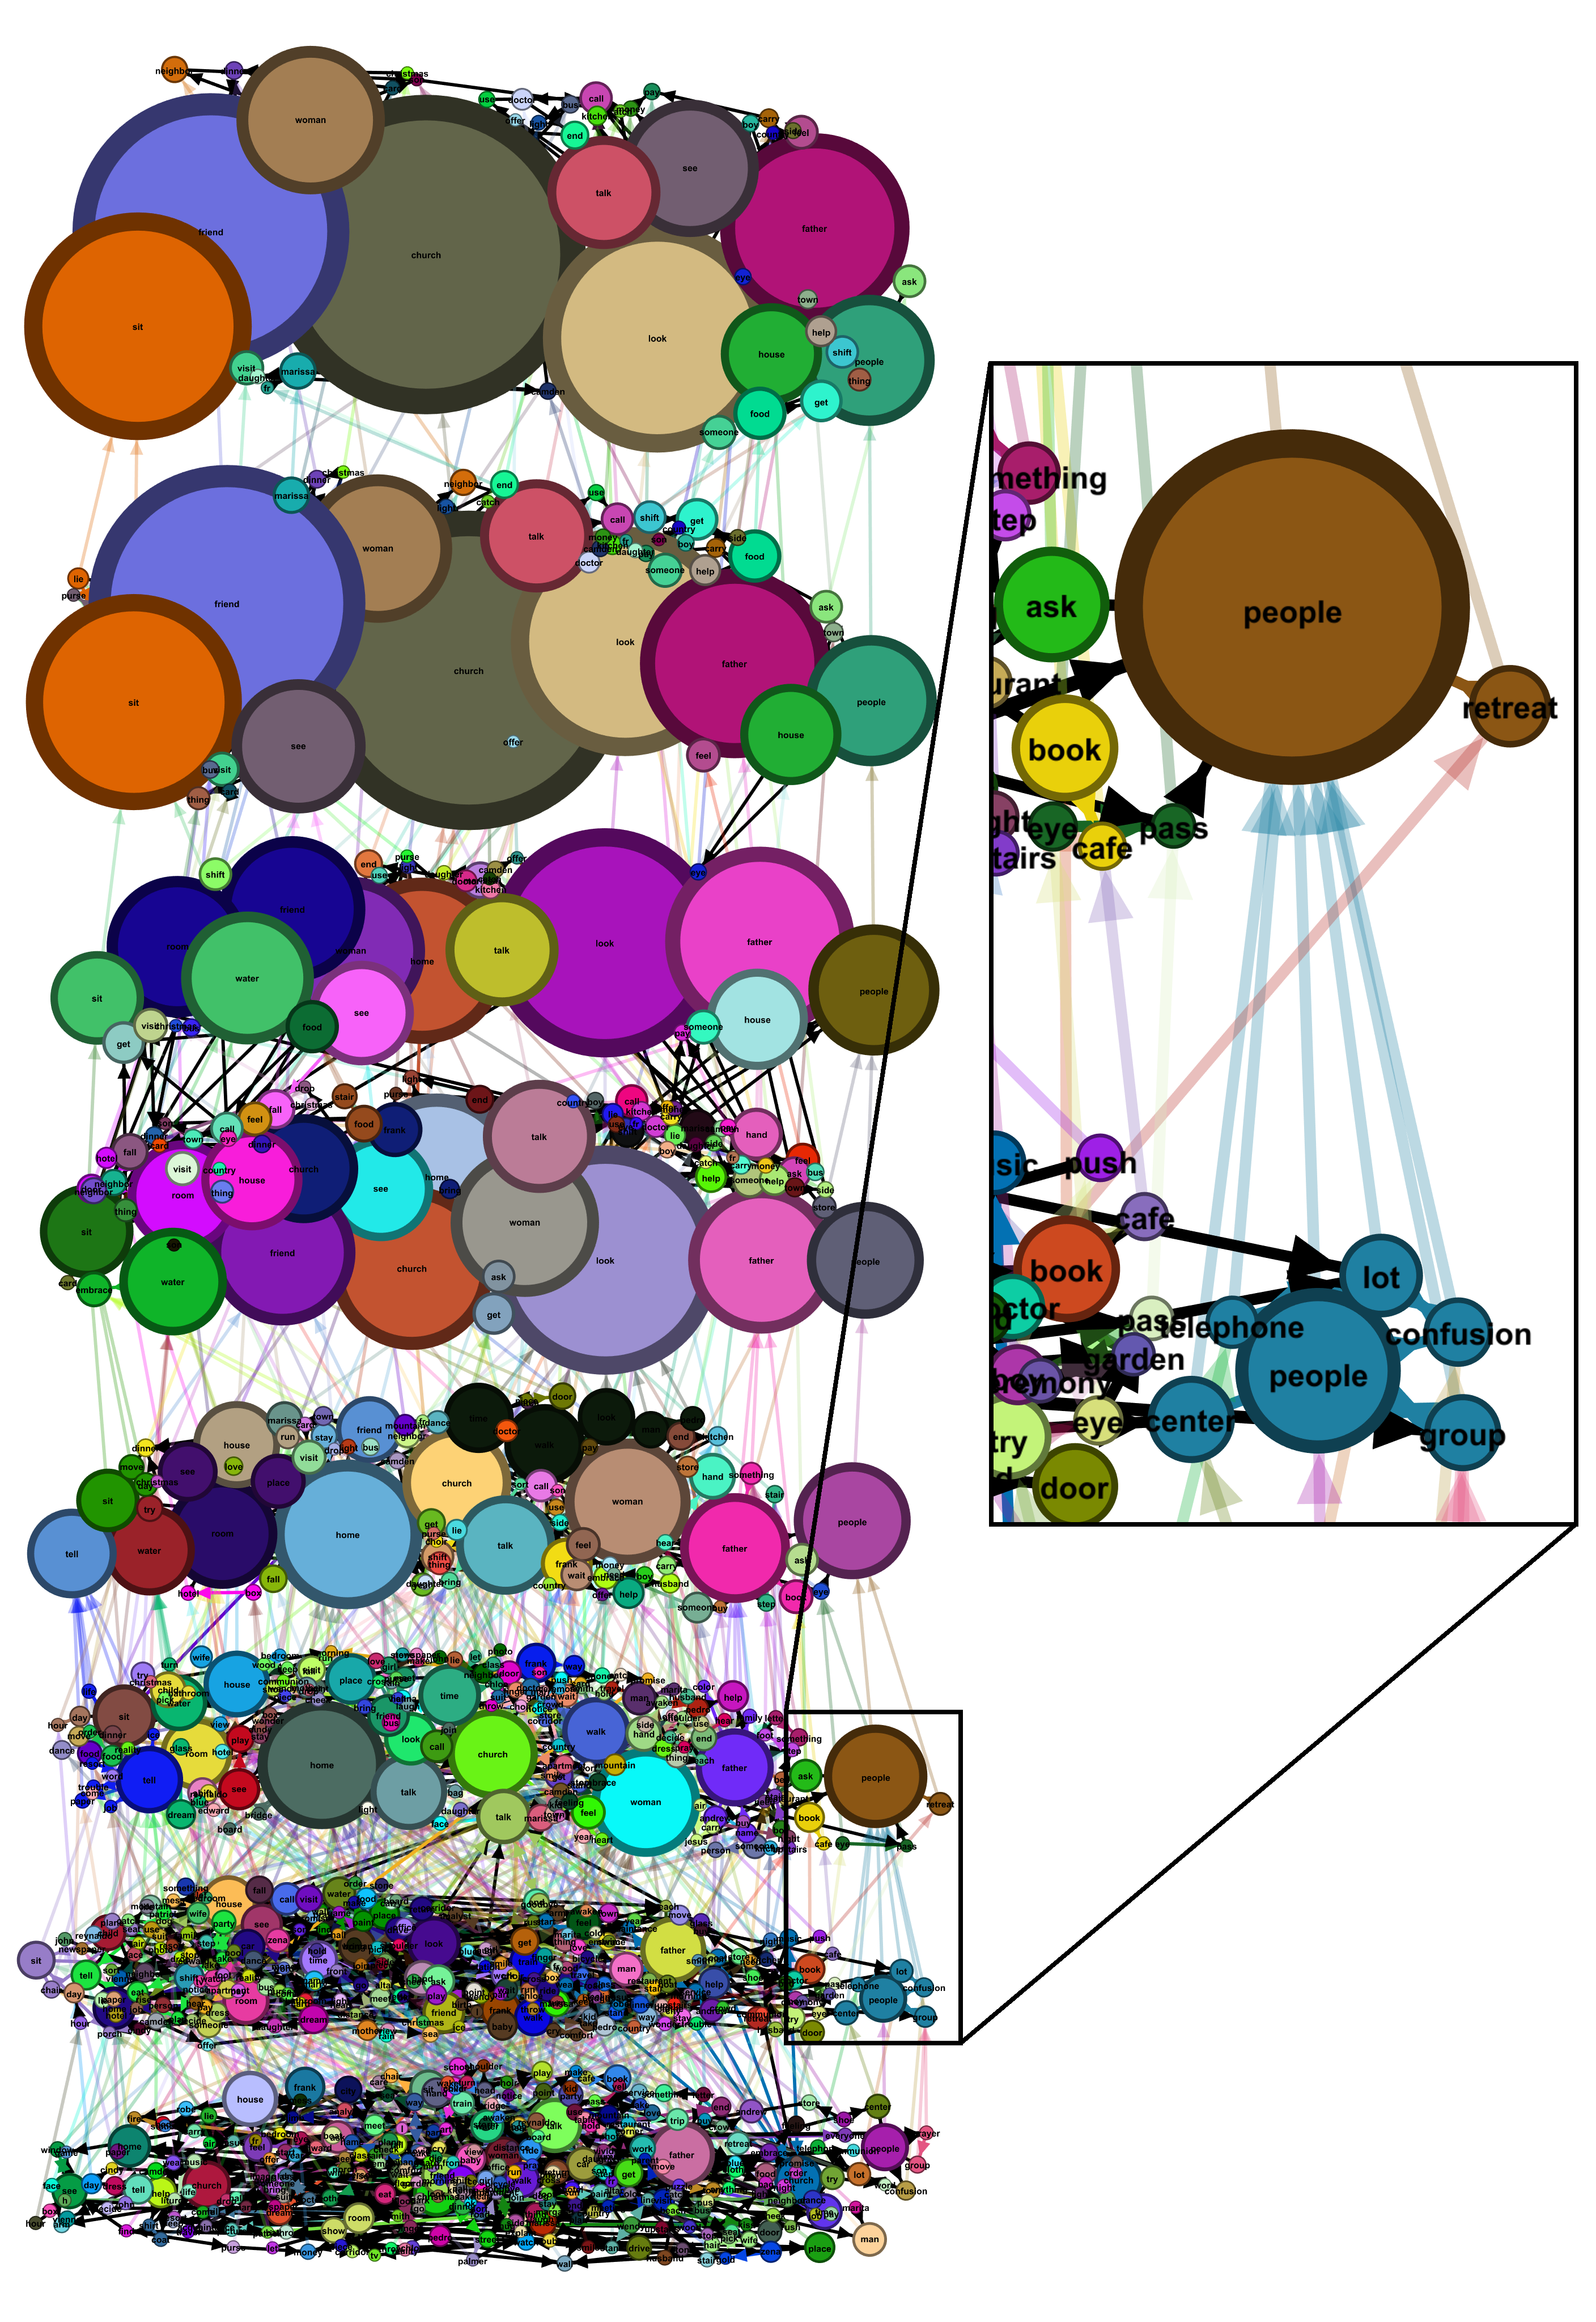
\includegraphics[width=1\textwidth]{Immagini/mlg_emma_focus_example}
    \caption{Grafo multi-livello del corpus di sogni di Emma}
    \label{fig:mlg-emma-example}
\end{figure}

Il rilevamento dei cicli, che identifica sequenze rilevanti di parole che riportano alla parola iniziale, potrebbero
rappresentare schemi influenti o temi ricorrenti nelle narrazioni dei sogni,
potenzialmente indicando collegamenti di pensiero persistenti nei sogni di Emma.
Si noti tuttavia che per l'elevato numero di sogni considerati e per la conseguente scelta del parametro di threshold,
la presenza di cicli è limitata a poche brevi sequenze di parole particolarmente correlate, date da gruppi di
parole come ``cake''-``party'', ``boat''-``lake''-``water'', ``trip''-``train''-``station'' oppure
``road''-``car''-``drive''-``hill''.
\'E interessante fare supposizioni su come queste sequenze possano fornire delle informazioni rilevanti proprio per
via del forte legame semantico che esse rappresentano.
Ad esempio la sequenza ``liturgy''-``church'-``music'' potrebbe indicare che per Emma il tema della musica è
fortemente associato al contesto della chiesa e alla liturgia, rispetto ad altri contesti che potrebbero
essere maggiormente attinenti per altre persone, come quello di un concerto o di un'accademia musicale.


L'individuazione delle componenti fortemente connesse al livello successivo potrebbe indicare unità tematiche coerenti
che, nel complesso delle narrazioni dei sogni, si co-occorrono e si interconnettono frequentemente tra loro rendendosi
mutualmente raggiungibili.
Queste componenti potrebbero rappresentare cluster di concetti o temi strettamente
interrelati che frequentemente co-occorrono e si interconnettono tra più sogni.
Come si può dedurre confrontando le dimensioni dei nodi al livello $2$ rispetto a quelle del livello precedente,
l'applicazione della contrazione per componenti fortemente connesse, in genere permette di individuare contesti
semanticamente più ampi di quelli visti per la contrazione per circuiti semplici.
Questo è dovuto da un lato alla natura delle componenti stesse, da un altro al fatto che la contrazione avviene
già ad un livello di astrazione superiore, in cui concetti strettamente collegati sono già stati raggruppati in unici
supernodi.
Esempi di insiemi di lemmi originali contenuti in componenti fortemente connesse individuate sono
``sit''-``chair''-``front''-``porch''-``seat''-``plane''
oppure ``lake''-``boat''-``water''-``rise''-``pool''-``swim''-``rush'', che racchiude uno dei circuiti semplici visti
in precedenza.

La contrazione per stelle, infine, permette di inglobare ulteriormente dei supernodi periferici ai quelli principali già
affermati nei primi livelli.
In questo modo lemmi e contesti che ``orbitano'' attorno ad altri e che, quindi,
ne siano strettamente dipendenti, vengono contratti in contesti più generali, espandendosi di una singola unità
di distanza di un arco ad ogni successivo livello.
Lo scopo di queste contrazioni altro non è che quello di far nascere dei macro-cluster che includano la maggior parte
delle parole originali, in maniera simile a come accade per alcuni strumenti di NLP, come i modelli di
\textit{word embedding}, le tecniche di \textit{topic modeling} e algoritmi di clustering semantico.
\section{Analisi delle differenze sintattiche tra sognatori} \label{sec:analisi-delle-differenze-sintattiche-tra-sognatori}

Come anticipato nel Capitolo~\ref{cap:mondo-dei-sogni}, nel contesto psichiatrico la rappresentazione di testi sui
sogni attraverso grafi si \`e rivelato un utile strumento a supporto della diagnosi di disturbi come la schizofrenia
o il disturbo bipolare~\cite{mota2014graph}, nonch\'e la possibilit\'a di predire l'insorgenza di patologie in
anticipo rispetto alla diagnosi clinica~\cite{mota2017thought}.
Tali studi evidenziando di come l'attenzione ad aspetti sintattici della descrizione di sogni possano fornire
informazioni significative sullo stato mentale di un individuo. Costruendo grafi in cui i nodi corrispondono a parole
e gli archi ad un loro utilizzo consecutivo, si è rivelato utile valutare aspetti come la presenza di cicli di parole
ricorrenti, la connettivit\'a delle parole e la loro organizzazione in componenti fortemente connesse.

In questa sezione verrà illustrata una possibile metodologia di analisi sintattica dei testi di singoli sogni mediante
grafi multi-livello, applicandola ai sogni di un campione di tre sognatori: Arlie, Emma e Norman.
In particolare, si cercherà di potenziare la modalità di studio proposta dalle ricerche citate, tentando di estenderla
grazie alla visione globale fornita dal grafo multi-livello e alla focalizzazione sugli aspetti che caratterizzano
l'evoluzione dei grafi delle parole nel corso delle contrazioni.

\subsection{Fase di pre-elaborazione}\label{subec:pre-elaborazione-con-NLP}
Prima di applicare la vera e propria analisi attraverso l'impiego dei grafi multi-livello al dataset di sogni, si è
ritenuto necessario effettuare una pre-elaborazione dei testi attraverso gli strumenti tipici dell'elaborazione del
linguaggio naturale.
L'NLP (in inglese \textit{Natural Language Processing}) è di fatti quella disciplina a metà tra intelligenza artificiale
e linguistica che si occupa di individuare i metodi di elaborazione e analisi di dati che si presentano sotto forma di
linguaggio naturale, ovvero di linguaggi usati dell'essere umano. \newline

La pre-elaborazione ha quindi previsto l'applicazione della seguente sequenza di fasi al corpus di sogni originario:
\begin{enumerate}
    \item \textbf{Pulizia del testo} \newline \noindent
          Questa fase ha incluso la rimozione degli spazi bianchi superflui, la standardizzazione della
          formattazione del testo e la correzione di errori ortografici o di incoerenze. È stata inoltre eseguita la
          rimozione della punteggiatura, snellendo ulteriormente i dati testuali. Tali procedure di pulizia sono
          essenziali per garantire la qualità e la coerenza dei dati in ingresso, migliorando così l'affidabilità
          dell'analisi.
    \item \textbf{Tokenizzazione} \newline \noindent
          Questa fase ha comportato la suddivisione del testo in parole singole dette \textit{token},
          passaggio fondamentale nell'elaborazione del linguaggio naturale, creando la base per le fasi successive.
    \item \textbf{Rimozione delle stop words} \newline \noindent
          Le \textit{stop words} sono parole comuni (come ``the'', ``is'', ``at'', ``which'' e ``on'') che tipicamente
          non hanno un ruolo significativo nei compiti di NLP, specialmente in quelli legati ad analisi semantiche.
          In questo caso, la loro rimozione può certamente aiutare a concentrare l'analisi sulle parole più ricche di
          contenuto nelle narrazioni dei sogni, riducendo significativamente il rumore nei dati e mettendo in evidenza
          i termini più salienti.
    \item \textbf{Lemmatizzazione} \newline \noindent
          La lemmatizzazione è un processo che riduce le parole alla loro forma base, chiamata \textit{lemma}.
          Ad esempio, ``running'' verrebbe lemmatizzato in ``run'' e ``better'' in ``good''.
          Questo passaggio aiuta a ridurre le diverse declinazioni delle parole ai loro concetti di base, riducendo
          la dimensionalità dei dati testuali e rivelando, potenzialmente, schemi sottostanti in modo più chiaro.
    \item \textbf{Costruzione del grafo delle parole} \newline \noindent
          Infine, è stato costruito un grafo diretto basato sulle singole parole all'interno delle sequenze
          di lemmi associate a ogni sogno. Tali parole, in quanto prese singolarmente rispetto alla sequenza
          di appartenenza, si definiscono \textit{unigrammi}. In questo grafo, quindi, ogni nodo rappresenta
          un unigramma univoco, con una proprietà ``peso'' che indica il numero di occorrenze di quell'unigramma
          nell'intero corpus di sogni.
          Gli archi orientati del grafo collegano gli unigrammi dei lemmi che appaiono seguitamente nella
          sequenza associata ad ogni sogno.
          Per questo motivo, ad ogni arco corrisponde un \textit{bigramma}, ovvero un accostamento ordinato di due parole.
          Il peso di ciascun arco rappresenta il numero di occorrenze di quello specifico accostamento ordinato nel testo.
          In questo modo, la struttura del grafo cattura non solo le relazioni sequenziali tra le parole nei sogni,
          ma anche la frequenza e la forza di queste parole e relazioni.
\end{enumerate}

\begin{figure}[h!]
    \centering
    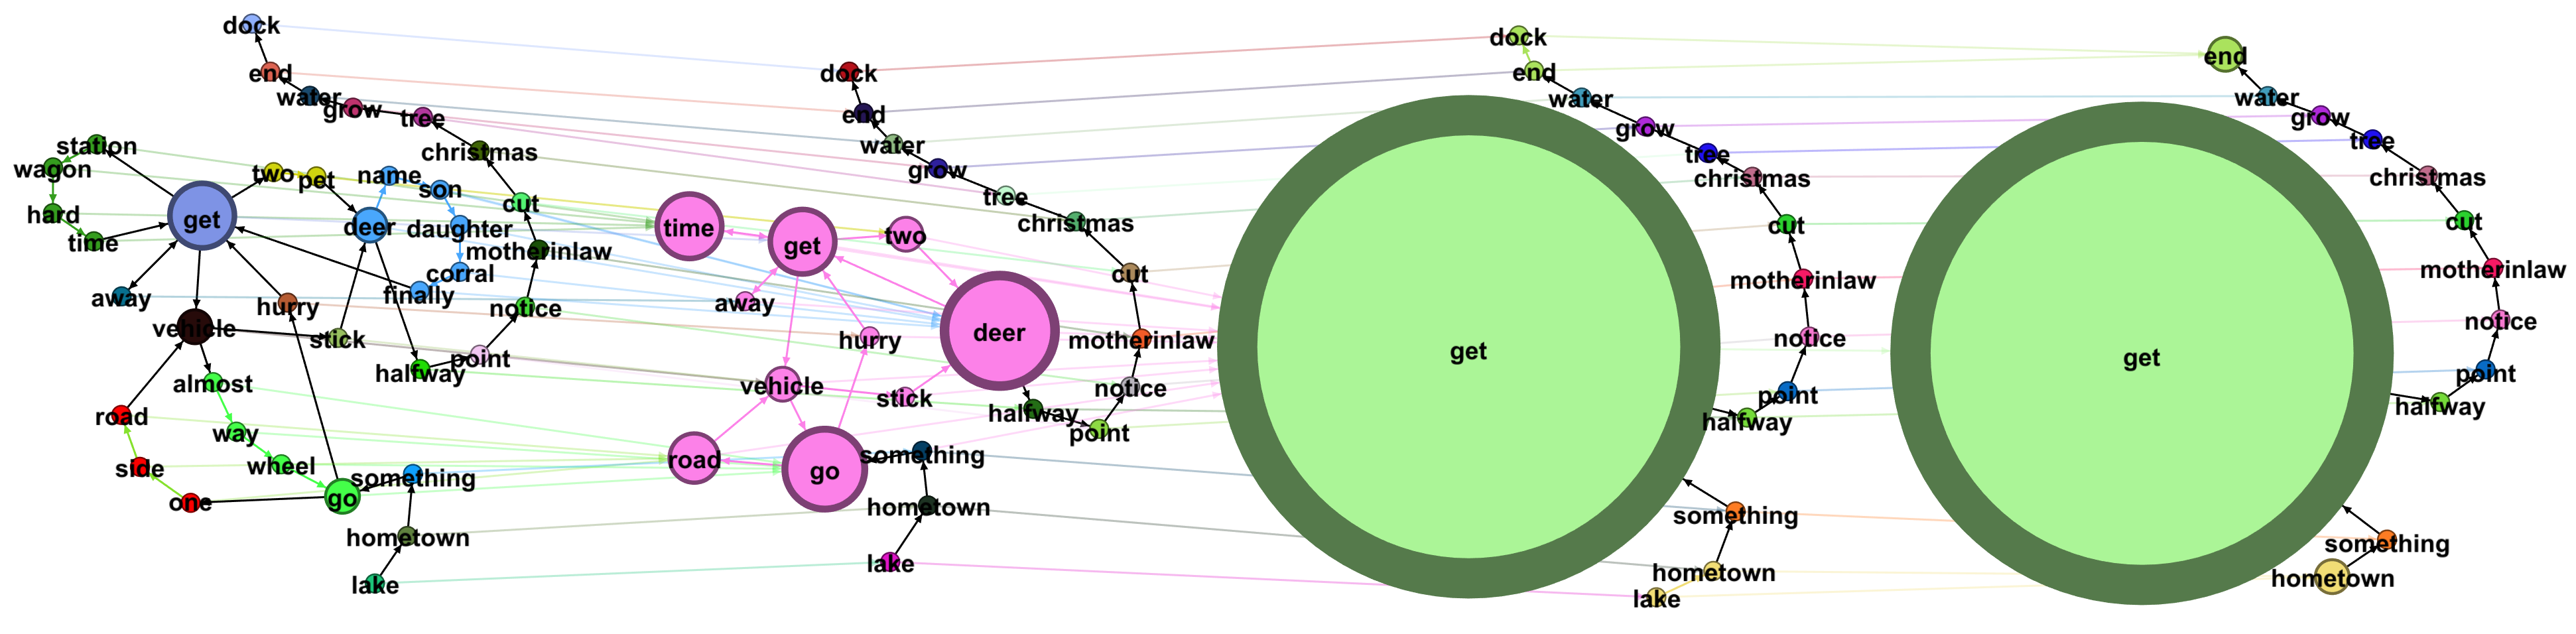
\includegraphics[width=1\textwidth]{Immagini/arlie_dream_graph_example}
    \caption{Grafo multi-livello di un sogno di Arlie}
    \label{fig:arlie-dream-graph}
\end{figure}

Utilizzando il grafo delle parole $G$ così prodotto come input per la costruzione di grafo multi-livello
$M = (G, \Gamma)$, è quindi stato possibile rappresentare i sogni di Emma, Arlie e Norman in un'unica struttura,
dove i supernodi rappresentano parole, concetti e pensieri a diversi livelli di astrazione, mentre i super-archi
rappresentano le relazioni tra tali elementi quando sono correlati.
In Figura~\ref{fig:arlie-dream-graph} è mostrato un esempio di grafo delle parole costruito a partire da un sogno di Arlie, e dei
relativi livelli di astrazione ottenuti attraverso la contrazione del grafo.
In particolare, l'esempio mostra il grafo multi-livello risultante dall'applicazione di schemi di contrazione per
circuiti semplici, componenti fortemente connesse e stelle.
La funzione di contrazione per stelle rappresenta un ulteriore livello di astrazione in cui tutti i nodi su cui è
incidente un unico arco che li collega ad un nodo centrale vengono contratti in un unico supernodo.
Nel caso delle parole, il centro di una stella può rappresentante il concetto di base comune a tutti i nodi contratti,
in quanto loro unico punto di collegamento con le altre parole del grafo.

I grafi multi-livello così prodotti sono stati quindi utilizzati come base per l'analisi multi-livello dei sogni,
come descritto nella sezione successiva.

\subsection{Analisi dei risultati}
A partire dall'analisi di un dataset di narrazioni di sogni provenienti da sedici individui si è seguita la
metodologia precedentemente descritta, raccogliendo dati statistici sulle caratteristiche topologiche
dei grafi a vari livelli delle gerarchie prodotte per ciascun sognatore.
In questa parte l'attenzione verrà rivolta a tre particolari sognatori dei sedici originali: Arlie, Emma e Norman.
Arlie è stata identificata come un sognatrice con grafi delle parole aventi parametri strutturali che più si
avvicinano alle medie del campione, mentre Emma e Norman sono stati scelti per alcune caratteristiche atipiche
che li differenziano dal resto del gruppo.

Il grafo multi-livello $M = (G, \Gamma)$ scelto per l'elaborazione del grafo delle parole $G$ prodotto a partire
da ciascun sogno prevede una sequenza di sette funzioni di contrazione che sono, rispettivamente:
\begin{itemize}
    \item \eqmakebox[things][l]{$f_{C_1}$}
    $ \begin{aligned}[t]
      \text{funzione di contrazione per circuiti semplici.}
      \end{aligned} $
    \item \eqmakebox[things][l]{$f_{C_2}$}
    $ \begin{aligned}[t]
      \text{funzione di contrazione per componenti fortemente connesse.}
      \end{aligned} $
    \item \eqmakebox[things][l]{$f_{C_3},\ldots,f_{C_7}$}
    $ \begin{aligned}[t]
      \text{funzioni di contrazione per stelle.}
      \end{aligned} $
\end{itemize}

Ciascuno dei grafici presentati a seguire comprende tre traiettorie distinte, ognuna corrispondente ai dati
dei tre sognatori selezionati, ottenuti da un insieme di 221, 1252 e 669 narrazioni, rispettivamente.
Per ciascun insieme di narrazioni legate ai particolari sognatori, si sono selezionati i sogni con un numero di
occorrenze di lemmi compreso tra 15 e 300 per narrazione, approssimativamente corrispondenti a sogni
di lunghezze che variano dalle 30 alle 750 parole.
I grafici mostrano l'evoluzione di una certa proprietà dei grafi a ciascun livello della gerarchia,
dove il livello $0$ rappresenta la struttura originale del grafo.
L'asse delle ordinate quantifica la proprietà, mentre l'asse delle ascisse delinea i livelli del grafo multi-livello.

A causa della significativa variazione nel numero medio di lemmi tra le narrazioni dei sognatori — per precisione
48,47 per Arlie, 38,57 per Emma e 28,80 per Norman — i dati sensibili alla lunghezza del sogno sono stati normalizzati a un
valore percentuale relativo al conteggio dei lemmi del sogno originale.
A partire da osservazioni effettuate sul dataset, infatti, dati come il numero di nodi e archi, il peso dei nodi,
la dimensione degli insiemi componente e il numero (ma non la lunghezza) delle basi cicliche risultano essere tutti
linearmente influenzati dal numero di lemmi considerati in ciascun sogno.

\newpage

\begin{wrapfigure}{R}{0.5\textwidth}
    \vspace{-5pt}
    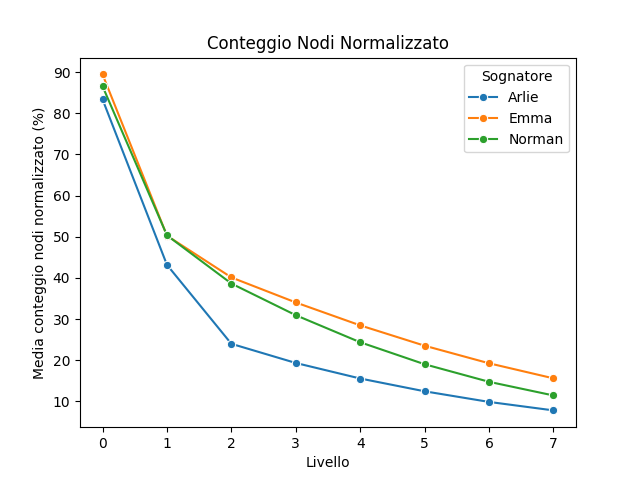
\includegraphics[width=0.55\textwidth]{Immagini/conteggio_nodi_normalizzato}
    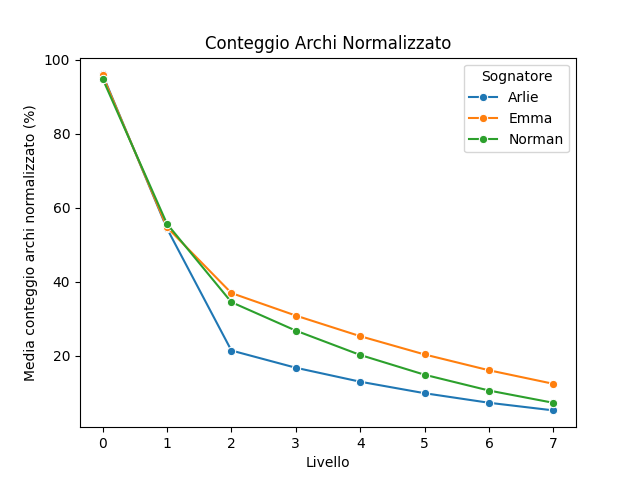
\includegraphics[width=0.55\textwidth]{Immagini/conteggio_archi_normalizzato}
    \caption{Statistiche sulle dimensioni dei grafi}\label{fig:node_edge_count}
    \vspace{-5pt}
\end{wrapfigure}

Nella Figura~\ref{fig:node_edge_count}, in alto, è mostrato il grafico del conteggio dei nodi, il quale illustra
l'evoluzione della quantità di nodi nei vari livelli.
I cali significativi delle traiettorie che scendono velocemente a partire da un valore alto indicano una struttura
di nodi inizialmente complessa che subisce una rapida semplificazione.
I dati di Arlie mostrano una discesa più ripida, suggerendo una veloce contrazione della struttura iniziale sin
dai primi schemi di contrazione.
I dati di Norman ed Emma presentano un tasso di declino più contenuto, mantenendo una riduzione coerente rispetto
allo specifico schema di contrazione, indicativo di strutture meno organizzate.

Il grafico del conteggio degli archi imita l'analisi ottenuta dal conteggio dei nodi, fornendo un'idea più chiara
della complessità delle strutture.
Analogamente al conteggio dei nodi, un valore iniziale alto sulle ordinate seguito da un brusco calo suggerisce
una connettività iniziale densa che subisce una significativa semplificazione.
I dati sui sogni di Arlie mostrano una densità di archi ordinaria con un marcato declino al livello $2$, indicando una
sostanziale interconnessione di parole.
Essendo che tali interconnessioni derivano da una quantità di archi al livello $1$ proporzionalmente
paragonabile a quella degli altri due sognatori, questo aspetto potrebbe suggerire una maggiore qualità delle relazioni
tra le parole nei sogni di Arlie, intesa come una più equa distribuzione degli archi tra parole e cicli di parole.

\begin{wrapfigure}{L}{0.5\textwidth}
   \vspace{-5pt}
    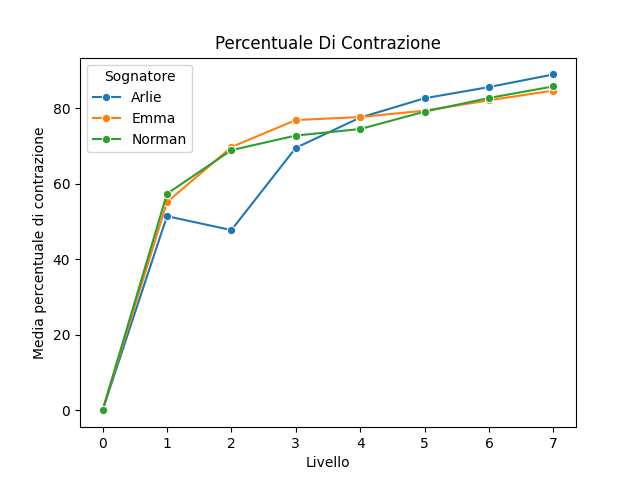
\includegraphics[width=0.55\textwidth]{Immagini/percentuale_di_contrazione}
    \caption{Statistiche sulla contrazione}\label{fig:contraction_percentage}
   \vspace{-5pt}
\end{wrapfigure}

Il grafico in Figura~\ref{fig:contraction_percentage} permette di arricchire la visione fornita dai grafici precedenti,
mostrando la percentuale di contrazione dei nodi di ciascun livello, calcolata considerando la quantità di nodi del
livello rispetto a quella del livello precedente.
Le linee indicano che, mentre Emma e Norman presentano solo lievi differenze nelle prime contrazioni per stelle, i dati
di Arlie mostrano una divergenza più significativa nel processo di contrazione delle componenti fortemente connesse.
Questa informazione, combinata con le quelle fornite dai grafici precedenti, suggerisce che molti nodi vengono esclusi
dalle aggregazioni principali, portando a una struttura più frammentata.
Tuttavia, questa struttura si semplifica rapidamente nei livelli successivi, indicando che la maggior parte dei nodi
orbita nelle immediate vicinanze di massicce aggregazioni principali.

\begin{wrapfigure}{R}{0.5\textwidth}
    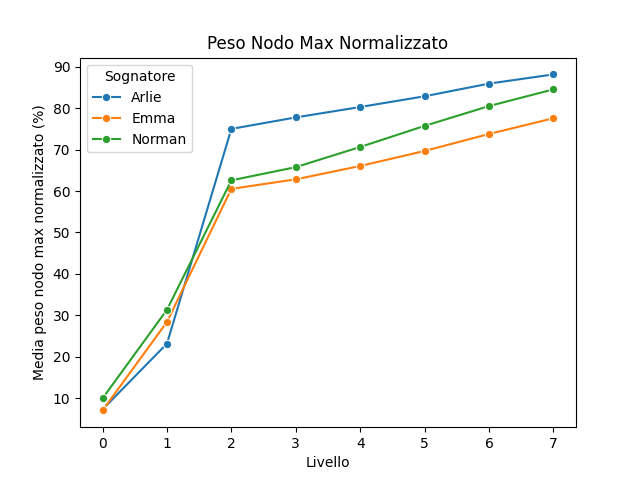
\includegraphics[width=0.55\textwidth]{Immagini/peso_nodo_max_normalizzato}
    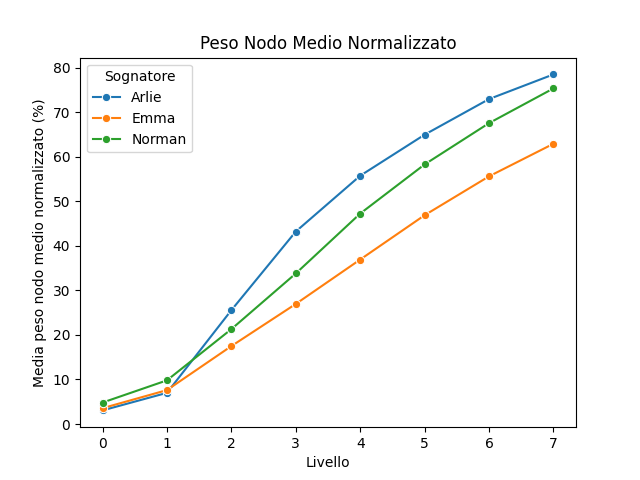
\includegraphics[width=0.55\textwidth]{Immagini/peso_nodo_medio_normalizzato}
    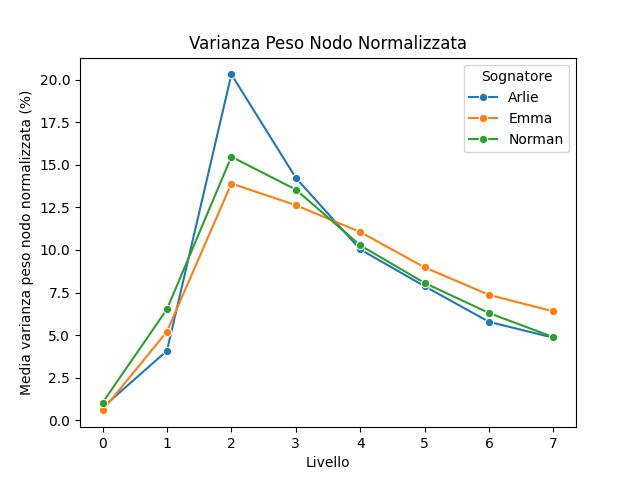
\includegraphics[width=0.55\textwidth]{Immagini/varianza_peso_nodo_normalizzata}
    \caption{Statistiche sui pesi dei nodi}\label{fig:node_weight}
\end{wrapfigure}

In Figura~\ref{fig:node_weight} i grafici danno un'idea dell'evoluzione della distribuzione del peso dei nodi.
Al livello iniziale, i dati di Arlie mostrano un peso medio dei nodi moderato, seguito da un marcato aumento nel
corso dei livelli superiori.
Questo modello suggerisce che, mentre le strutture iniziali possiedono nodi di moderata importanza,
l'aggregazione per componenti fortemente connesse amplifica particolarmente la loro rilevanza, risultando in
aggregazioni altamente pesanti.
Ciò non risulta particolarmente evidente nel caso degli altri due sognatori che mantengono un incremento del peso
medio più tendente al rettilineo.
In particolare, i dati di Emma dimostrano un aumento moderato ma costante del peso medio dei nodi, indicativo di
una struttura iniziale equilibrata in cui i nodi acquisiscono gradualmente importanza attraverso i livelli successivi.
D'altra parte, i dati di Norman mostrano un aumento leggermente più pronunciato, a partire dai cicli fino ai
livelli superiori, riflettendo una più bassa dispersione delle singole parole rispetto a Emma, e una maggiore
inclinazione all'aggregazione, specialmente per le formazioni a stella.
Il grafico della varianza sul peso dei nodi fornisce informazioni sull'equilibrio interno delle strutture rispetto
alla loro importanza.
I dati di Arlie mostrano un forte aumento della varianza, con un picco notevole al livello $2$, indicando una convergenza
di molti nodi verso poche aggregazioni altamente significative ed evidenziando nuovamente l'importanza delle componenti
fortemente connesse nel processo di aggregazione.
I dati di Emma presentano una varianza più alta ai livelli superiori, suggerendo la frequente presenza di nodi
poco pesanti che rimangono distaccati dalle aggregazioni principali e che, quindi, sono generalmente distanti, poco
connessi o situati in fondo a cammini che rappresentano vicoli ciechi.

\newpage

\begin{wrapfigure}{L}{0.5\textwidth}
    \vspace{-10pt}
    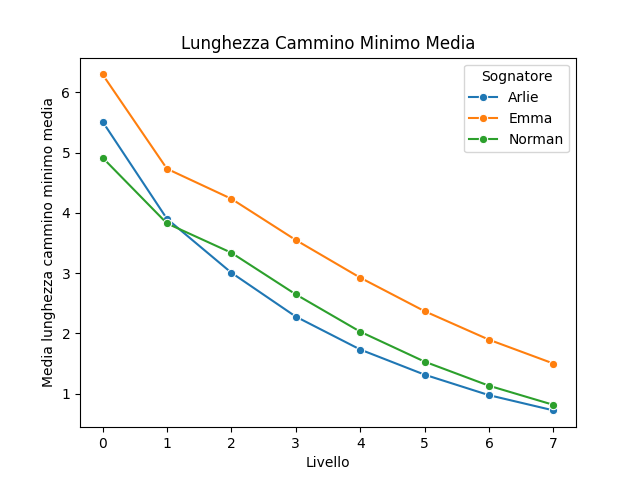
\includegraphics[width=0.55\textwidth]{Immagini/lunghezza_cammino_minimo_media}
    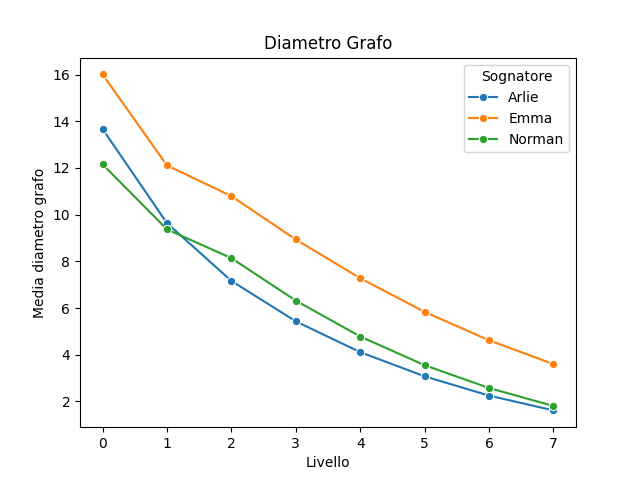
\includegraphics[width=0.55\textwidth]{Immagini/diametro_grafo}
    \caption{Statistiche sui cammini}\label{fig:paths}
    \vspace{-10pt}
\end{wrapfigure}

Il grafico delle medie dei cammini minimi in Figura~\ref{fig:paths} rappresenta l'evoluzione della lunghezza media di
tali cammini attraverso i diversi livelli dei grafi.
La misura è calcolata sulla versione non orientata di ciascun grafo come la distanza media tra ciascuna coppia di
nodi in termini di archi.
Valori iniziali più alti indicano strutture iniziali più estese, le quali normalmente riducono tale caratteristica
contraendosi attraverso i livelli successivi.
I dati di Emma iniziano con cammini mediamente lunghi, da cui si deduce la presenza percorsi inizialmente isolati
che diventano via via più compatti rispetto al resto del grafo, specialmente con la contrazione dei cicli.
Tuttavia, i grafi delle parole di Emma dimostrano di mantenere un'elevata lunghezza media, corroborando l'ipotesi
della frequente presenza di lunghi vicoli ciechi.
I dati di Norman mostrano cammini di lunghezze più moderate, imitando l'andamento di Emma,
mentre i dati di Arlie presentano cammini inizialmente più lunghi e con declino più graduale, indicando strutture di
percorso più semplici.
Il secondo grafico nella stessa figura mostra l'evoluzione del diametro del grafo, parametro strettamente legato
alla lunghezza dei cammini minimi, definito come il cammino minimo di lunghezza massima tra tutte le coppie di nodi.
Diametri iniziali più alti indicano strutture più estese.
Questo grafico segue accuratamente quello precedente, indicando che, per tutti e tre i sognatori, le forme del grafo
tra i livelli non sono deformate e contengono nodi approssimativamente equidistanti.

Il grafico del conteggio delle basi cicliche in Figura~\ref{fig:cycle_basis} quantifica la presenza di collegamenti
circolari tra parole o gruppi di parole, considerando la versione non orientata dei grafi.
Le basi cicliche rappresentano i cicli fondamentali del grafo non ulteriormente scomponibili in sotto-cicli.
Sono dette ``basi'' in quanto a partire da esse è possibile comporre tutti gli altri cicli attraverso una operazione di
unione degli archi che li compongono in or esclusivo.
I dati di Norman mostrano un alto conteggio iniziale dei cicli seguiti da un brusco calo, indicando la presenza di molti
cicli orientati tra le basi cicliche che vengono riconosciute nella prima funzione di contrazione.
I dati di Arlie presentano più basi cicliche che non sono facilmente contratte al primo livello di contrazione,
indicando una maggiore presenza di connessioni cicliche nascoste che non seguono un semplice percorso unidirezionale.
I dati di Emma mostrano meno cicli con una diminuzione costante, indicando la presenza di strutture più lineari.
Queste informazioni, combinate ai dati del grafico sulla lunghezza delle basi cicliche, suggeriscono che i sogni di
Norman contengono più cicli, anche se più piccoli, mentre i sogni di Emma contengono una minor quantità di cicli,
seppur generalmente più grandi.
Tuttavia, la distinzione sulla lunghezza tra Emma e Arlie può essere osservata solo nel grafo al livello $1$, suggerendo
che, a differenza di Arlie, le basi cicliche di Emma sono ottenute prevalentemente da insiemi di parole che si
conseguono nella narrazione originale del sogno, nonostante consistano di un alto numero di lemmi.

\begin{figure}[t]
    \hspace{-5pt}
    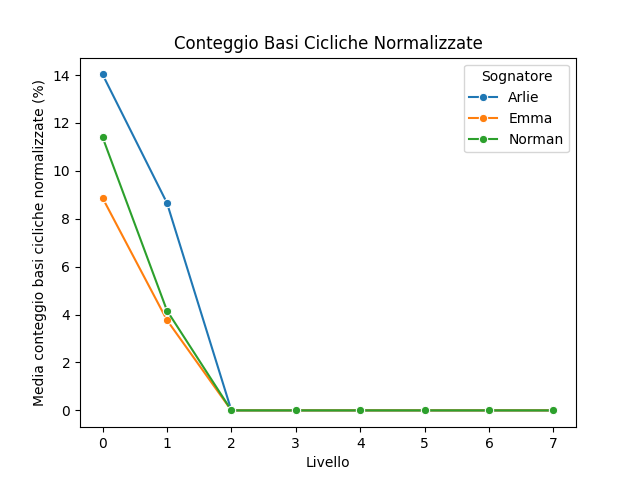
\includegraphics[width=0.55\textwidth]{Immagini/conteggio_basi_cicliche_normalizzate}
    \hspace{-20pt}
    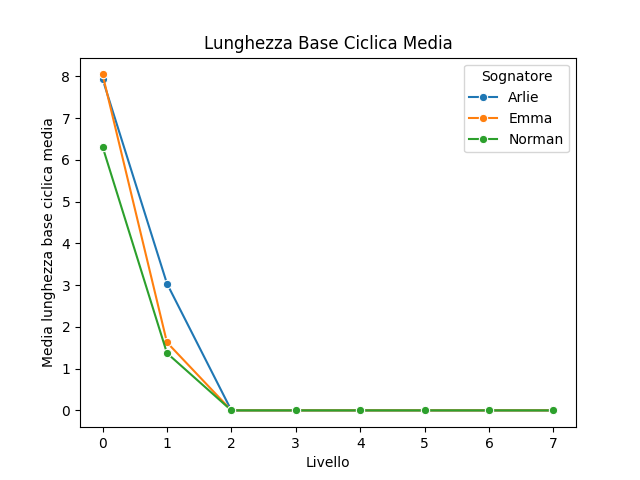
\includegraphics[width=0.55\textwidth]{Immagini/lunghezza_base_ciclica_media}
    \hspace{-5pt}
    \vspace{-10pt}
    \caption{Statistiche sulle basi cicliche}\label{fig:cycle_basis}
\end{figure}

\begin{wrapfigure}{R}{0.5\textwidth}
    \includegraphics[width=0.55\textwidth]{Immagini/densità_grafo}
    \caption{Statistiche sulla densità}\label{fig:density}
\end{wrapfigure}

La Figura~\ref{fig:density} illustra la densità media dei grafi per ciascun livello, dove la densità di un grafo è
definita come il rapporto tra il numero di archi nel grafo e il numero di archi possibili.
Tutti e tre i sognatori iniziano con basse densità iniziali del grafo che aumentano attraverso i primi livelli di
contrazione.
Oltre che essere una naturale conseguenza della riduzione della dimensione del grafo, questo indica che le strutture
iniziali di singole parole sparse diventano più interconnesse quando i nodi rappresentano aggregazioni di parole
correlate.
Le narrazioni di Arlie mostrano l'aumento di densità più elevato nel corso dei primi livelli di contrazione,
suggerendo un'interconnessione più complessa tra le componenti fortemente connesse, che si semplifica
rapidamente nei livelli successivi.
Livelli di densità bassi ai livelli superiori possono anche indicare una maggiore tendenza alla presenza di
un unico grande cluster di parole.
Osservando gli altri due sognatori, è interessante notare che, mentre i sogni di Norman mostrano una densità più alta
rispetto a quelli di Emma nei livelli iniziali, i dati dei due sognatori convergono a valori simili nei livelli
superiori, indicando un livello simile di interconnessione tra le aggregazioni principali.

\begin{figure}[t]
    \hspace{-5pt}
    \includegraphics[width=0.55\textwidth]{Immagini/coefficiente_di_assortatività_peso}
    \hspace{-20pt}
    \includegraphics[width=0.55\textwidth]{Immagini/coefficiente_di_assortatività_grado}
    \hspace{-5pt}
    \vspace{-10pt}
    \caption{Statistiche sull'assortatività}\label{fig:assortativity}
\end{figure}

Il grafico del coefficiente di assortatività dei pesi in Figura~\ref{fig:assortativity} fornisce informazioni
sull'evoluzione di tale valore tra i singoli nodi.
L'assortatività è un parametro che misura la tendenza dei nodi con determinate caratteristiche numeriche a collegarsi
con nodi aventi caratteristiche simili e, in questo caso, indica la tendenza dei nodi con pesi simili a connettersi tra
loro.
Un coefficiente positivo suggerisce la presenza di una tendenza per i temi predominanti a connettersi direttamente
tra loro, mentre un coefficiente negativo indica una tendenza per i nodi pesanti a connettersi con nodi di peso esiguo.
Questo potrebbe essere particolarmente rilevante nei livelli avanzati, dove i temi principali del sogno sono già ben
definiti.
I sogni di Norman sono soggetti ad un evidente calo dell'assortatività ai livelli alti, indicando, possibilmente,
la presenza ricorrente di una contrazione principale circondata da nodi meno importanti.
I dati di Emma, invece, mostrano una tendenza più stabile, suggerendo che le aggregazioni principali sono tipicamente
interconnesse tra loro e che non possano facilmente essere ridotte a un singolo nodo che rappresenti una formazione a
stella.

\nlparagraph{Confronto con gli studi correlati}

Studi correlati già citati, che riguardano tecniche di analisi dei sogni basate su grafi, hanno osservato differenze
nelle caratteristiche topologiche dei grafi a partire da gruppi di persone pre-classificate come sognatori sani,
schizofrenici o bipolari.
In particolare, i grafi associati ai sogni di pazienti schizofrenici sono stati valutati come grafi generalmente
piccoli e poco connessi, con basso numero di cicli, un elevato diametro rapportato alla dimensione del grafo e un
basso coefficiente di clustering, il quale indica la tendenza dei nodi a formare cluster densamente connessi.
I grafi dei pazienti bipolari, sebbene abbiano dimostrato avere un numero inferiore di caratteristiche che permettono
di distinguerli rispetto al gruppo di controllo, sono prevalentemente caratterizzati da alta connettività, alta densità
e alto coefficiente di clustering, abbinato alla maggiore presenza di cicli brevi e un basso diametro.
Tuttavia la caratteristica che ha permesso di caratterizzare e riconoscere distintamente il gruppo di controllo
dagli altri due è la presenza e la dimensione delle componenti fortemente connesse: i sognatori del controllo hanno
mostrato la dimensione maggiore tra tutti, seguiti dai bipolari e, per ultimi, gli schizofrenici. \newline

Per via del fatto che i dati ottenuti in questa analisi non sono corredati da informazioni riguardanti lo stato di
salute mentale dei sognatori, i risultati sono stati confrontati con quelli degli studi precedenti al fine
di trarre delle ipotesi su una possibile classificazione dei sognatori.
I risultati dell'analisi multi-livello si correlano alle scoperte già consolidate suggerendo che Arlie potrebbe essere
collocata nel gruppo di controllo, a causa dell'alta rilevanza delle componenti fortemente connesse nel processo di
contrazione e di altri parametri riguardanti la connettività e l'alto grado dei nodi.
Questa ipotesi è supportata dal fatto che i grafici di Arlie si conformano ai valori medi dei sedici sognatori nel
dataset.
Al contrario, Emma ha presentato caratteristiche tipiche dei pazienti schizofrenici, come un diametro del grafo
elevato e un basso coefficiente di clustering, indicando nodi poco connessi.
Dai dati di Norman, nel mentre, è emersa una rilevanza dei cicli e un alto coefficiente di clustering, che potrebbero
essere considerate qualità simili ai sogni dei pazienti bipolari.
Si noti, tuttavia, che molti altri sono stati gli aspetti emersi dall'analisi multi-livello, i quali hanno fornito una
visione più completa sui sognatori rispetto a quella che si sarebbe ottenuta da un'analisi a livello singolo.



\chapter*{Conclusioni e Sviluppi Futuri}\addcontentsline{toc}{chapter}{Conclusioni e Sviluppi Futuri}

Come appare evidente dai risultati di queste tecniche di analisi basate su grafi multi-livello, la loro applicazione
potrebbe rivelare strutture celate all'interno delle narrazioni dei sogni, che siano di natura sintattica, come
l'organizzazione del testo a livelli di astrazione superiore, o semantica, come la presenza di temi e schemi di
pensiero ricorrenti o cluster di concetti correlati.
Nell'ambito dell'analisi dei sogni, gli sviluppi futuri auspicati potrebbero riguardare l'applicazione di tali
tecniche di analisi a dati categorizzati, per rivelare correlazioni tra le strutture del grafo multi-livello
e gli stati psicologici dei sognatori, oltre che la valutazione di miglioramenti alle tecniche di contrazione e
analisi che siano ad-hoc per questo specifico dominio, come potrebbe essere la considerazione del peso degli archi
nelle funzioni di contrazione.

Tuttavia, come evidenziato da questi risultati preliminari, in generale l'approccio analitico multi-livello offre
una prospettiva globale e dinamica che va oltre l'analisi a livello singolo, rivelando strutture e relazioni complesse
all'interno dei dati.
Per questo motivo, sarebbe altrettanto interessante esplorare il comportamento di questa struttura dati in altri
domini applicativi.

Infine, un ulteriore sviluppo riguarda la progettazione di un sistema di aggiornamento dinamico
della struttura dati che permetta di aggiungere o rimuovere nuovi nodi o archi alla base della struttura
gerarchica in modo da evitare di dover ricalcolare l'intera struttura ad ogni modifica.
Questa funzionalità potrebbe essere utile per un'ulteriore tipologia di analisi che riguardi la
sensitività dei livelli più astratti alle modifiche dei dati di partenza che, declinata nell'ambito dell'analisi
dei sogni, potrebbe rivelare l'influenza di singole parole o collegamenti nella struttura complessiva.



\appendix
%\input{schema_elettrico}
%\input{Appendix1}
%\input{Appendix2}

% Citazioni nel testo
%~\nocite{*} % Include tutte le voci nel .bib, anche se non citate nel testo
% Stampa la bibliografia

\printbibliography

\printindex

%\chapter*{Ringraziamenti}

Ringrazio...

\end{document}